%
% $RCSfile: paper.tex,v $
%
% Copyright (c) 2005-2006. Christian Heller. All rights reserved.
%
% Permission is granted to copy, distribute and/or modify this document
% under the terms of the GNU Free Documentation License, Version 1.1 or
% any later version published by the Free Software Foundation; with no
% Invariant Sections, with no Front-Cover Texts and with no Back-Cover
% Texts. A copy of the license is included in the section entitled
% "GNU Free Documentation License".
%
% http://www.cybop.net
% - Cybernetics Oriented Programming -
%
% http://www.resmedicinae.org
% - Information in Medicine -
%
% Version: $Revision: 1.1 $ $Date: 2006-01-03 08:21:45 $ $Author: christian $
% Authors: Christian Heller <christian.heller@tuxtax.de>
%

% The document class specifying the type of document.
% Possible tags for headings are: section, subsection, subsubsection, paragraph.
%\documentclass[forInclusion,english]{lni}
\documentclass[english]{lni}

% Use paper format and font.
%\usepackage{a4,times}

% Graphics.
\usepackage{graphicx}

% The hyphenation list.
%
% $RCSfile: hyphenation.tex,v $
%
% Copyright (c) 2001-2004. Christian Heller. All rights reserved.
%
% No copying, altering, distribution or any other actions concerning this
% document, except after explicit permission by the author!
% At some later point in time, this document is planned to be put under
% the GNU FDL license. For now, _everything_ is _restricted_ by the author.
%
% http://www.cybop.net
% - Cybernetics Oriented Programming -
%
% http://www.resmedicinae.org
% - Information in Medicine -
%
% @author Christian Heller <christian.heller@tuxtax.de>
%

\hyphenation{abs-trac-tion}
\hyphenation{abs-trac-tions}
\hyphenation{ac-tu-ally}
\hyphenation{addi-tio-nally}
\hyphenation{ana-lyst}
\hyphenation{ana-ly-sis}
\hyphenation{an-cient}
\hyphenation{ap-pli-ca-tion}
\hyphenation{arche-types}
\hyphenation{aris-to-tle}
\hyphenation{at-tri-bute}
\hyphenation{avoi-da-ble}
\hyphenation{be-ing}
\hyphenation{binary}
\hyphenation{bran-ches}
\hyphenation{ca-te-go-ri-za-tion}
\hyphenation{client}
\hyphenation{com-po-nen-ti-za-tion}
\hyphenation{com-pu-ter}
\hyphenation{con-fi-gure}
\hyphenation{con-fi-gu-ra-tion}
\hyphenation{con-nec-ted}
\hyphenation{cri-ti-cised}
\hyphenation{cy-ber-ne-tics}
\hyphenation{cyboi}
\hyphenation{cybol}
\hyphenation{cybop}
\hyphenation{de-sign}
\hyphenation{des-cribe}
\hyphenation{des-cribed}
\hyphenation{de-ve-lop-ment}
\hyphenation{dis-crete}
\hyphenation{di-vide}
\hyphenation{do-main}
\hyphenation{dy-na-mic}
\hyphenation{dy-na-mics}
\hyphenation{ela-bo-ra-ted}
\hyphenation{ele-ments}
\hyphenation{en-gi-nee-ring}
\hyphenation{eng-lish}
\hyphenation{en-vi-ron-ment}
\hyphenation{ex-pert}
\hyphenation{fi-gure}
\hyphenation{fun-da-men-tal}
\hyphenation{func-tio-na-li-ty}
\hyphenation{hard-ware}
\hyphenation{hu-man}
\hyphenation{im-ple-men-ta-tion}
\hyphenation{imp-roved}
\hyphenation{in-he-rit}
\hyphenation{in-ter-pre-ter}
\hyphenation{java}
\hyphenation{know-ledge}
\hyphenation{lan-guage}
\hyphenation{li-ving}
\hyphenation{lo-gi-cal}
\hyphenation{machine}
\hyphenation{me-cha-nism}
\hyphenation{me-thods}
\hyphenation{na-ture}
\hyphenation{net-work}
\hyphenation{neu-ral}
\hyphenation{neu-ron}
\hyphenation{nu-me-rous}
\hyphenation{object}
\hyphenation{open}
\hyphenation{operating}
\hyphenation{ori-en-ted}
\hyphenation{over-come}
\hyphenation{prin-ci-ple}
\hyphenation{prin-ting}
\hyphenation{pro-ba-bi-lis-tic}
\hyphenation{pro-gram-ming}
\hyphenation{re-cog-nize}
\hyphenation{re-cog-nized}
\hyphenation{re-pre-sen-ta-tion}
\hyphenation{re-pre-sen-ting}
\hyphenation{re-u-sa-bi-li-ty}
\hyphenation{sci-ence}
\hyphenation{server}
\hyphenation{se-pa-ra-ted}
\hyphenation{se-pa-ra-tion}
\hyphenation{si-mi-lar}
\hyphenation{soft-ware}
\hyphenation{source}
\hyphenation{spe-cia-li-za-tion}
\hyphenation{sta-tic}
\hyphenation{sta-ti-cal-ly}
\hyphenation{sto-chas-tic}
\hyphenation{stone-on-stone}
\hyphenation{struc-ture}
\hyphenation{strug-gling}
\hyphenation{su-per-flu-ous}
\hyphenation{sup-ply-ing}
\hyphenation{sys-tem}
\hyphenation{tes-ting}
\hyphenation{thin-king}
\hyphenation{un-en-li-vened}
\hyphenation{un-fa-vou-ra-ble}
\hyphenation{un-sa-tis-fy-ing}
\hyphenation{va-ry-ing}
\hyphenation{weigh-ted}


%
% This document is a scientific paper to be handed in for a conference.
%
% @version $Revision: 1.1 $ $Date: 2006-01-03 08:21:45 $ $Author: christian $
% @author Christian Heller <christian.heller@tuxtax.de>
% @author Christian Heller <christian.heller@tu-ilmenau.de>
% @see http://www.jr-x.de/publikationen/latex/tipps/index.html
%
\begin{document}
    \twocolumn
    %
% $RCSfile: title.tex,v $
%
% Copyright (c) 2001-2004. Christian Heller. All rights reserved.
%
% No copying, altering, distribution or any other actions concerning this
% document, except after explicit permission by the author!
% At some later point in time, this document is planned to be put under
% the GNU FDL license. For now, _everything_ is _restricted_ by the author.
%
% http://www.cybop.net
% - Cybernetics Oriented Programming -
%
% http://www.resmedicinae.org
% - Information in Medicine -
%
% @author Christian Heller <christian.heller@tuxtax.de>
%

\title{A new Pattern Systematics}
\author{
    Christian Heller \(<\)christian.heller@tu-ilmenau.de\(>\)\\
    Detlef Streitferdt \(<\)detlef.streitferdt@tu-ilmenau.de\(>\)\\
    Ilka Philippow \(<\)ilka.philippow@tu-ilmenau.de\(>\)
}
\institute{Technical University of Ilmenau\\
    Faculty for Computer Science and Automation\\
    Institute for Theoretical and Technical Informatics\\
    PF 100565, Max-Planck-Ring 14, 98693 Ilmenau, Germany\\
    http://www.tu-ilmenau.de, fon: +49-3677-69-1230, fax: +49-3677-69-1220 \vspace*{0.5cm}
}

    \maketitle
    %
% $RCSfile: abstract.tex,v $
%
% Copyright (c) 2001-2004. Christian Heller. All rights reserved.
%
% No copying, altering, distribution or any other actions concerning this
% document, except after explicit permission by the author!
% At some later point in time, this document is planned to be put under
% the GNU FDL license. For now, _everything_ is _restricted_ by the author.
%
% http://www.cybop.net
% - Cybernetics Oriented Programming -
%
% http://www.resmedicinae.org
% - Information in Medicine -
%
% @author Christian Heller <christian.heller@tuxtax.de>
%

\begin{center}
    \textbf{\large{Abstract}}
\end{center}
\normalsize
\textit{
This document describes how existing design patterns can be combined to merge
their advantages into one domain- independent software framework. This framework,
called Cybernetics Oriented Programming (CYBOP), is characterized by flexibility
and extensibility. Further, the concept of Ontology is used to structure the
software architecture as well as to keep it maintainable. A Component Lifecycle
ensures the proper startup and shutdown of any systems built on top of CYBOP.\\
The practical proof of these new concepts was accomplished within the diploma
thesis of Jens Bohl which consisted of designing and developing a module called
Record, of the Open Source Software (OSS) project Res Medicinae. The major task
of this module is to provide a user interface for creating medical documentation.
New structure models such as Episodes were considered and implemented. In this
context, the integration of a graphical tool for Topological Documentation was
also highly demanded. The tool allows documentation with the help of anatomical
images and the setting of markers for pathological findings.\\
\textbf{Keywords.} Design Pattern, Framework, Component Lifecycle, Ontology,
CYBOP, Res Medicinae, Episode Based Documentation, Topological Documentation
} \rm


    %
% $RCSfile: introduction.tex,v $
%
% Copyright (c) 2005-2006. Christian Heller. All rights reserved.
%
% Permission is granted to copy, distribute and/or modify this document
% under the terms of the GNU Free Documentation License, Version 1.1 or
% any later version published by the Free Software Foundation; with no
% Invariant Sections, with no Front-Cover Texts and with no Back-Cover
% Texts. A copy of the license is included in the section entitled
% "GNU Free Documentation License".
%
% http://www.cybop.net
% - Cybernetics Oriented Programming -
%
% http://www.resmedicinae.org
% - Information in Medicine -
%
% Version: $Revision: 1.1 $ $Date: 2006-01-03 08:21:45 $ $Author: christian $
% Authors: Christian Heller <christian.heller@tuxtax.de>
%

\section{Introduction}
\label{introduction_heading}

Sometimes, describing the easy things is the most difficult. And most of the
time, it seems easier to copy existing concepts than to investigate new, but
possibly more intuitive solutions. The work described in this document tried to
question traditional concepts of software design and to correct or simplify
these by applying new ideas stemming from other scientific disciplines. It thus
wants to contribute to a better knowledge modelling.

The initially observed discrepancies belong to software engineering processes
(abstraction gaps), to the physical architecture (misleading tiers) as well as
the logical architecture (modelling mistakes) of systems. They are explained
following.

%
% $RCSfile: abstraction_gaps.tex,v $
%
% Copyright (c) 2005-2006. Christian Heller. All rights reserved.
%
% Permission is granted to copy, distribute and/or modify this document
% under the terms of the GNU Free Documentation License, Version 1.1 or
% any later version published by the Free Software Foundation; with no
% Invariant Sections, with no Front-Cover Texts and with no Back-Cover
% Texts. A copy of the license is included in the section entitled
% "GNU Free Documentation License".
%
% http://www.cybop.net
% - Cybernetics Oriented Programming -
%
% http://www.resmedicinae.org
% - Information in Medicine -
%
% Version: $Revision: 1.1 $ $Date: 2006-01-03 08:21:45 $ $Author: christian $
% Authors: Christian Heller <christian.heller@tuxtax.de>
%

\subsection{Abstraction Gaps}
\label{abstraction_gaps_heading}

Software has to be developed in a creative process called
\emph{Software Engineering Process} (SEP) or \emph{-Methodology} (figure
\ref{gaps_figure}).

\begin{figure}[htb]
    \begin{center}
        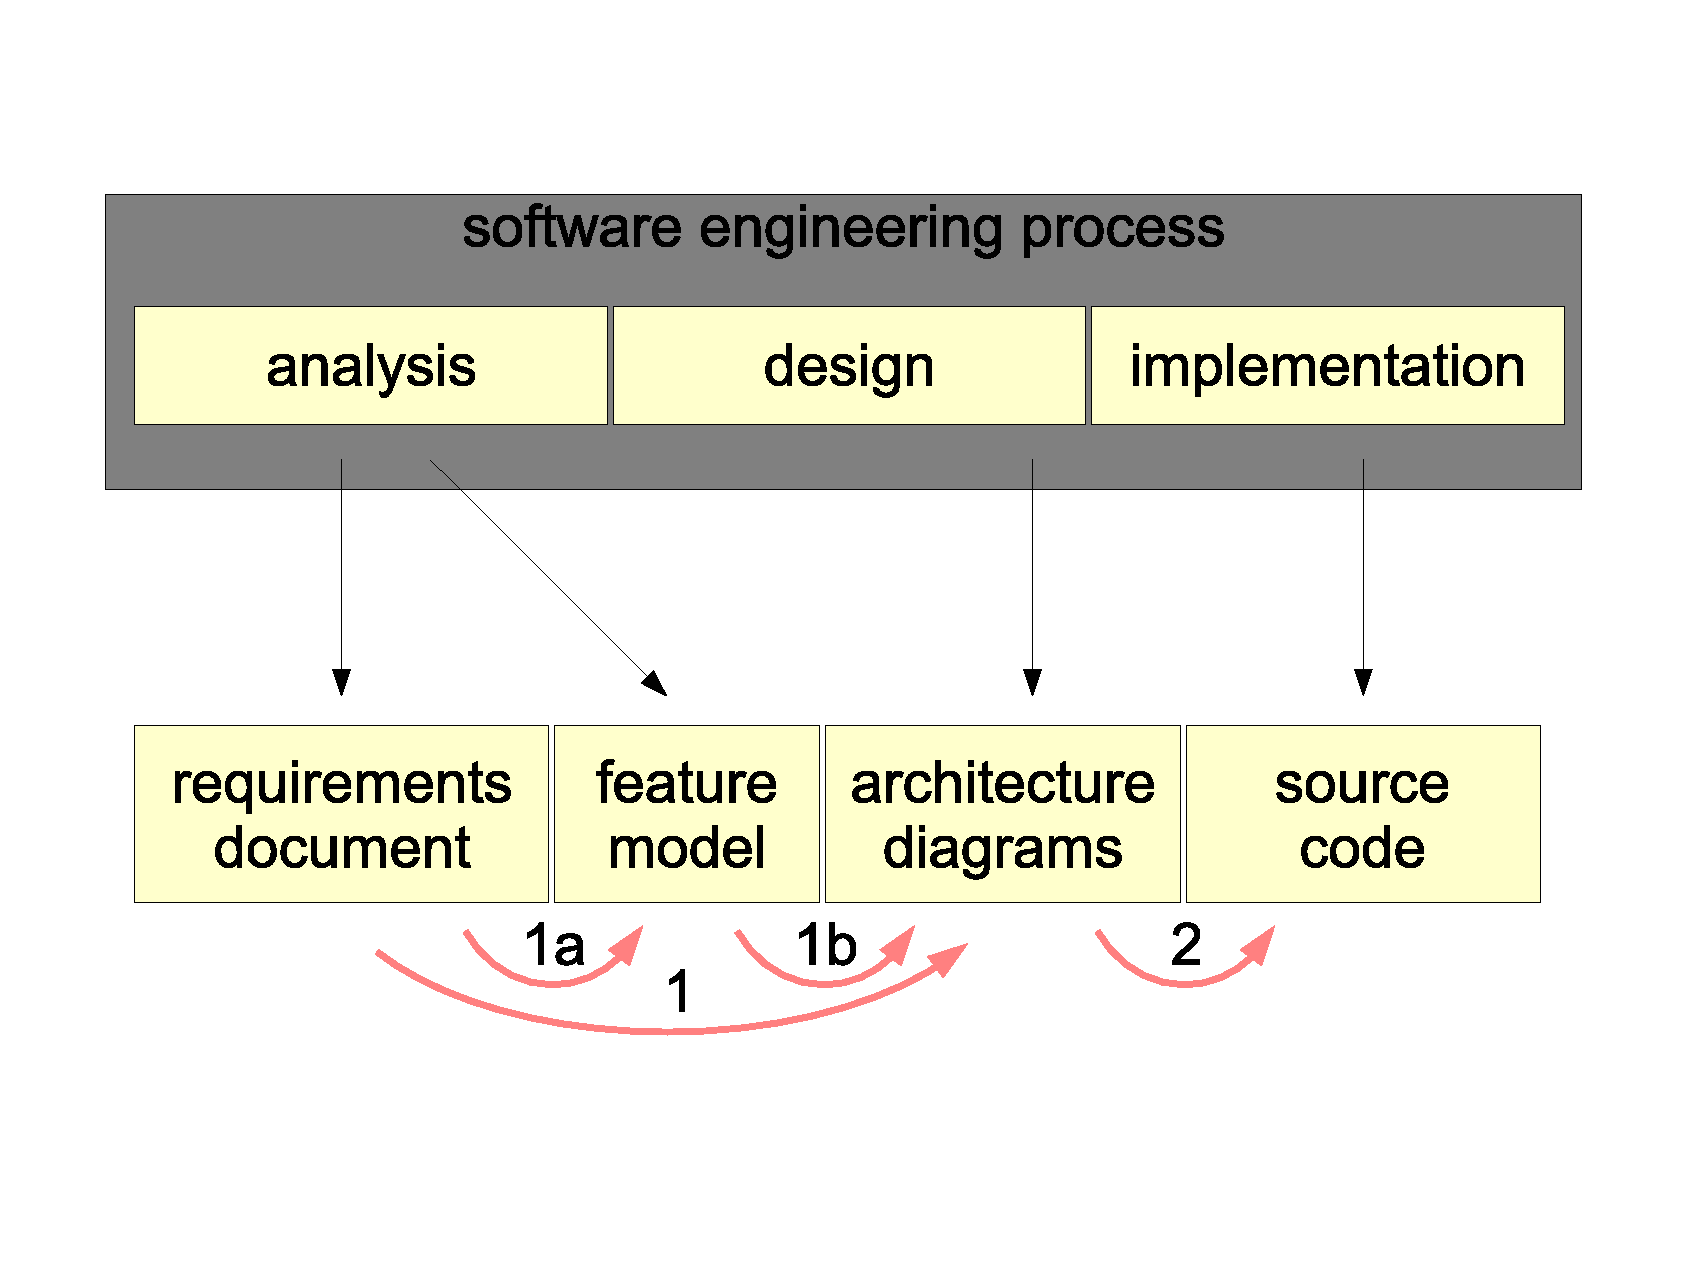
\includegraphics[scale=0.2]{vector/gaps.eps}
        \caption{Abstraction Gaps}
        \label{gaps_figure}
    \end{center}
\end{figure}

Different forms of SEP exist: \emph{Waterfall},\\ \emph{Iterative},
\emph{Extreme Programming} (XP) and \emph{Agile Programming}. But every
project, consciously or not, follows a SEP that sooner-or-later, in one form or
the other, goes through three common phases: \emph{Analysis}, \emph{Design} and
\emph{Implementation}. Each phase creates its own model of what is to be
abstracted in software and it is the differences in exactly these models that
often cause complications.

A previous article \cite{heller2004} mentioned the\\ \emph{Requirements Document},
\emph{Feature Model},\\ \emph{Architecture Diagrams} and \emph{Source Code} as
forms of knowledge abstraction. It also described the following abstraction
gaps (see figure \ref{gaps_figure}) that have to be crossed:

\begin{enumerate}
    \item[1a] Requirements Document -- Feature M.
    \item[1b] Feature Model -- Architecture Diagr.
    \item[2] Architecture Diagrams -- Source Code
\end{enumerate}

By improving the \emph{Traceability} between requirements and the architecture,
feature models (known from system family/ product line engineering) contribute
to minimising gap 1. Together with architecture diagrams, they ease
communication between stakeholders in the SEP, because of their human-readable
form and implementation-independence. But sooner-or-later, also these have to
be transferred into source code, by crossing gap 2.

Bridging or closing these abstraction gaps (sometimes called \emph{Semantic- or
Conceptual Gaps}) is also known as: \textit{achieving higher intentionality}
and remains an unsolved task for software engineering. One aim of the work
described in this article was to contribute to a possible solution, with focus
on \emph{reducing} gap 2, existing between a designed architecture and the
implemented code.

%
% $RCSfile: misleading_tiers.tex,v $
%
% Copyright (c) 2005-2006. Christian Heller. All rights reserved.
%
% Permission is granted to copy, distribute and/or modify this document
% under the terms of the GNU Free Documentation License, Version 1.1 or
% any later version published by the Free Software Foundation; with no
% Invariant Sections, with no Front-Cover Texts and with no Back-Cover
% Texts. A copy of the license is included in the section entitled
% "GNU Free Documentation License".
%
% http://www.cybop.net
% - Cybernetics Oriented Programming -
%
% http://www.resmedicinae.org
% - Information in Medicine -
%
% Version: $Revision: 1.1 $ $Date: 2006-01-03 08:21:45 $ $Author: christian $
% Authors: Christian Heller <christian.heller@tuxtax.de>
%

\subsection{Misleading Tiers}
\label{misleading_tiers_heading}

When distinguishing human- and technical systems, the kinds of
\emph{Communication} are:

\begin{itemize}
    \item[-] Human $\leftrightarrow$ Human
    \item[-] Human $\leftrightarrow$ Computer
    \item[-] Computer $\leftrightarrow$ Computer
\end{itemize}

Each of these relies on different techniques, transport mechanisms, languages
(protocols) and so on. But the general principle after which communication
works, is always the same -- no matter whether technical \emph{Computer}
systems or their biological prototype, the \emph{Human Being}, are considered:
Information is \emph{received}, \emph{stored}, \emph{processed} and \emph{sent}.
Despite these common characteristics, today's \emph{Information Technology}
(IT) environments \cite{hellerkunze} treat communication between a computer
system and a human being differently than that \emph{among} computer systems.

\begin{figure}[ht]
    \begin{center}
        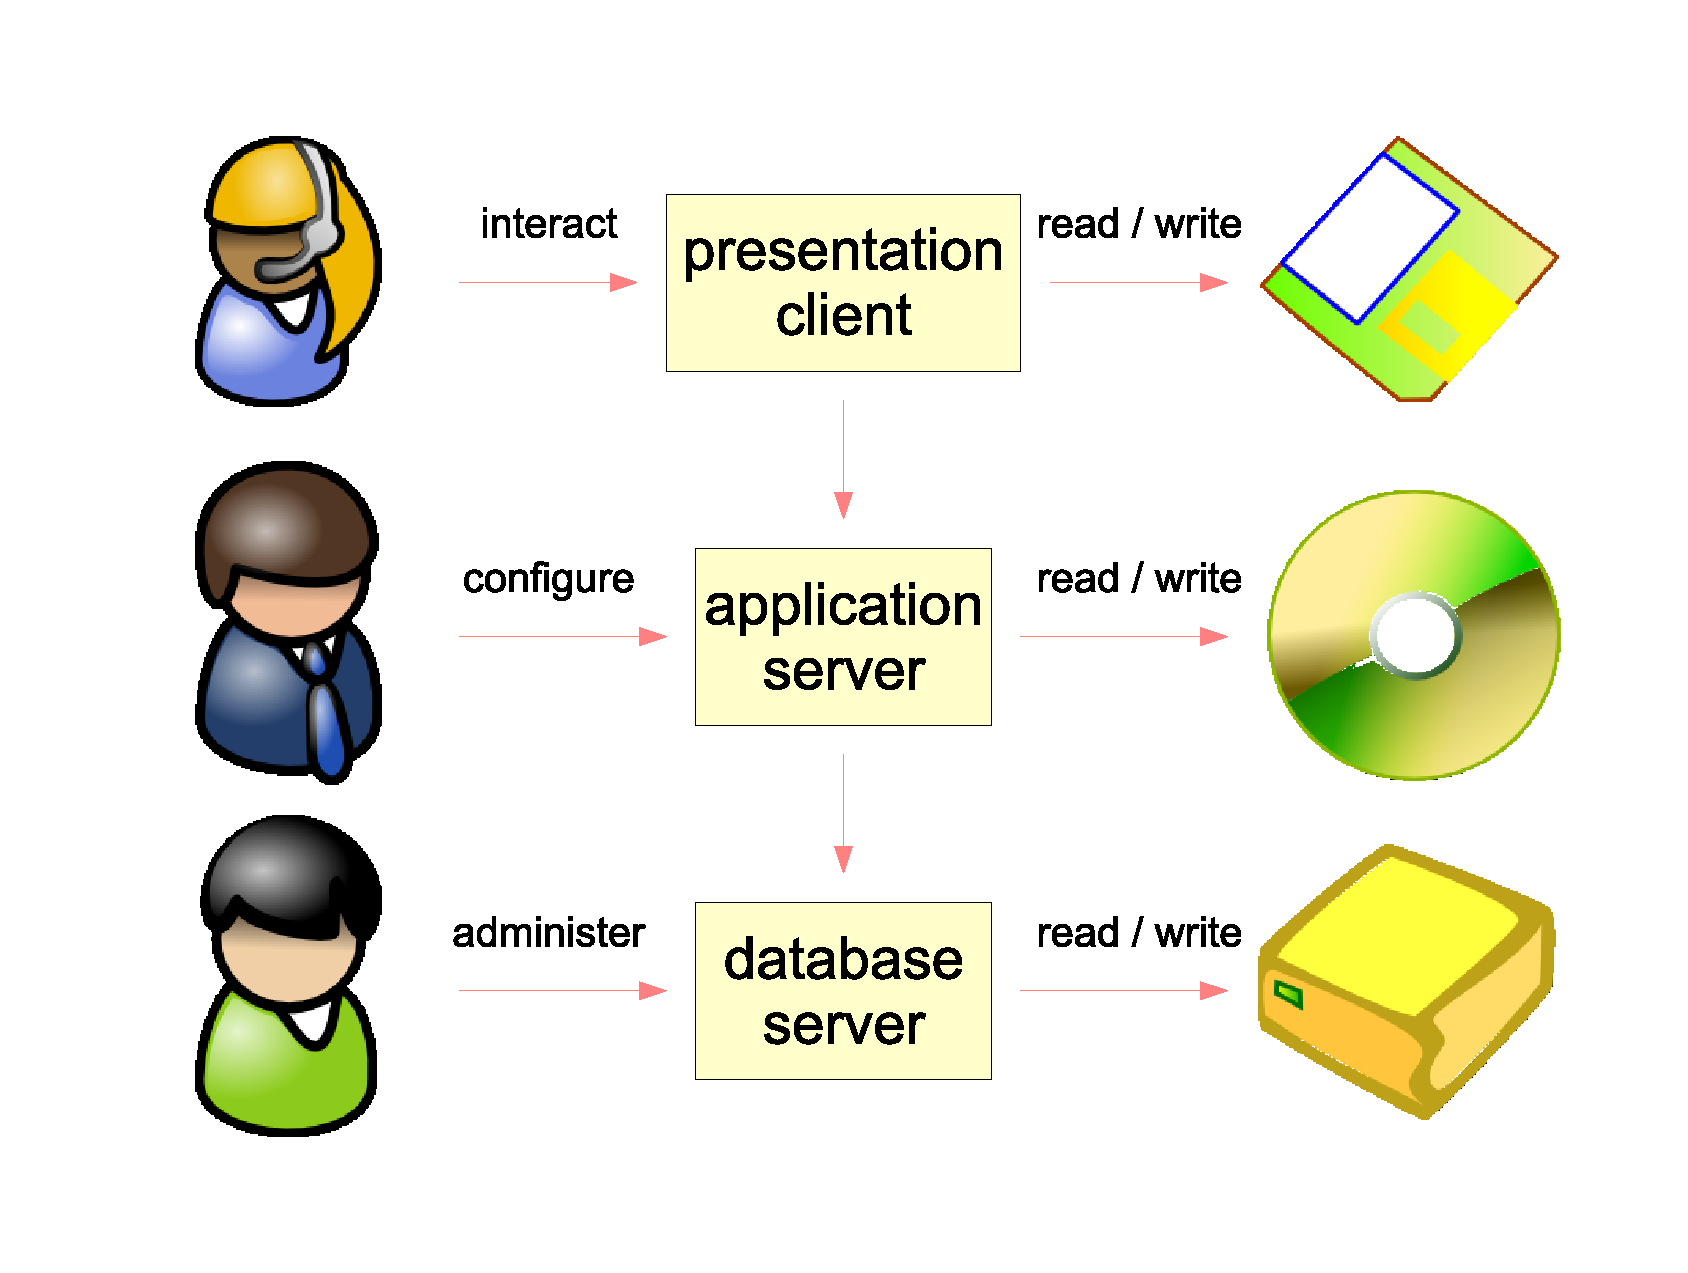
\includegraphics[scale=0.2]{vector/universal.eps}
        \caption{Universal Communication}
        \label{universal_figure}
    \end{center}
\end{figure}

Figure \ref{universal_figure} shows a three-tier environment: tier 1 represents
the \emph{Presentation Layer}; tier 2 stands for the \emph{Application Layer};
tier 3 is the \emph{Database (DB) Layer}. Typical synonyms are, in this order:
\emph{Frontend}, \emph{Business Logic} and \emph{Backend}. The tiers (layers)
serve two needs: connect different locations and share work load (\emph{Scaling}).
However, the split into tiers of that kind raises two illusions:

\begin{enumerate}
    \item \emph{Users only interact with clients}
    \item \emph{Persistent data are stored in DB only}
\end{enumerate}

Many IT architectures, or at least their illustrations, neglect the fact that
in reality \emph{all} systems need a \emph{User Interface} (UI), for at least
being administered by humans, and \emph{almost} all systems, even
\emph{Database Management Systems} (DBMS) themselves, store some of their
persistent data outside a database, for example locally available configuration
information. This is not necessarily a problem for the IT environment as such,
but it is for the internal architecture of software systems. Special solutions
have to deal with frontend (UI framework), business logic (domain patterns) and
backend (data mapping), and often additional mechanisms for local and remote
communication. The serious differences in these design solutions are one root
of well-known problems like multi- directional inter-dependencies between system
parts, that make software difficult to develop and hard to maintain.

One aim of the work described in this article was to investigate possibilities
for a \emph{unification} of communication paradigms, that is high-level design
paradigms rather than low-level protocols, in order to architect software in a
way that allows the computer system it runs on to communicate \emph{universally}.

%
% $RCSfile: modelling_mistakes.tex,v $
%
% Copyright (c) 2005-2006. Christian Heller. All rights reserved.
%
% Permission is granted to copy, distribute and/or modify this document
% under the terms of the GNU Free Documentation License, Version 1.1 or
% any later version published by the Free Software Foundation; with no
% Invariant Sections, with no Front-Cover Texts and with no Back-Cover
% Texts. A copy of the license is included in the section entitled
% "GNU Free Documentation License".
%
% http://www.cybop.net
% - Cybernetics Oriented Programming -
%
% http://www.resmedicinae.org
% - Information in Medicine -
%
% Version: $Revision: 1.1 $ $Date: 2006-01-03 08:21:45 $ $Author: christian $
% Authors: Christian Heller <christian.heller@tuxtax.de>
%

\subsection{Modelling Mistakes}
\label{modelling_mistakes_heading}

Most modern software is not written directly in a machine language but designed
in form of higher-level models instead. These allow to speed up application
development and help avoiding errors. \emph{Object Oriented Programming} (OOP),
for example, uses design concepts like the \emph{Class} owning \emph{Attributes}
and \emph{Methods}. Yet does this kind of modelling create abstractions that
reflect concepts of the real world completely and correctly?

\begin{figure}[ht]
    \begin{center}
        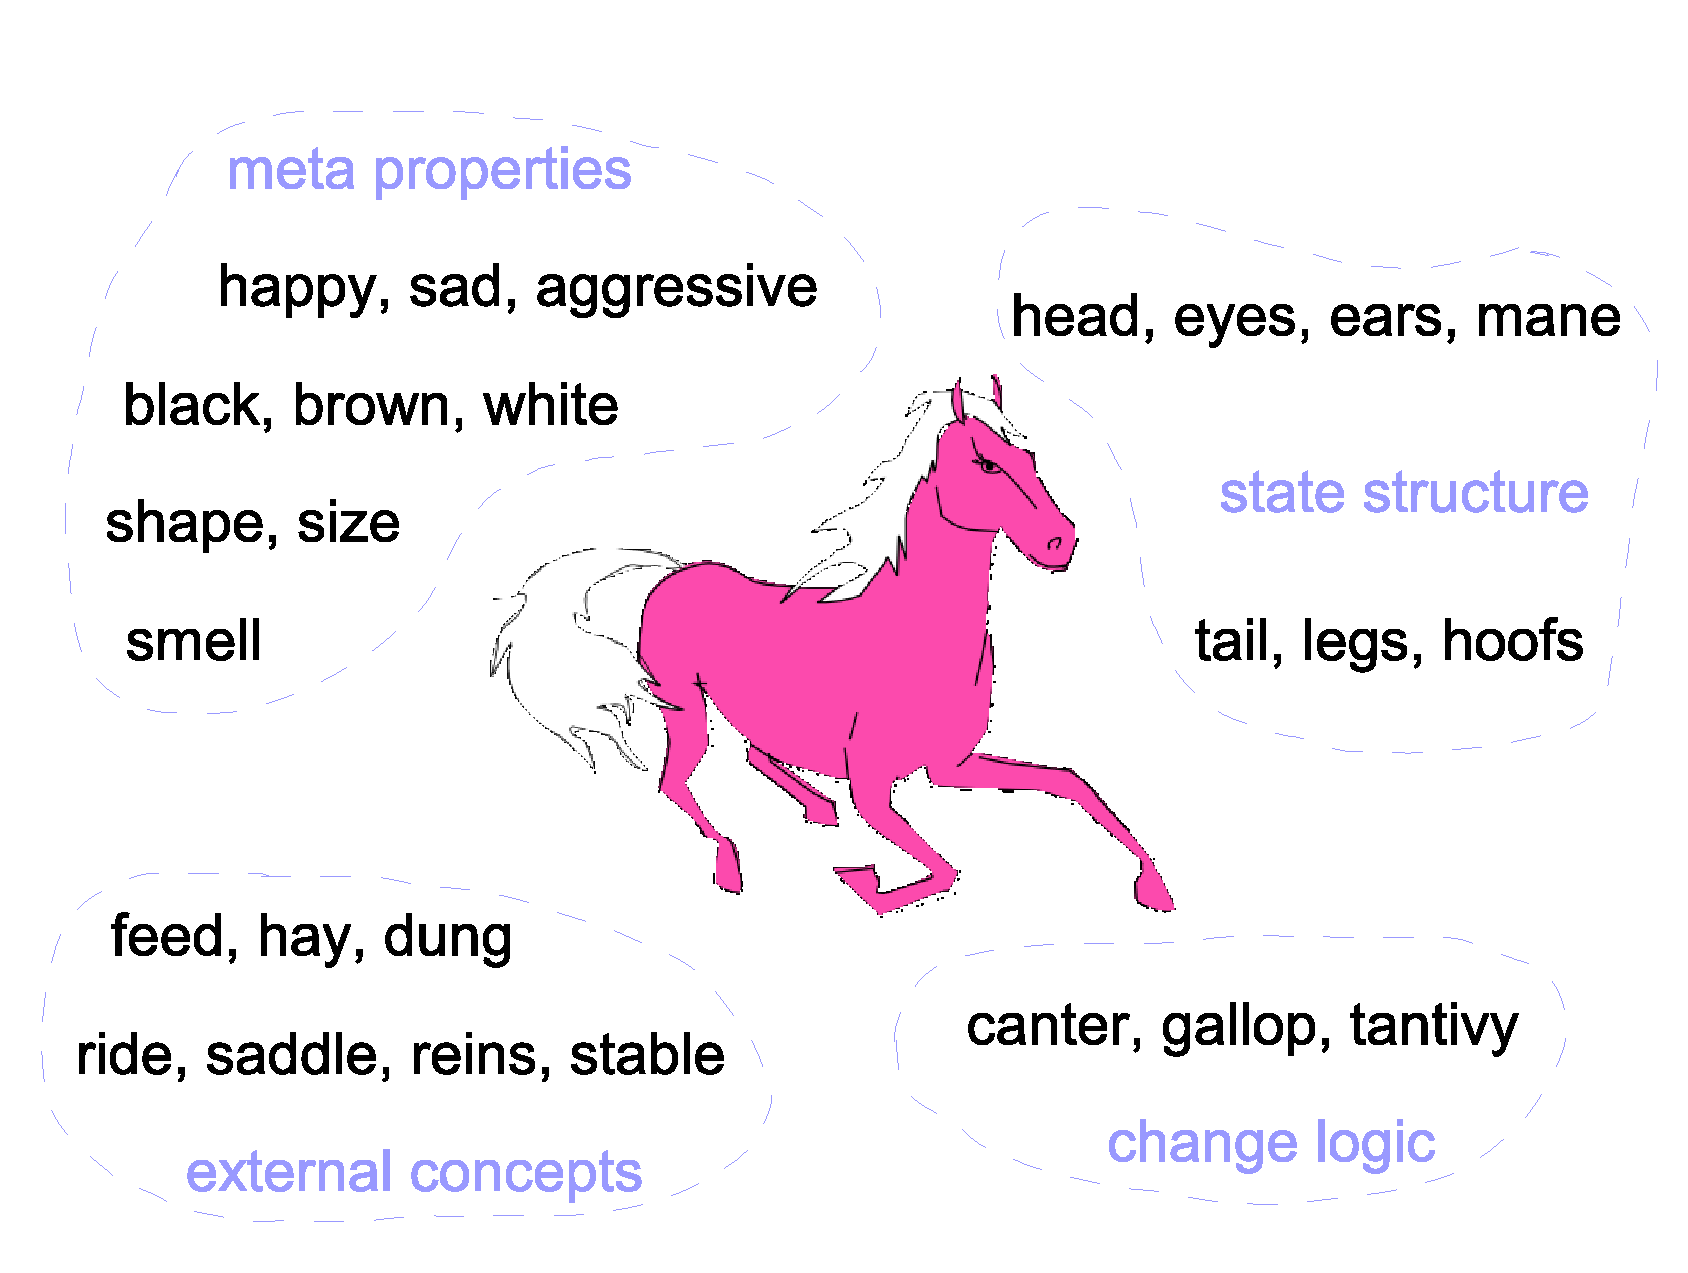
\includegraphics[scale=0.2]{vector/horse.eps}
        \caption{Concept of a Horse}
        \label{horse_figure}
    \end{center}
\end{figure}

The model of a \emph{Horse} shall serve as example to investigate this further.
Figure \ref{horse_figure} shows a number of terms commonly used to describe a
horse. Most importantly, there are structural observations describing the horse
as concept consisting of parts like \emph{Head}, \emph{Legs} or \emph{Hoofs}.
Secondly, there are properties like the horse's \emph{Colour}, \emph{Shape} or
\emph{Size}. Thirdly, there are terms describing a horse's actions like its
\emph{Movement} or \emph{Eating}, that change a horse's position and/ or state.
Finally, there are a number of terms like \emph{Hay} or \emph{Saddle}
associating concepts related to the horse.

One might suggest to model properties like the position, size or colour of a
horse's leg as \emph{Part} of that leg. In fact, this is how classical
programming approaches its solutions. In OOP, one would probably use a class
representing the leg and an attribute standing for the leg's colour. However,
when following the modelling principles of human thinking (see
\cite{heller2004}), this is \emph{not} correct!

It is true that in everyday language, one tends to say \textit{A horse leg
\emph{has a} colour.} Unfortunately, this leads to the wrong assumption that a
leg were made of a colour. But this is not the case. A leg does not
\emph{consist} of a colour in the hierarchical meaning of a whole consisting of
parts. The colour is rather property information \emph{about} the leg. It seems
there is no correct expression in natural (English) language stating the
property of something. The \emph{IS-A} verbalisation is used to express that
the leg belongs to a special category of items, for example: \textit{A leg is a
body element.} The \emph{HAS-A} formulation is used to express that a leg as
whole consists of smaller parts, for example: \textit{A leg has a knee and it
has a hoof.} But which formulation expresses a property? Well, perhaps it would
be best to say: \textit{A leg IS-OF a colour.}

The CYBOP knowledge schema described later in this article distinguishes
structural- from meta information. Actions (like the gallop of a horse) causing
change in the model or its environment are called \emph{Logic} in this work,
since they follow certain rules.


    %
% $RCSfile: architectural_troubles.tex,v $
%
% Copyright (c) 2005-2006. Christian Heller. All rights reserved.
%
% Permission is granted to copy, distribute and/or modify this document
% under the terms of the GNU Free Documentation License, Version 1.1 or
% any later version published by the Free Software Foundation; with no
% Invariant Sections, with no Front-Cover Texts and with no Back-Cover
% Texts. A copy of the license is included in the section entitled
% "GNU Free Documentation License".
%
% http://www.cybop.net
% - Cybernetics Oriented Programming -
%
% http://www.resmedicinae.org
% - Information in Medicine -
%
% Version: $Revision: 1.1 $ $Date: 2006-01-03 08:21:45 $ $Author: christian $
% Authors: Christian Heller <christian.heller@tuxtax.de>
%

\section{Architectural Troubles}
\label{architectural_troubles_heading}

The conceptual mistakes mentioned in section \ref{introduction_heading} are
partly the reason for, and partly they are caused by incomplete programming
paradigms. Of the three abstraction principles of human thinking described in
\cite{heller2004}, OOP implements \emph{Discrimination} and
\emph{Categorisation} only. \emph{Composition} as third kind of abstraction
leading to hierarchical (tree-like) models, is not considered.

Hierarchies are not new, they are present in many ways in today's programming.
There are object hierarchies, process hierarchies, design patterns modelling a
hierarchy and more. But: the hierarchy as concept is not \emph{inherent} in the
type system of current programming languages. If it were, then \emph{every}
type would be a \emph{Container} by default. Section
\ref{inter-disciplinary_ideas_heading} will introduce such a universal type.

Yet what are the results of that incomplete type system? First and foremost,
it is the reason for the existence of multiple kinds of container types, and
therewith the reason for falsified contents when using container inheritance,
as demonstrated in \cite{javaiaq}. The lack of a general, container-like type
leads to many strong dependencies, which could be avoided when holding type
attributes as neutral elements. The language and interpreter of this work use
just one structure for knowledge representation, that covers many of the
traditional forms of containers.

Further, the bundling of attributes and methods in an OOP class forces classes
to not only relate to other classes for accessing their attributes, but also
for using the methods offered by them. This often leads to unfavourable
bidirectional dependencies \cite{heller2005}, that many software patterns even
use on purpose (which is a mistake, however \cite{heller2005}). A related
problem is that, despite multiple relations in a huge class framework, it is
often difficult or impossible to reach some instances along normal object
associations, which necessitates the introduction of statically (globally)
accessible parts, with all disadvantages \cite{heller2005}. The knowledge\\
schema introduced later on allows to build models with unidirectional relations
only, that are easy to navigate, without global access.

Other software design solutions like \emph{Concern} interfaces used in
\emph{Component Oriented Programming} (COP) \cite{avalon} or the
\emph{Join Point Model} (JPM) known from \emph{Aspect Oriented Programming}
(AOP) \cite{aspectj} have their own drawbacks. Concerns spread functionality
and cause redundant code through overlapping interfaces \cite{heller2002},
which would be avoidable using an ontological architecture \cite{hellerkunze}.
The JPM contains some unsolved issues, pointed out by \cite{huttenhuis}. Models
as proposed in this article are ontologies.

\emph{System Family Engineering} applies a so-called \emph{Six-Pack} approach
\cite{domainengg, esaps}, based on the separation of \emph{Domain Engineering}
(DE) and \emph{Application Engineering} (AE). The work described in this
article proposes a separation of knowledge and system control.

    %
% $RCSfile: approach.tex,v $
%
% Copyright (c) 2005-2006. Christian Heller. All rights reserved.
%
% Permission is granted to copy, distribute and/or modify this document
% under the terms of the GNU Free Documentation License, Version 1.1 or
% any later version published by the Free Software Foundation; with no
% Invariant Sections, with no Front-Cover Texts and with no Back-Cover
% Texts. A copy of the license is included in the section entitled
% "GNU Free Documentation License".
%
% http://www.cybop.net
% - Cybernetics Oriented Programming -
%
% http://www.resmedicinae.org
% - Information in Medicine -
%
% Version: $Revision: 1.1 $ $Date: 2006-01-03 08:21:45 $ $Author: christian $
% Authors: Christian Heller <christian.heller@tuxtax.de>
%

\section{Approach}
\label{approach_heading}

On its way to solving the issues mentioned in sections
\ref{introduction_heading} and \ref{architectural_troubles_heading}, the
work followed the \emph{Cybernetics Oriented Programming} (CYBOP) approach
\cite{heller2004}. The idea behind is as simple as it is helpful; it suggests
to:

\begin{center}
    Inspect solutions of various disciplines\\
    of science, phenomenons of nature,\\
    and apply them to software engineering.
\end{center}

Figure \ref{mindmap_figure} shows some sciences whose principles were
considered in this work. The name of a field of science is shown on top of each
box. Made observations are mentioned below, in the middle. The resulting design
recommendations for software can be found at the bottom of each box. The
recommendations are grouped into those that justify a distinction between
\emph{Statics and Dynamics}, a new kind of \emph{Knowledge Schema} and a
separation of \emph{State- and Logic} models.

\begin{figure}[ht]
    \begin{center}
        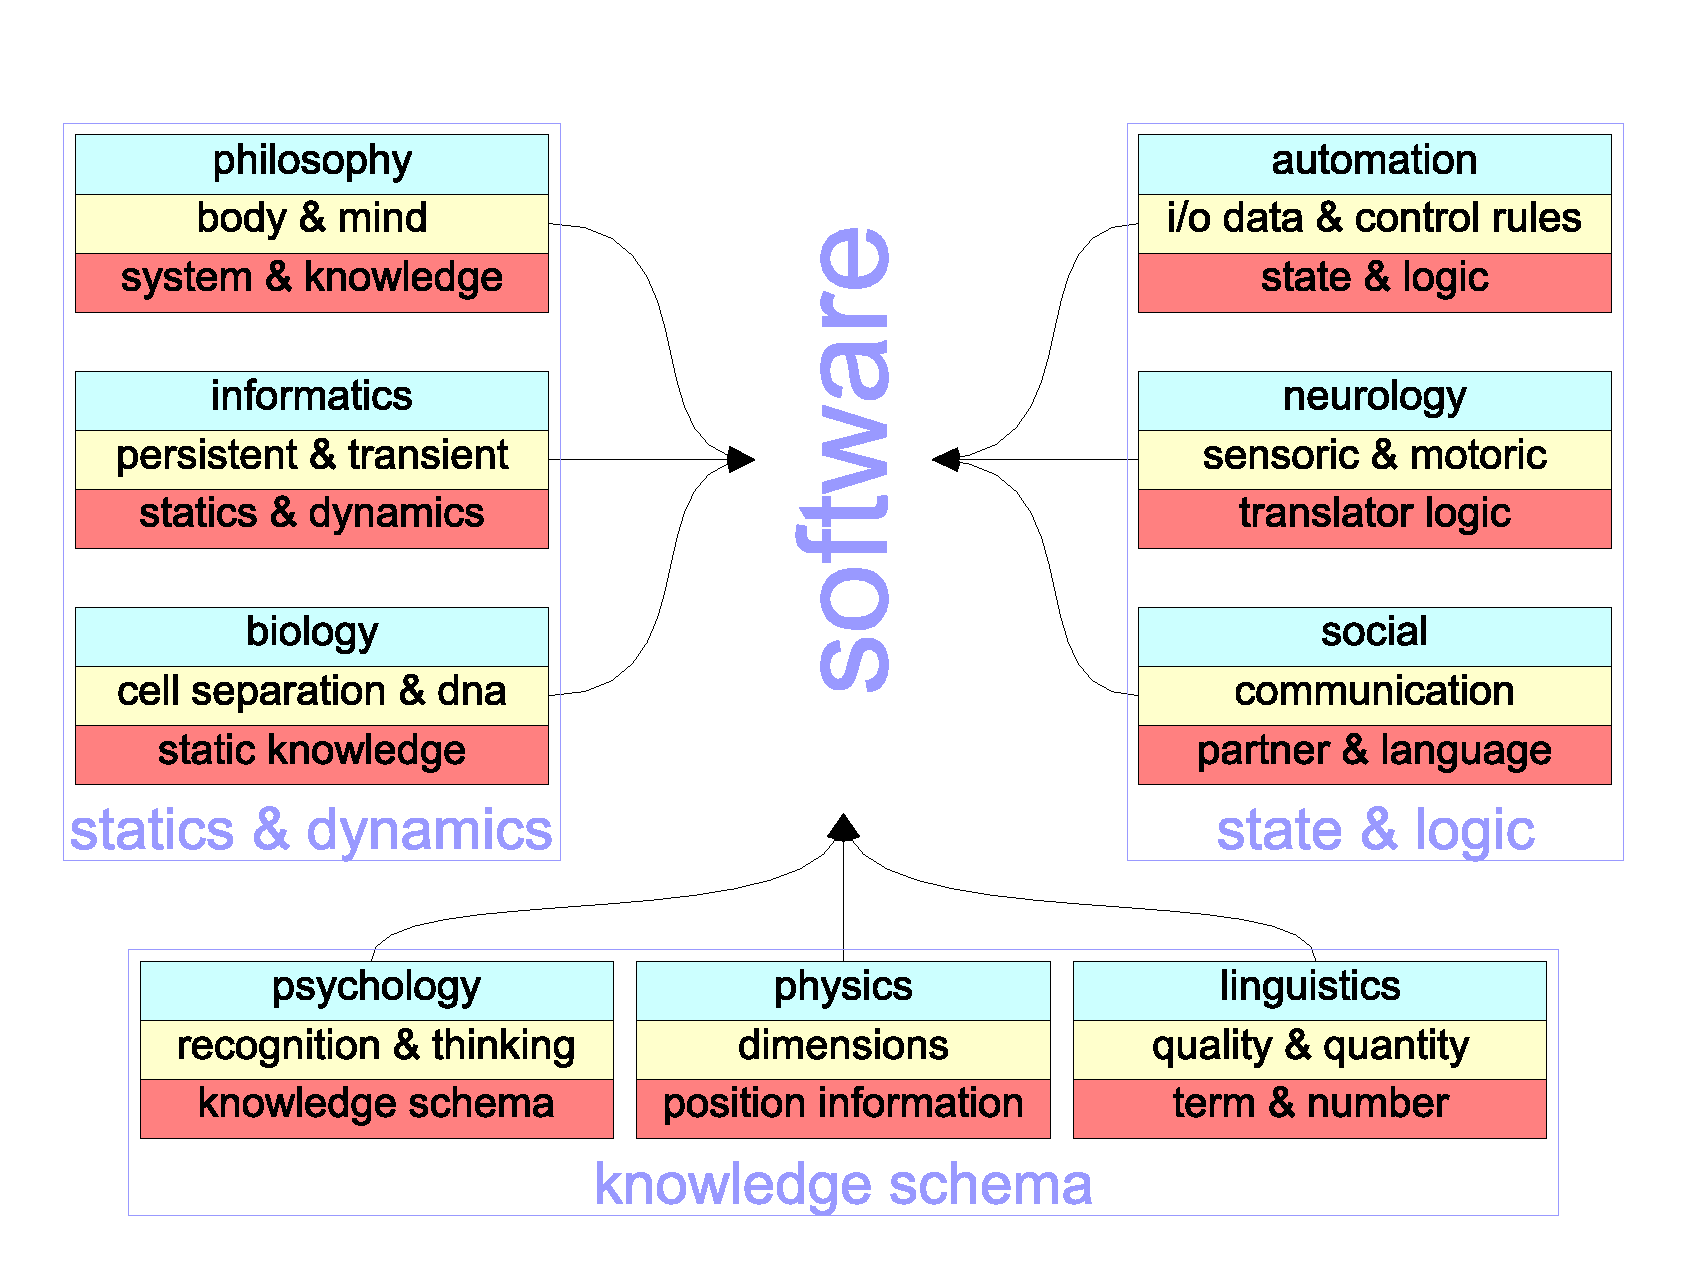
\includegraphics[scale=0.2]{vector/mindmap.eps}
        \caption{Mindmap of Influential Sciences}
        \label{mindmap_figure}
    \end{center}
\end{figure}

\begin{figure}[ht]
    \begin{center}
        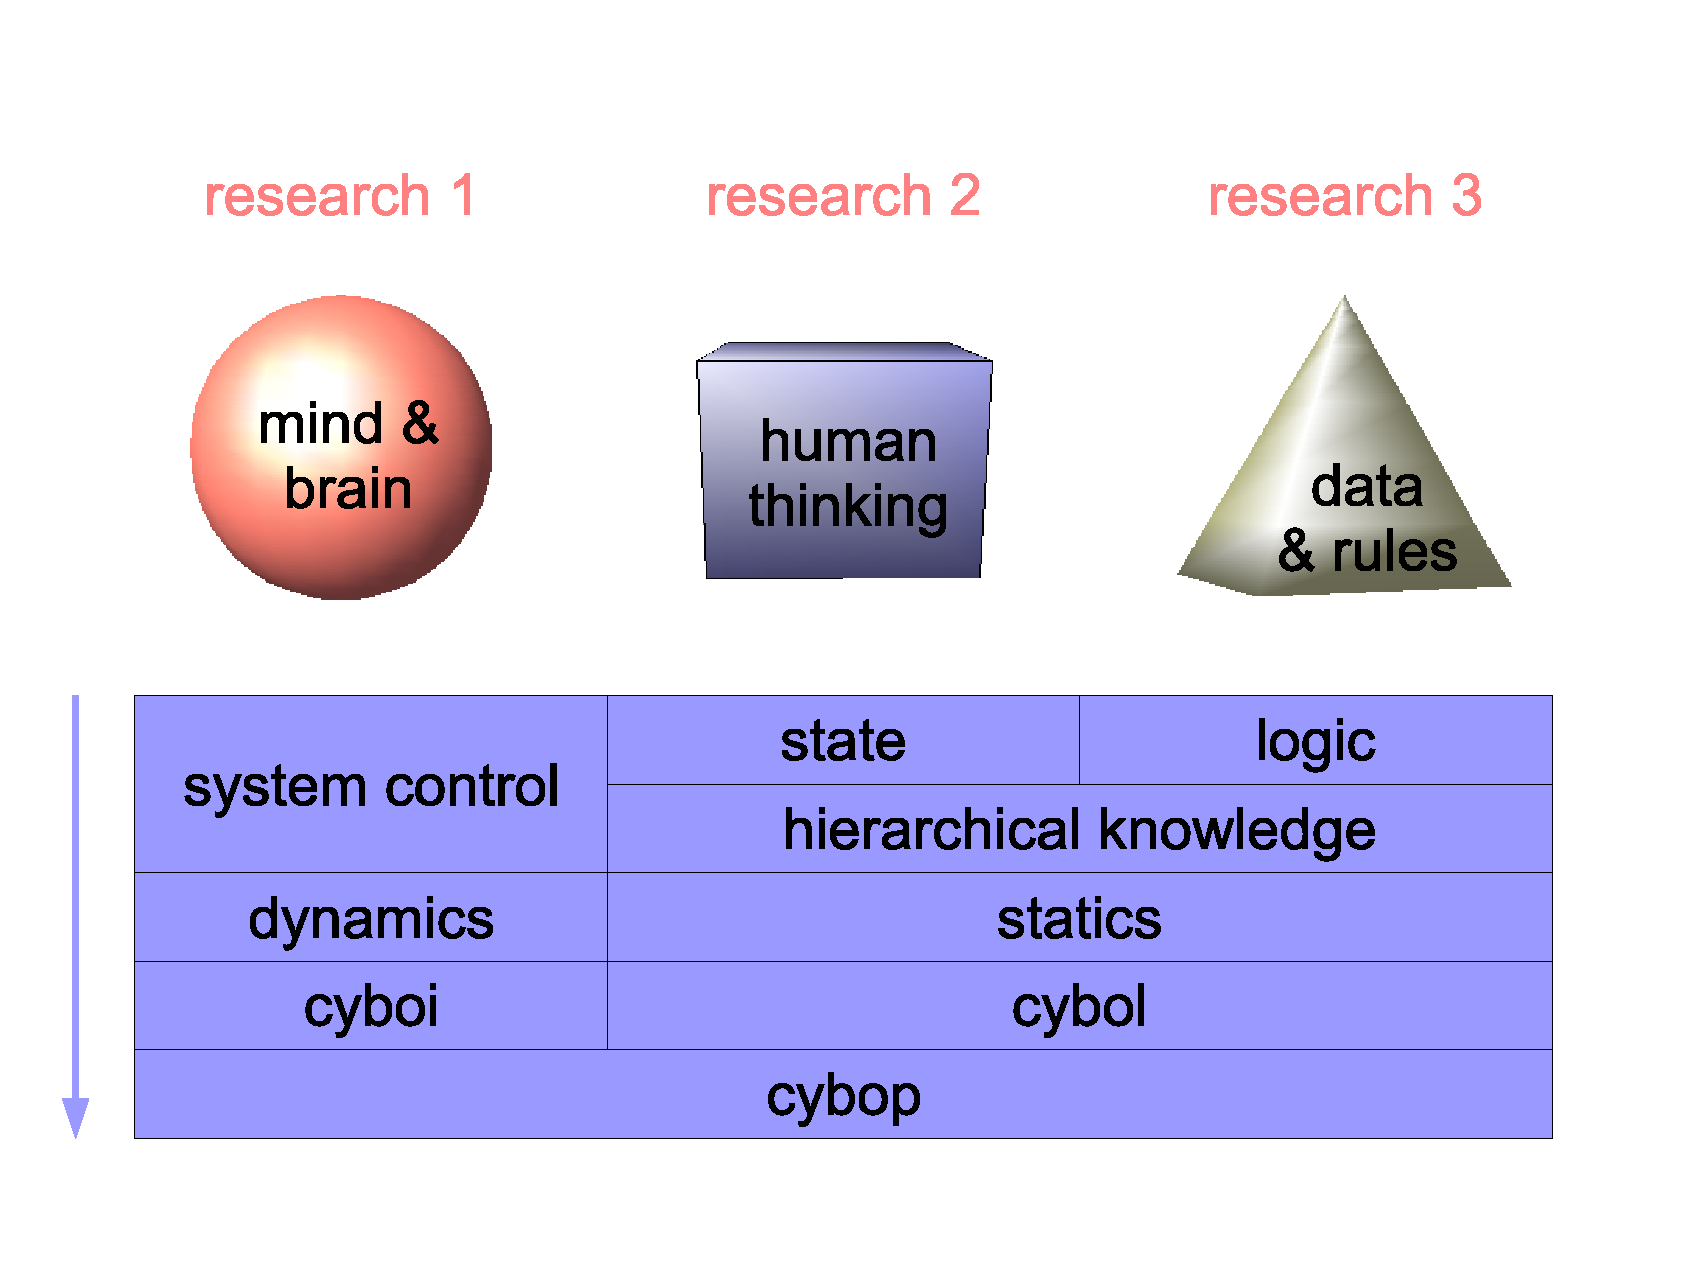
\includegraphics[scale=0.2]{vector/approach.eps}
        \caption{Overall CYBOP Approach}
        \label{approach_figure}
    \end{center}
\end{figure}

A first observation, when looking at human beings from a philosophical
perspective, is the separation of \emph{Mind} and \emph{Brain} (Body).
Accordingly, CYBOP treats computers as \emph{Systems} owning and processing
\emph{Knowledge}. This is not unlike the idea of \emph{Agent} systems owning a
\emph{Knowledge Base} \cite{parks, kuehnel}. All abstract knowledge that humans
make up belongs to their mind. The brain is merely a physical carrier of
knowledge. Similarly, there are actually two kinds of software: one
representing \emph{passive} knowledge and the other \emph{actively} controlling
a system's hardware.

Secondly, attention is payed to the concepts of \emph{Human Thinking}
\cite{heller2004}, as investigated by psychology. Through their application,
knowledge becomes \emph{hierarchical}. Moreover, this work tries to embed
knowledge models in an environment of \emph{Dimensions}, as known from physics.
Every model keeps a number of \emph{Meta Information} about its parts.
\emph{Positions} in space or time are one such example.

Thirdly, \emph{State-} gets distinguished from \emph{Logic} knowledge. It is
known from neurological research that the human brain has special communication
regions that, simply spoken, do nothing else than translating data, i.e. an
input- into an output \emph{State}, according to rules of \emph{Logic}. Systems
theory uses similar abstractions. When talking about states, this work means a
composed \emph{Set} of states.

In CYBOP (figure \ref{approach_figure}), all knowledge (states and logic),
belongs to a system's \emph{Statics}, and is described by CYBOL language
templates (section \ref{practical_proof_heading}). The processing of knowledge
at runtime, to control a system, is \emph{Dynamics} and happens in the CYBOI
interpreter.

    %
% $RCSfile: inter-disciplinary_ideas.tex,v $
%
% Copyright (c) 2005-2006. Christian Heller. All rights reserved.
%
% Permission is granted to copy, distribute and/or modify this document
% under the terms of the GNU Free Documentation License, Version 1.1 or
% any later version published by the Free Software Foundation; with no
% Invariant Sections, with no Front-Cover Texts and with no Back-Cover
% Texts. A copy of the license is included in the section entitled
% "GNU Free Documentation License".
%
% http://www.cybop.net
% - Cybernetics Oriented Programming -
%
% http://www.resmedicinae.org
% - Information in Medicine -
%
% Version: $Revision: 1.1 $ $Date: 2006-01-03 08:21:45 $ $Author: christian $
% Authors: Christian Heller <christian.heller@tuxtax.de>
%

\section{Inter-Disciplinary Ideas}
\label{inter-disciplinary_ideas_heading}

Many scientific fields (section \ref{approach_heading}) have been touched and
delivered ideas for this work, not all of whom can be mentioned or elaborated
in this article. A few examples shall be given, though; one for each proposal.

%
% $RCSfile$
%
% Copyright (c) 2005-2006. Christian Heller. All rights reserved.
%
% Permission is granted to copy, distribute and/or modify this document
% under the terms of the GNU Free Documentation License, Version 1.1 or
% any later version published by the Free Software Foundation; with no
% Invariant Sections, with no Front-Cover Texts and with no Back-Cover
% Texts. A copy of the license is included in the section entitled
% "GNU Free Documentation License".
%
% http://www.cybop.net
% - Cybernetics Oriented Programming -
%
% http://www.resmedicinae.org
% - Information in Medicine -
%
% Version: $Revision$ $Date$ $Author$
% Authors: Christian Heller <christian.heller@tuxtax.de>
%

\subsection{Statics and Dynamics}
\label{statics_and_dynamics_heading}

Of the many scientific fields that have been touched and delivered design
ideas for CYBOP, only few can be elaborated in this article, due to the limited
space.

%
% $RCSfile: code_reduction.tex,v $
%
% Copyright (C) 2002-2008. Christian Heller.
%
% Permission is granted to copy, distribute and/or modify this document
% under the terms of the GNU Free Documentation License, Version 1.1 or
% any later version published by the Free Software Foundation; with no
% Invariant Sections, with no Front-Cover Texts and with no Back-Cover
% Texts. A copy of the license is included in the section entitled
% "GNU Free Documentation License".
%
% http://www.cybop.net
% - Cybernetics Oriented Programming -
%
% http://www.resmedicinae.org
% - Information in Medicine -
%
% Version: $Revision: 1.1 $ $Date: 2008-08-19 20:41:05 $ $Author: christian $
% Authors: Christian Heller <christian.heller@tuxtax.de>
%

\subsection{Code Reduction}
\label{code_reduction_heading}
\index{Code Reduction}
\index{Picture Element}
\index{Pixel}

In his book \emph{Programming Pearls} \cite[page 128]{bentley}, Jon Bentley
demonstrates \emph{Code Reduction} on the following graphics program example:

\begin{scriptsize}
    \begin{verbatim}
� � for i = [17, 43] set(i, 68)
� � for i = [18, 42] set(i, 69)
� � for j = [81, 91] set(30, j)
� � for j = [82, 92] set(31, j)
    \end{verbatim}
\end{scriptsize}

He suggests to replace the \emph{set} procedures that switch a
\emph{Picture Element} (Pixel) with suitable functions for drawing horizontal
and vertical lines:

\begin{scriptsize}
    \begin{verbatim}
� � hor(17, 43, 68)
� � hor(18, 42, 69)
� � vert(81, 91, 30)
� � vert(82, 92, 31)
    \end{verbatim}
\end{scriptsize}

This code, finally, gets reduced to pure data stored in an array:

\begin{scriptsize}
    \begin{verbatim}
� � h 17 43 68
� � h 18 42 69
� � v 81 91 30
� � v 82 92 31
    \end{verbatim}
\end{scriptsize}

The data can be read by an interpreter program which knows about their meaning.

Bentley's example shows in a nice way how knowledge can be extracted from program
source code. The graphic application's actual data are represented by the values
in the array above. All other functionality accessing and manipulating Pixels
directly does belong to system control and remains in the interpreter program.
Chapter \ref{cybernetics_oriented_interpreter_heading} will introduce an
interpreter that is able to read and handle \emph{general} knowledge, only on a
much larger scale.

%
% $RCSfile: base_and_meta_level.tex,v $
%
% Copyright (C) 2002-2008. Christian Heller.
%
% Permission is granted to copy, distribute and/or modify this document
% under the terms of the GNU Free Documentation License, Version 1.1 or
% any later version published by the Free Software Foundation; with no
% Invariant Sections, with no Front-Cover Texts and with no Back-Cover
% Texts. A copy of the license is included in the section entitled
% "GNU Free Documentation License".
%
% http://www.cybop.net
% - Cybernetics Oriented Programming -
%
% http://www.resmedicinae.org
% - Information in Medicine -
%
% Version: $Revision: 1.1 $ $Date: 2008-08-19 20:41:05 $ $Author: christian $
% Authors: Christian Heller <christian.heller@tuxtax.de>
%

\subsection{Base- and Meta Level}
\label{base_and_meta_level_heading}
\index{Base Level}
\index{Meta Level}
\index{Reflective Technique}
\index{System- and Application Functionality}
\index{Bidirectional Dependency}

Reflective techniques as described in section \ref{reflection_heading} make use
of one so-called \emph{Base Level} and one or more \emph{Meta Levels}. The
reason for splitting a system's architecture in this way is the hope to be able
to move rather general \emph{System Functionality} into a meta level, while
leaving domain-specific \emph{Application Functionality} in the base level.
(Well, in his book \emph{Analysis Patterns -- Reusable Object Models}
\cite{fowler1997}, Fowler used meta levels to model general classes containing
not exclusively system- but also domain-specific functionality.) The conflicts
a design decision of that kind can bring with were described in section
\ref{broken_type_system_heading}, which -- above all -- criticised the
bidirectional dependencies.

However, what the proposition of reflective software patterns shows, is the
existence of a wish among software developers, to separate general system- from
more specific application functionality. And, as was shown in section
\ref{virtual_and_real_world_heading}, nature does exactly that. Yet while
reflective mechanisms use the same implementation techniques for system- as
well as for application-specific functionality, nature always treats passive
knowledge strictly separate from active system control (section
\ref{virtual_and_real_world_heading}). Bidirectional dependencies do not exist
between the both.

%
% $RCSfile$
%
% Copyright (c) 2005-2006. Christian Heller. All rights reserved.
%
% Permission is granted to copy, distribute and/or modify this document
% under the terms of the GNU Free Documentation License, Version 1.1 or
% any later version published by the Free Software Foundation; with no
% Invariant Sections, with no Front-Cover Texts and with no Back-Cover
% Texts. A copy of the license is included in the section entitled
% "GNU Free Documentation License".
%
% http://www.cybop.net
% - Cybernetics Oriented Programming -
%
% http://www.resmedicinae.org
% - Information in Medicine -
%
% Version: $Revision$ $Date$ $Author$
% Authors: Christian Heller <christian.heller@tuxtax.de>
%

\subsubsection{Application and Domain}
\label{application_and_domain_heading}

Over the years, it has turned out to be helpful in software design, to separate
\emph{Domain Knowledge} from \emph{Application Functionality}. In
one-or-another form, the architectural software patterns \cite{heller2005}
\emph{Layers}, \emph{Domain Model} and \emph{Model View Controller} (MVC) all
suggest to apply this principle.

The \emph{Tools \& Materials} approach \cite{tandm} talks of \emph{active}
applications (tools) working on \emph{passive} domain data (material). And also
\emph{System Family Engineering} \cite{domainengg} bases on a separate
treatment of domain and application, in form of \emph{Domain Engineering} (DE)
and \emph{Application Engineering} (AE).

An often neglected fact of these approaches is that not only the domain, but
also the application contains important business knowledge (figure
\ref{separation_figure}). The \emph{User Interface} (UI), for example, is
tailored for a specific business domain. And the logic behind, if not
contained in the UI itself, is often put in a \emph{Controller} which belongs
to the application$-$, not the domain layer.

\begin{figure}[ht]
    \begin{center}
        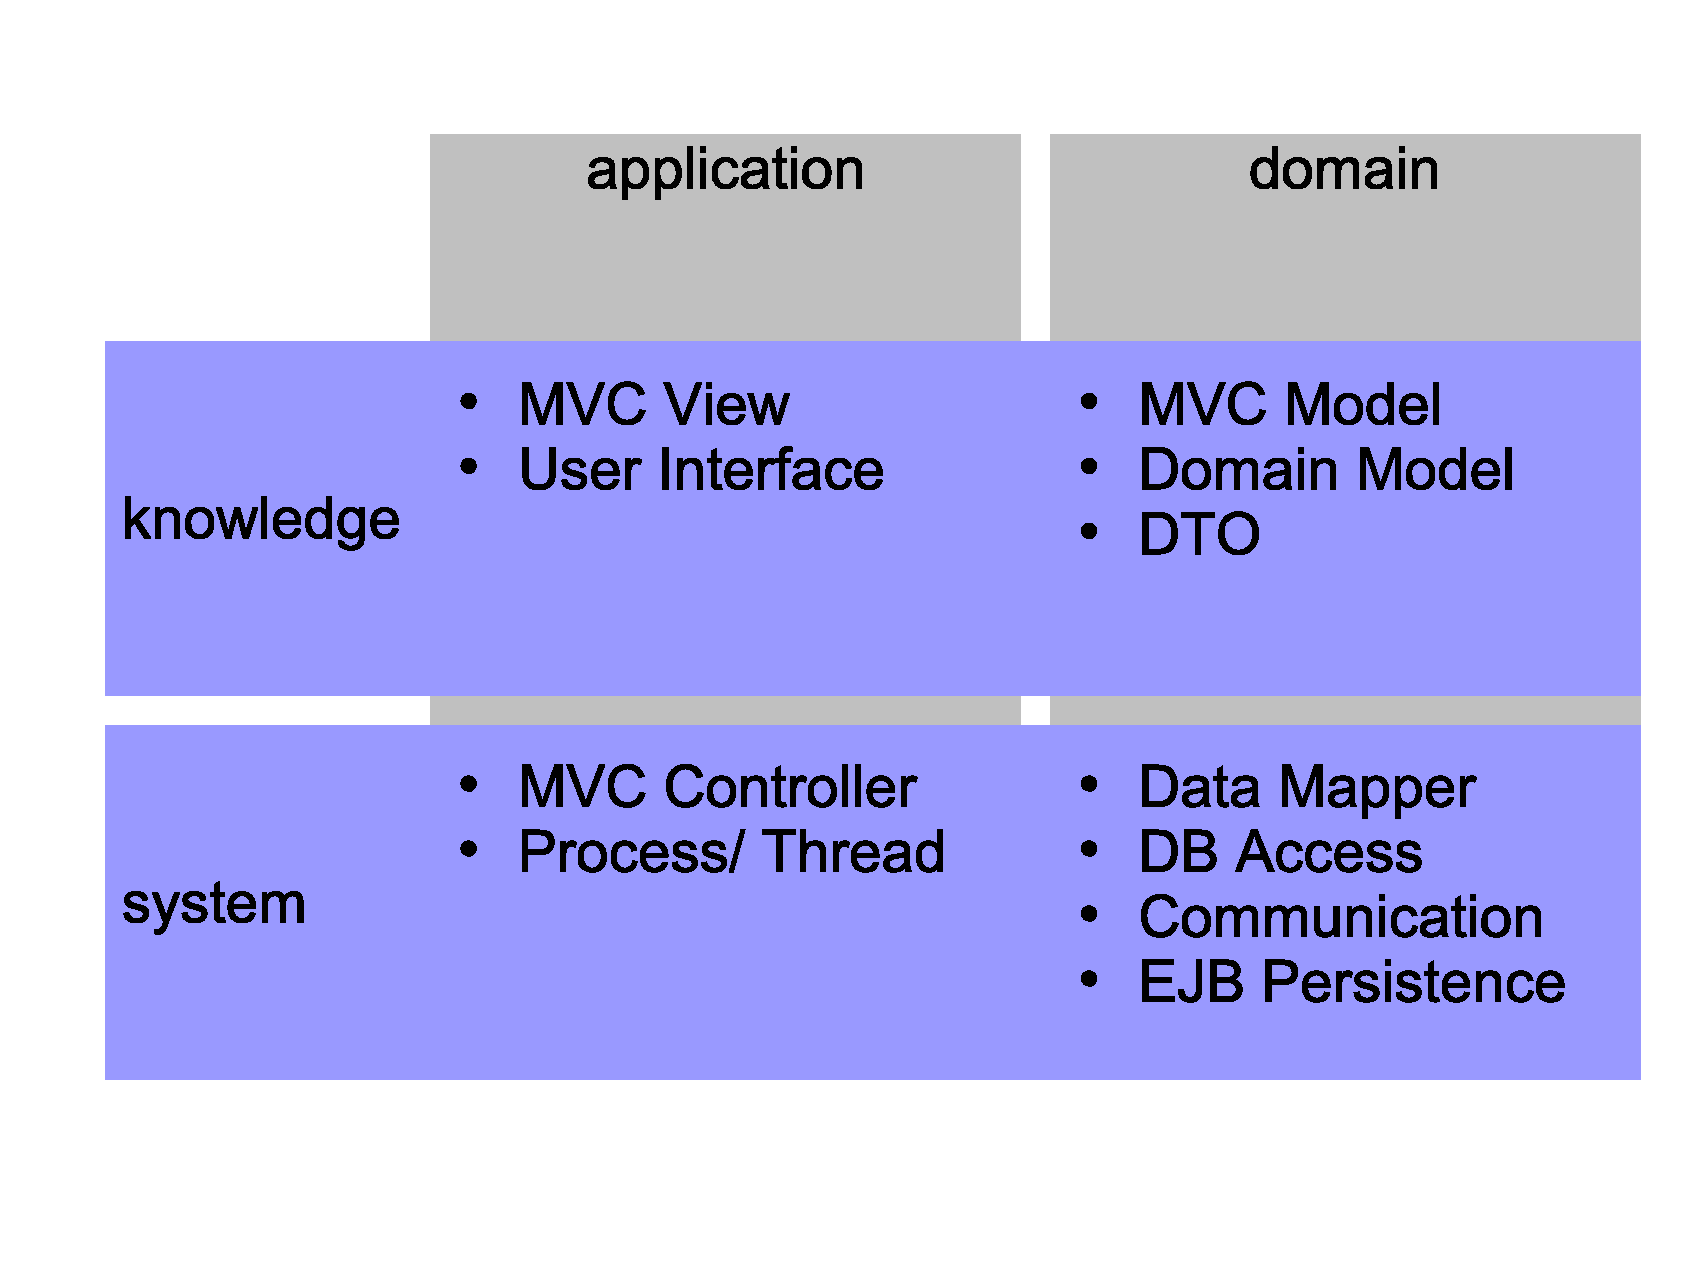
\includegraphics[scale=0.2]{vector/separation.eps}
        \caption{Different Knowledge Separations}
        \label{separation_figure}
    \end{center}
\end{figure}

Similarly, the domain often contains functionality which actually does belong
into the application process: \emph{Database} (DB) access is handled by help of
patterns like the \emph{Data Mapper} \cite{heller2005}, in which the mapper\\
objects contain \emph{Structured Query Language} (SQL) code to connect to a
\emph{Database Management System} (DBMS); \emph{Enterprise Java Beans} (EJB),
which should better be pure domain objects, imitate a \emph{Middleware}
providing persistence- or communication mechanisms, which originally have
nothing to do with the business knowledge they contain.

It is precisely this \emph{Mixup} of responsibilities between an application
system and its domain knowledge, that leads to multiple inter-dependencies and
hence unflexibility within a system. Instead, a separation should be made
between active \emph{System Control} and passive \emph{Knowledge}. A UI's
appearance would then be treated as domain knowledge, just as the logic of the
functions called through it. A data mapper would be transformed into a simple
\emph{Translator} -- similar to a \emph{Data Transfer Object} (DTO)
\cite{heller2005} -- that knows how to convert data from one domain model into
another; its DBMS access functionality, however, would be extracted and put
into the application system. Monstrosities like EJBs would likewise be opened
up and parted into their actual domain knowledge, and all other mechanisms
around -- the latter being moved into the application system.

To sum up this thought: The essential realisation here is that hardware-close
mechanisms like the ones necessary for data input/ output (i/o), enabling
inter-system communication, should be handled in an active application system
layer which was started as process on a computer, and \emph{not} be merged with
pure, passive domain knowledge. User interfaces and application logic which are
traditionally held in controller objects of the application layer, as well as
further business data models, should rather belong to a high-level knowledge
layer.

%
% $RCSfile$
%
% Copyright (c) 2002-2006. Christian Heller. All rights reserved.
%
% Permission is granted to copy, distribute and/or modify this document
% under the terms of the GNU Free Documentation License, Version 1.1 or
% any later version published by the Free Software Foundation; with no
% Invariant Sections, with no Front-Cover Texts and with no Back-Cover
% Texts. A copy of the license is included in the section entitled
% "GNU Free Documentation License".
%
% http://www.cybop.net
% - Cybernetics Oriented Programming -
%
% http://www.resmedicinae.org
% - Information in Medicine -
%
% Version: $Revision$ $Date$ $Author$
% Authors: Christian Heller <christian.heller@tuxtax.de>
%

\subsubsection{Platform Specific and -Independent}
\label{platform_specific_and_independent_heading}

The \emph{Model Driven Architecture} (MDA) \cite{mda} took a first step into
the right direction, by distinguishing \emph{Platform Independent Models}
(PIM), that is domain- and application logic, and \emph{Platform Specific Models}
(PSM), that is implementation technology. It encourages the use of automated
tools for defining and transforming these models.

While the definition, organisation and management of architectures (PIM) mostly
happen in the analysis- and design phase of a \emph{Software Engineering Process}
(SEP) (section \ref{abstraction_gaps_heading}), the generation of source code
(PSM) can be assigned to the implementation phase. The approach still has
weaknesses, and tools which can truly generate running systems are rare or not
existent, at least to what concerns more complex software systems -- not to
talk of the so-called \emph{Roundtrip Engineering}, which is managed by even
less tools.

Nevertheless, the trend clearly goes towards more model-centric approaches. The
aim of this work was to supply domain experts and application developers with a
\emph{Model Only} technology, allowing to create application systems that do
\emph{not} have to be transformed into classical implementation code any longer,
whereby the SEP abstraction gap number \emph{2} (figure \ref{gaps_figure})
could be closed conclusively. The knowledge schema introduced in section
\ref{knowledge_schema_heading} is a necessary prerequisite therefor.

%
% $RCSfile$
%
% Copyright (c) 2005-2006. Christian Heller. All rights reserved.
%
% Permission is granted to copy, distribute and/or modify this document
% under the terms of the GNU Free Documentation License, Version 1.1 or
% any later version published by the Free Software Foundation; with no
% Invariant Sections, with no Front-Cover Texts and with no Back-Cover
% Texts. A copy of the license is included in the section entitled
% "GNU Free Documentation License".
%
% http://www.cybop.net
% - Cybernetics Oriented Programming -
%
% http://www.resmedicinae.org
% - Information in Medicine -
%
% Version: $Revision$ $Date$ $Author$
% Authors: Christian Heller <christian.heller@tuxtax.de>
%

\subsubsection{Data Garden}
\label{data_garden_heading}

Now, if a distinction of high-level knowledge from low-level system control
software is considered to be useful, the next question must be: \textit{How,
that is in which form, best to store knowledge in a system?}

One possible structure called \emph{Data Garden} \cite{holland} was proposed by
Wau Holland of the \emph{Chaos Computer Club} (CCC). Although being a
non-academic organisation, his ideas on knowledge modelling are interesting to
this work. He dreamt of whole \emph{Forests}, \emph{Parks} or -- as the name
says -- \emph{Gardens} of \emph{Knowledge Trees} and \emph{Data Bushes} (figure
\ref{garden_figure}).

\begin{figure}[ht]
    \begin{center}
        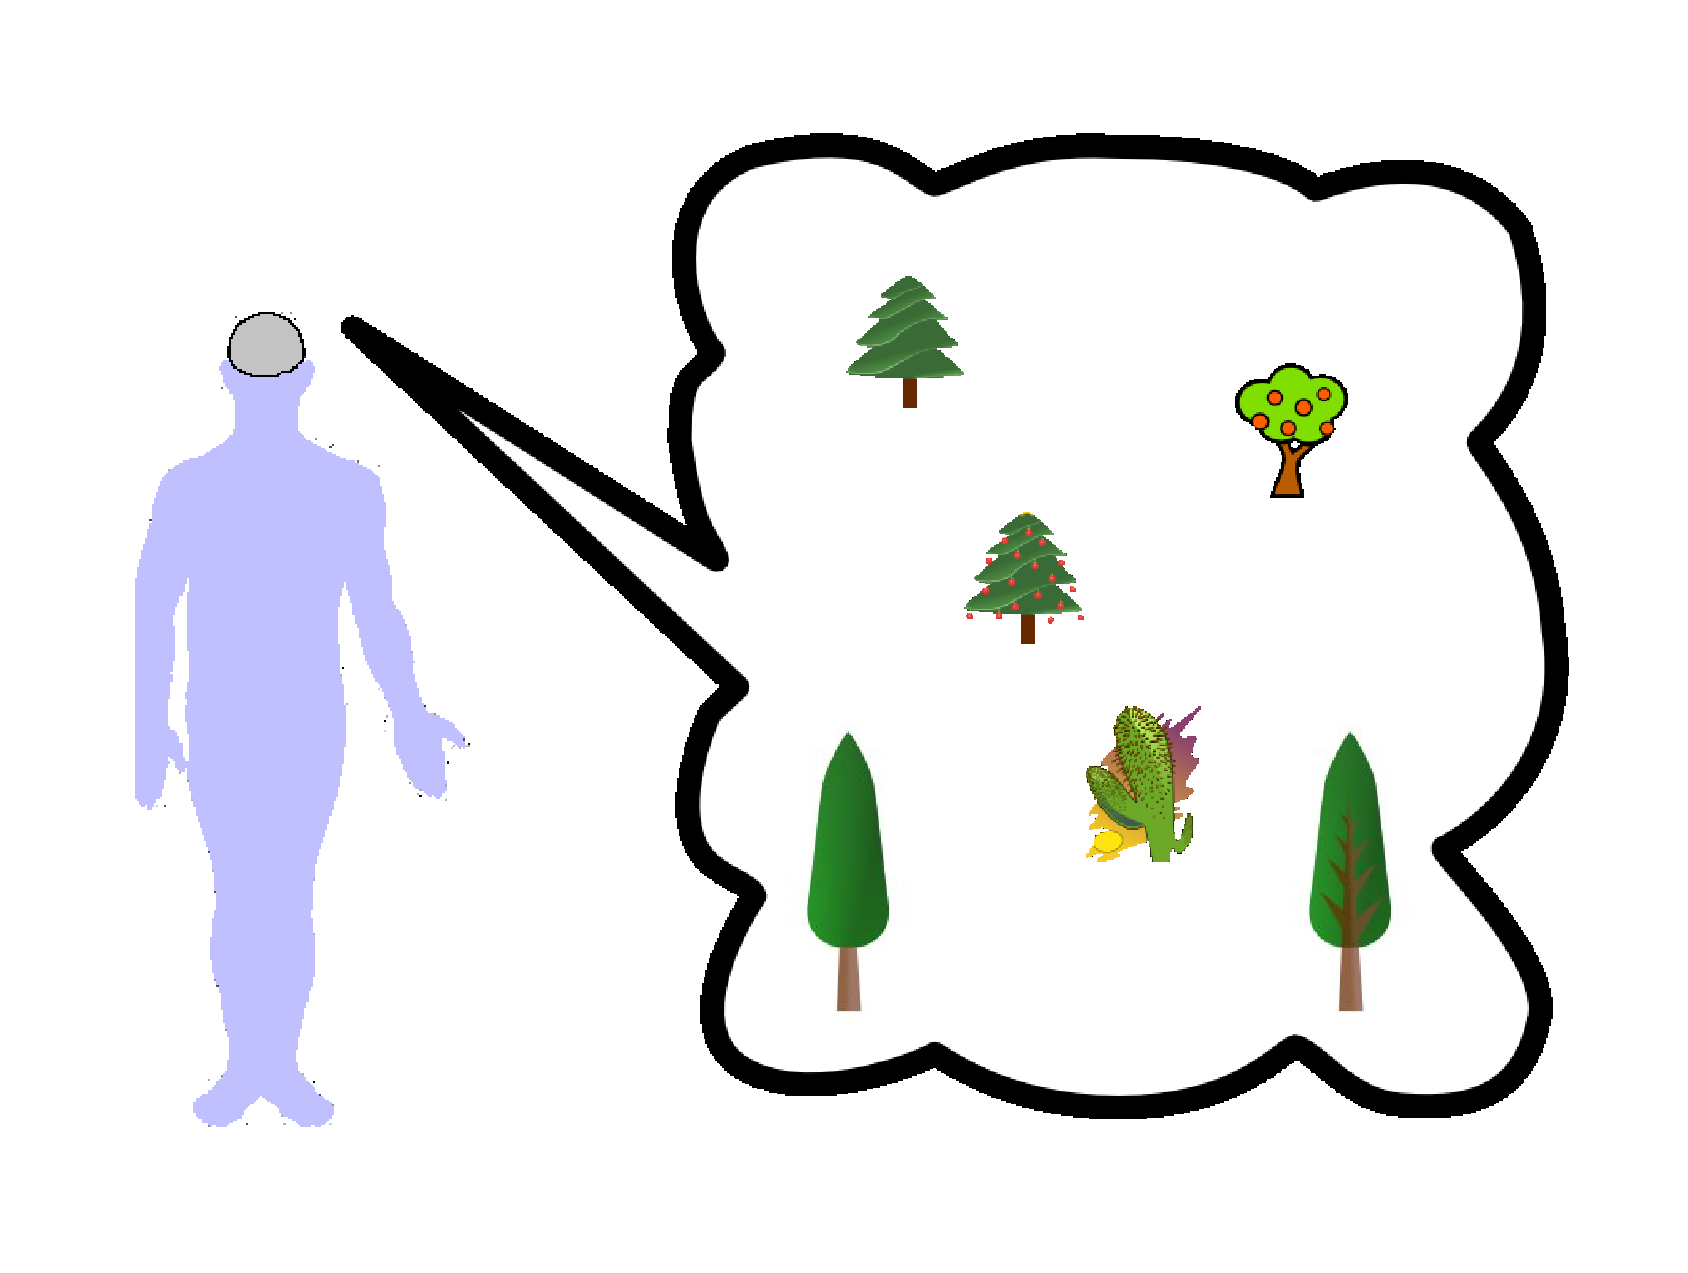
\includegraphics[scale=0.2]{vector/garden.eps}
        \caption{Data Garden}
        \label{garden_figure}
    \end{center}
\end{figure}

The interpreter (section \ref{cyboi_heading}) created in the work described in
this article stores all its knowledge in \emph{one single} tree, whose root
node it references. The single concepts (data bushes) are represented by
branches of that knowledge tree.


%
% $RCSfile$
%
% Copyright (c) 2005-2006. Christian Heller. All rights reserved.
%
% Permission is granted to copy, distribute and/or modify this document
% under the terms of the GNU Free Documentation License, Version 1.1 or
% any later version published by the Free Software Foundation; with no
% Invariant Sections, with no Front-Cover Texts and with no Back-Cover
% Texts. A copy of the license is included in the section entitled
% "GNU Free Documentation License".
%
% http://www.cybop.net
% - Cybernetics Oriented Programming -
%
% http://www.resmedicinae.org
% - Information in Medicine -
%
% Version: $Revision$ $Date$ $Author$
% Authors: Christian Heller <christian.heller@tuxtax.de>
%

\subsection{Knowledge Schema}
\label{knowledge_schema_heading}

Human beings have a brain which they use to think, in other words to build up a
mind. While the former exists in the \emph{Real World}, the latter is
constructed as a subjective \emph{Virtual World}. All people do think, all the
time, even not knowing that they do. One would therefore guess that the act of
\emph{Thinking} is a most common one, familiar to anybody. But judging from the
enormous research effort in sciences dealing with it, the \emph{Principles}
behind thinking are not that easy to grasp.

%
% $RCSfile: schema.tex,v $
%
% Copyright (C) 2002-2008. Christian Heller.
%
% Permission is granted to copy, distribute and/or modify this document
% under the terms of the GNU Free Documentation License, Version 1.1 or
% any later version published by the Free Software Foundation; with no
% Invariant Sections, with no Front-Cover Texts and with no Back-Cover
% Texts. A copy of the license is included in the section entitled
% "GNU Free Documentation License".
%
% http://www.cybop.net
% - Cybernetics Oriented Programming -
%
% http://www.resmedicinae.org
% - Information in Medicine -
%
% Version: $Revision: 1.1 $ $Date: 2008-08-19 20:41:08 $ $Author: christian $
% Authors: Christian Heller <christian.heller@tuxtax.de>
%

\subsection{Schema}
\label{schema_heading}
\index{Schema with Meta Information}
\index{Knowledge Schema with Meta Information}
\index{Model}
\index{Concept}
\index{Item}
\index{Category}
\index{Compound}
\index{Discrimination}
\index{Categorisation}
\index{Composition}
\index{Compound Model}
\index{Meta Information}
\index{Meta Model}

A theoretical \emph{Model} is an abstract clip of the real world, and exists in
the human mind. Another common word for \emph{Model} is \emph{Concept}. It is
the subsumption of \emph{Item}, \emph{Category} and \emph{Compound}, resulting
from three activities of abstraction: \emph{Discrimination}, \emph{Categorisation}
and \emph{Composition} (section \ref{abstraction_heading}). As such, each model
\emph{knows} about the parts it consists of.

\begin{figure}[ht]
    \begin{center}
        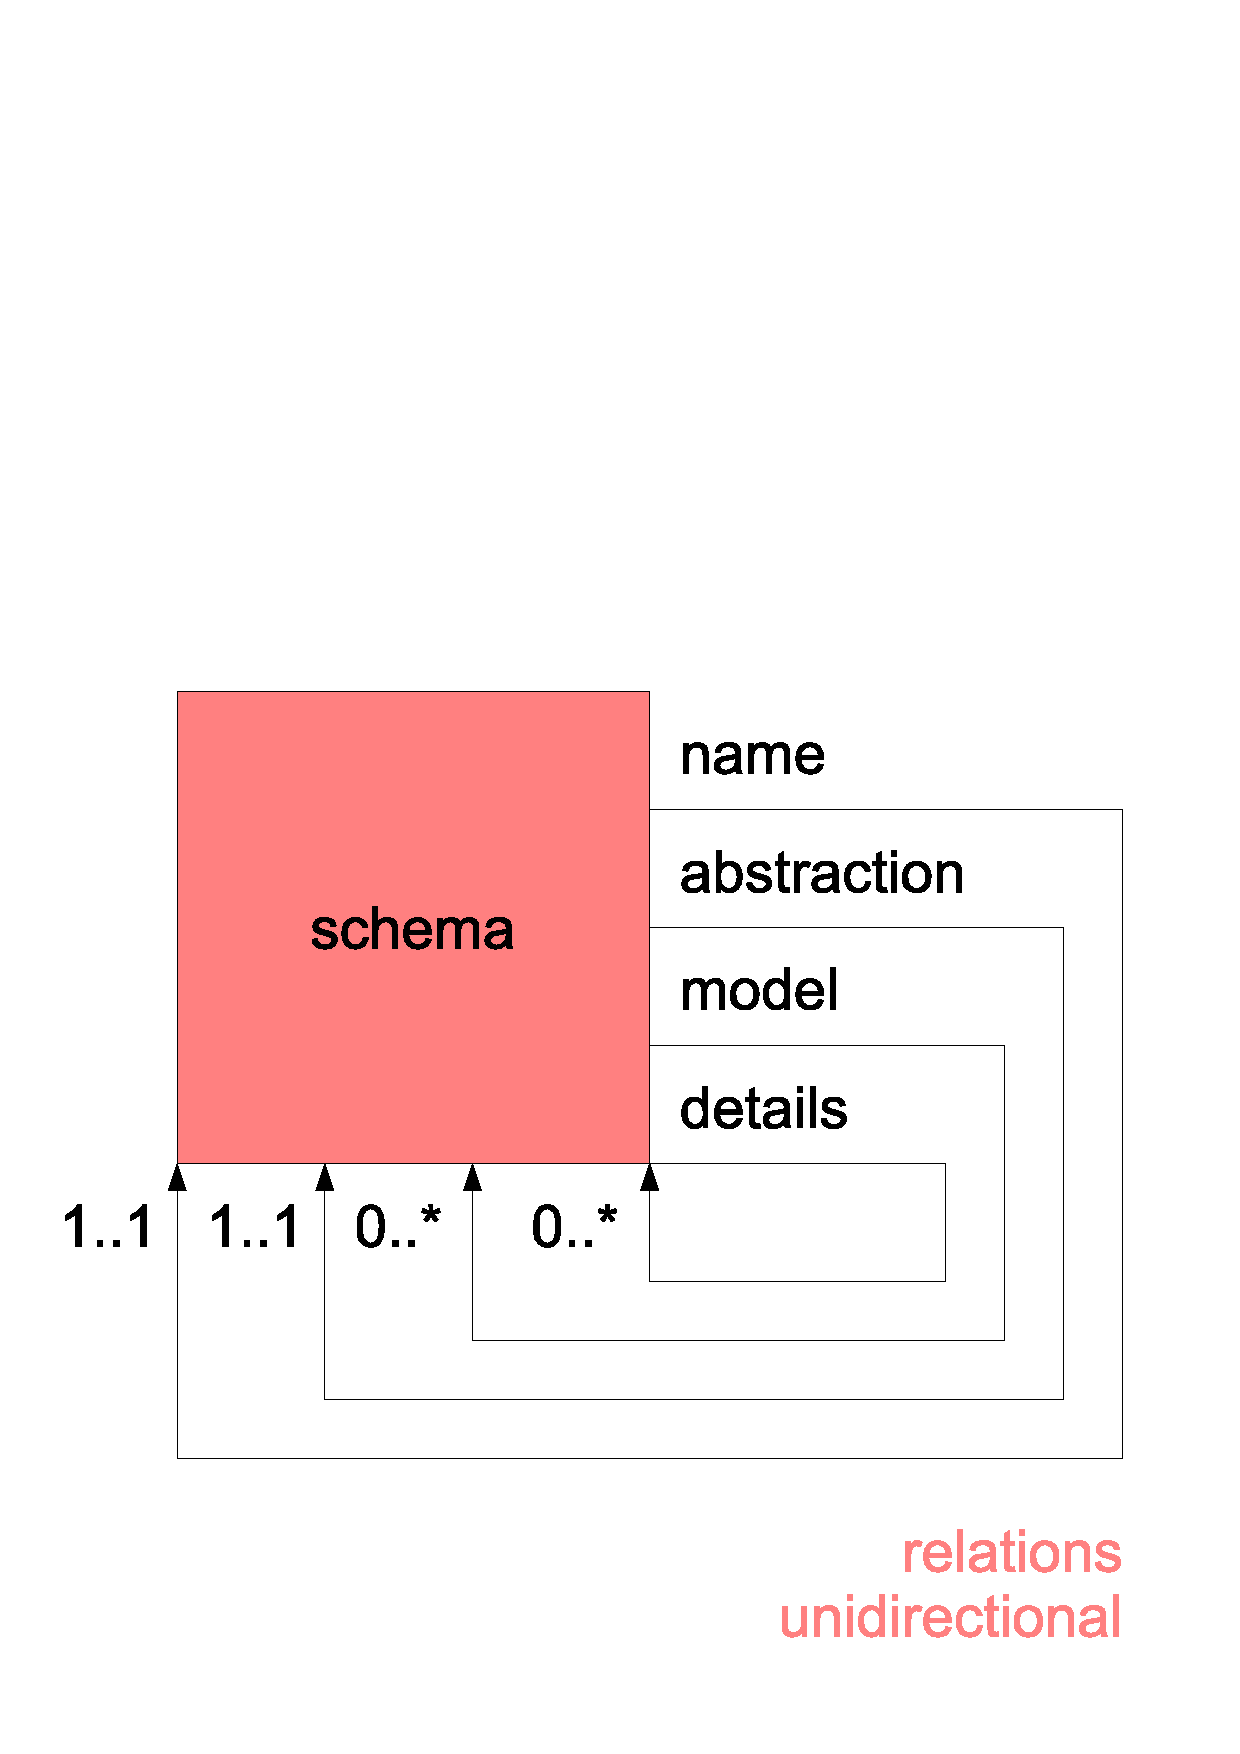
\includegraphics[scale=0.3,angle=-90]{graphic/schema.pdf}
        \caption{Knowledge Schema with Meta Information about Parts}
        \label{schema_figure}
    \end{center}
\end{figure}

Yet what does this knowledge of a compound model (whole) about its parts imply?
Software developers call knowledge \emph{about} something \emph{Meta Information}.
Figure \ref{schema_figure} shows the four essential kinds of meta information in
a whole-part relation. Software developers might want to call the illustration
of these relations a \emph{Schema} or \emph{Meta Model}.

An obvious way is to give each part a unique \emph{Name} for identification.
The concept of a human body, for example, would have parts like heart, brain,
left\_arm and so on.

Secondly, a compound needs to know about the \emph{Model} of each part since a
part may itself be seen as compound that needs to know about its parts. Although
all real world items can be modelled as compound, it does not make sense to do
so in the virtual world of the human mind. As mentioned before, models have to
be limited in their information contents, towards microcosm as well as towards
macrocosm, in order to be comprehensible by the human mind. It is therefore
necessary to introduce primitive models like a word or a number (compare
\emph{Quality and Quantity}, section \ref{quality_and_quantity_heading}),
representing the final form of abstraction in a compound.

The distinction of the several kinds of models, in other words the kind of
\emph{Abstraction} (compound, term, number etc.) of a model is the third
kind of information a compound needs to know about its parts. It is comparable
to a \emph{Type} in classical system programming languages (section
\ref{system_programming_heading}).

All further kinds of meta information are summed up by a fourth relation which
is called \emph{Details} in this work. Just like the \emph{Model}, it is a
dynamically extensible structure. It will be explained in the following section.

The suggested knowledge model uses a simple \emph{Tree} structure, capable of
referencing parts of arbitrary type. It does not follow the \emph{Composite}
software pattern (section \ref{composite_heading}), because the meta information
whether a part model is a compound (composite) or not (leaf) does not belong
into the model structure. Section \ref{categorisation_versus_composition_heading}
explained this design mistake on the example of \emph{Party} types. It is not
good to fix some model as leave, at design time. Who knows if at runtime
(during program execution), that model would not have to have any parts?
As an aside: A similar design (simple tree structure) is used by the
\emph{Java Swing} framework \cite{java}, for example. Its tree node class
\emph{DefaultMutableTreeNode} represents a \emph{Tree Node} and
\emph{Tree Container}, at the same time.

%
% $RCSfile: double_hierarchy.tex,v $
%
% Copyright (C) 2002-2008. Christian Heller.
%
% Permission is granted to copy, distribute and/or modify this document
% under the terms of the GNU Free Documentation License, Version 1.1 or
% any later version published by the Free Software Foundation; with no
% Invariant Sections, with no Front-Cover Texts and with no Back-Cover
% Texts. A copy of the license is included in the section entitled
% "GNU Free Documentation License".
%
% http://www.cybop.net
% - Cybernetics Oriented Programming -
%
% http://www.resmedicinae.org
% - Information in Medicine -
%
% Version: $Revision: 1.1 $ $Date: 2008-08-19 20:41:06 $ $Author: christian $
% Authors: Christian Heller <christian.heller@tuxtax.de>
%

\subsection{Double Hierarchy}
\label{double_hierarchy_heading}
\index{Double Hierarchy}
\index{Whole-Part Relationship}
\index{Dialectical Relationship between Whole and Part}
\index{Conceptual Interaction}
\index{Part}
\index{Property}
\index{Constraint}

Finally, what makes up the character of a model (in the understanding of the
human mind) is a combination of two hierarchies: the \emph{Parts} it consists
of, together with \emph{Meta Information} about it.

Most properties of a molecule in \emph{Chemistry}, for example, are determined
by the number and arrangement of its atoms. \emph{Hydrogen} (H$_{2}$) becomes
\emph{Water} (H$_{2}$O) (with a totally different character) when just one
\emph{Oxygen} (O) atom is added per hydrogen molecule. The Wikipedia Encyclopedia
\cite{wikipedia} cites and writes about Richard Levins and Richard Lewontin
who, in their book \textit{The Dialectical Biologist} \cite{levins}, sketch a
\emph{dialectical} approach to biology:

\begin{quote}
    They focus on the (dialectical) relationship between the \emph{Whole} (or
    \emph{Totality}) and the \emph{Parts}: \textit{Part makes Whole, and Whole
    makes Part} \cite[p. 272]{levins}. That is, a biological system of some kind
    consists of a collection of heterogeneous parts. All of these contribute to
    the character of the whole, as in reductionist thinking. On the other hand,
    the whole has an existence independent of the parts and feeds back to affect
    and determine the nature of the parts. This back-and-forth (dialectic) of
    causation implies a dynamic process. \ldots\ Further, each species is part
    of the \emph{Environment} of all of the others.
\end{quote}

The kinds of meta information discussed in the previous sections were also
called \emph{Dimensions} or \emph{Conceptual Interaction} between a \emph{Whole}
and its \emph{Parts}. They may represent very different properties and each of
them may be constrained to certain values- or areas of validity.

\begin{figure}[ht]
    \begin{center}
        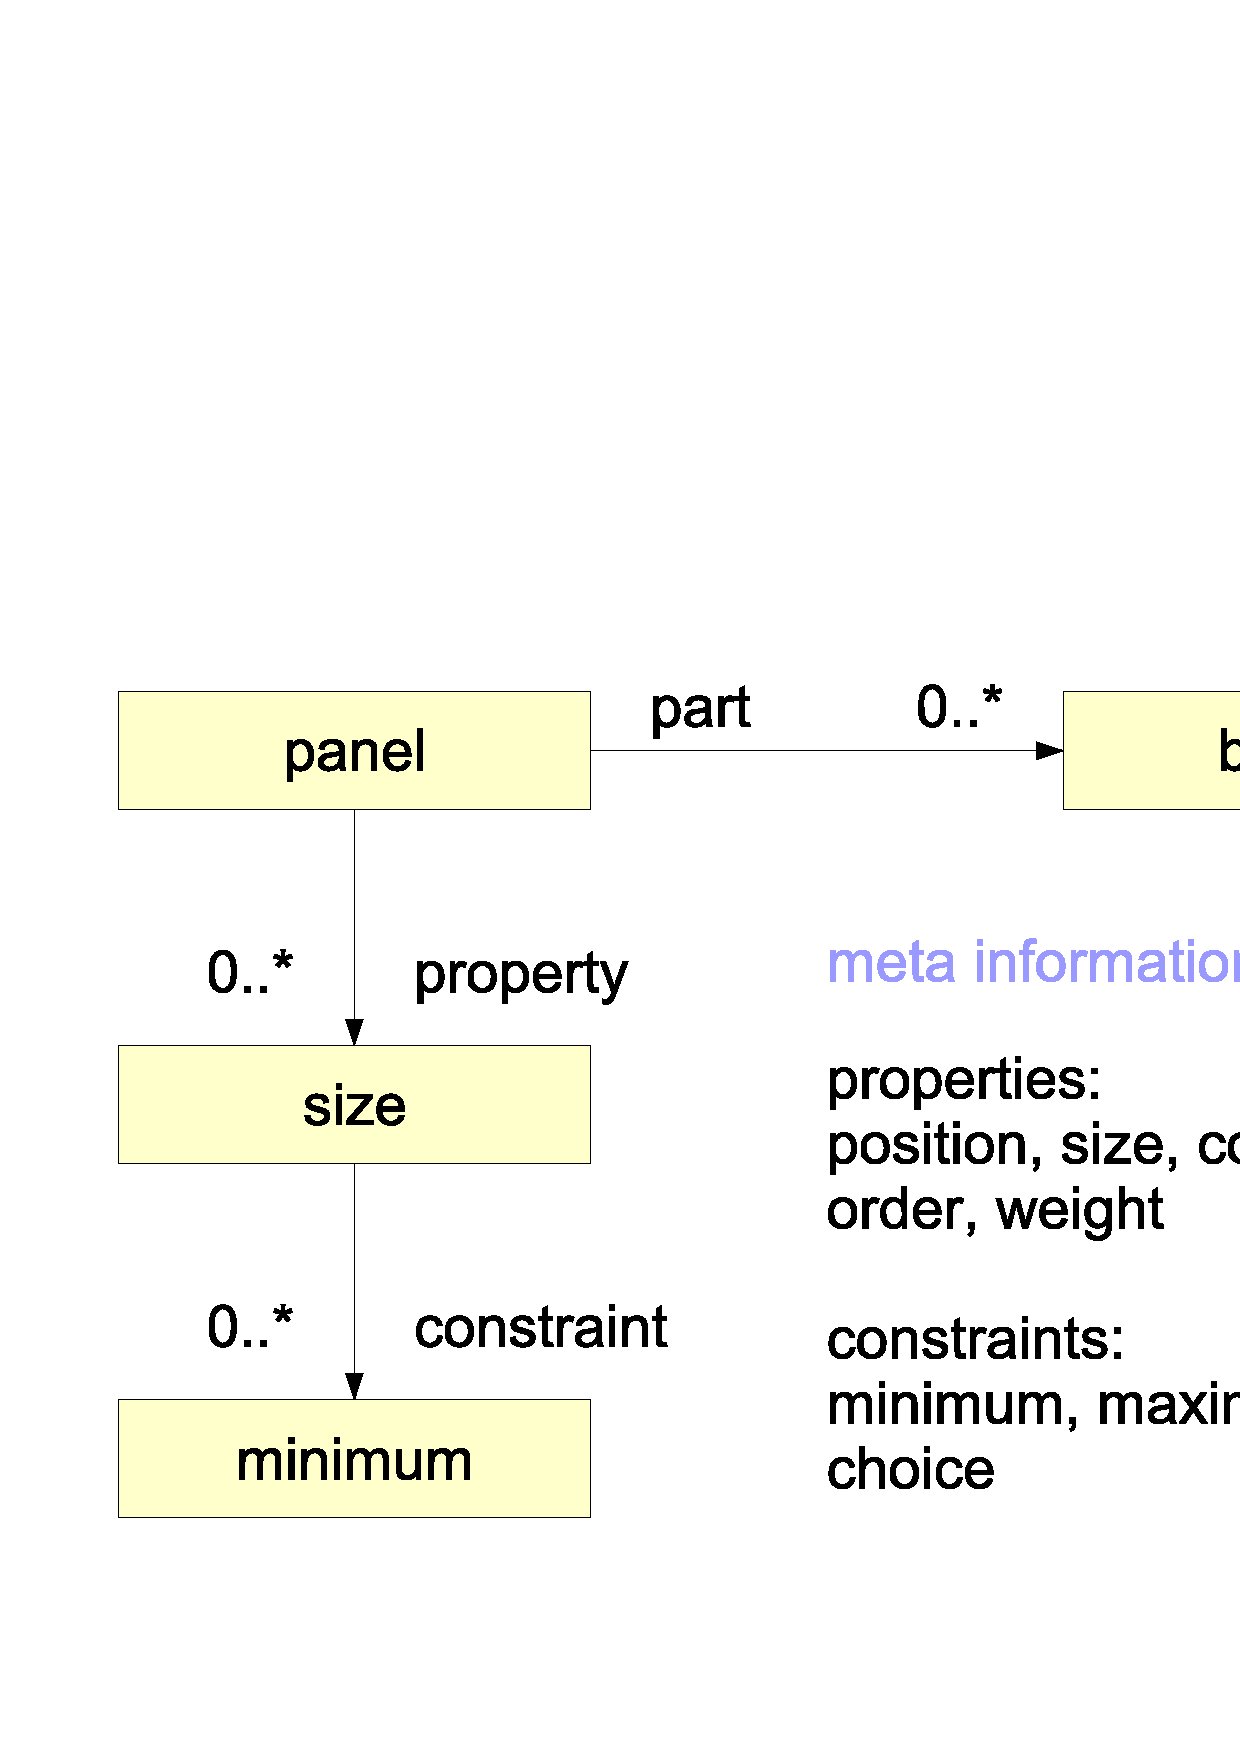
\includegraphics[scale=0.3,angle=-90]{graphic/double.pdf}
        \caption{Double Hierarchy of Parts and Meta Information}
        \label{double_figure}
    \end{center}
\end{figure}

Figure \ref{double_figure} illustrates the \emph{Double Hierarchy} here
spoken of. A graphical panel was chosen as example model. It may consist of
smaller parts, among them being a number of buttons. Altogether, they form the
\emph{Part Hierarchy}. On the other hand, there are properties like the size,
position or colour of the buttons, which are neither part of the panel, nor of
the buttons themselves; they are information \emph{about} the buttons and form
an own \emph{Meta Hierarchy}. To the latter do also belong constraints like the
minimum size of a button or a possible choice of colours for it. Constraints can
be treated like meta information about properties. Once again: \emph{Properties}
are information about a \emph{Part}; \emph{Constraints} are information about a
\emph{Property}.

%
% $RCSfile: container_unification.tex,v $
%
% Copyright (C) 2002-2008. Christian Heller.
%
% Permission is granted to copy, distribute and/or modify this document
% under the terms of the GNU Free Documentation License, Version 1.1 or
% any later version published by the Free Software Foundation; with no
% Invariant Sections, with no Front-Cover Texts and with no Back-Cover
% Texts. A copy of the license is included in the section entitled
% "GNU Free Documentation License".
%
% http://www.cybop.net
% - Cybernetics Oriented Programming -
%
% http://www.resmedicinae.org
% - Information in Medicine -
%
% Version: $Revision: 1.1 $ $Date: 2008-08-19 20:41:06 $ $Author: christian $
% Authors: Christian Heller <christian.heller@tuxtax.de>
%

\subsection{Container Unification}
\label{container_unification_heading}
\index{Container Unification}
\index{Container}
\index{Collection as Container}
\index{Array as Container}
\index{Vector as Container}
\index{Stack as Container}
\index{Set as Container}
\index{List as Container}
\index{Map as Container}
\index{Hash Map as Container}
\index{Hash Table as Container}
\index{Tree as Container}

Section \ref{falsifying_polymorphism_heading} demonstrated how container
inheritance, due to polymorphism, may cause unpredictable behaviour leading to
\emph{falsified} container contents. The sections of this chapter introduced a
knowledge schema which they claimed to be \emph{general}. But that also means
that all kinds of containers must be representable by the suggested schema. But
why are there so many different kinds of containers? What actually is a
container?

It is a concept expressing that some model \emph{contains} some other model(s).
Types of containers that were introduced in section \ref{container_heading} are
\emph{Collections} (Array, Vector, Stack, Set, List), \emph{Maps} (Hash Map,
Hash Table) and the \emph{Tree}. They all are containers. What differs is just
the meta information they store about their elements. A list, for example,
holds position information about each of its elements. A map relates the name
of an element to its model (1:1). A tree links one model to many others (1:n).

But does the different meta information a container holds about its elements
justify the existence of different container models? If a knowledge schema was
general enough to represent a container structure on one hand, and to express
different kinds of meta information on the other, it might be able to behave
like \emph{any} of the known container types.

The schema proposed in this work claims to be this kind of knowledge schema. It
has a container structure by default, and can thus hold many parts in a
\emph{Tree}-like manner. It holds standard meta information about its parts:
their \emph{Name}, \emph{Model}, kind of \emph{Abstraction} and further meta
information called \emph{Details} -- and is therefore able to link the name of
an element to its model, in a \emph{Map}-like manner. To the additional meta
information (details) may belong the \emph{Position} of an element within its
model, in a \emph{List}-like manner. A \emph{Table} structure can be represented
as well, by splitting it into a hierarchical (tree-like) representation, as
known from markup languages (section \ref{markup_language_heading}).

Chapter \ref{cybernetics_oriented_language_heading} will introduce a language
capable of expressing all aspects of the knowledge schema as proposed in this
chapter.

%
% $RCSfile$
%
% Copyright (c) 2002-2006. Christian Heller. All rights reserved.
%
% Permission is granted to copy, distribute and/or modify this document
% under the terms of the GNU Free Documentation License, Version 1.1 or
% any later version published by the Free Software Foundation; with no
% Invariant Sections, with no Front-Cover Texts and with no Back-Cover
% Texts. A copy of the license is included in the section entitled
% "GNU Free Documentation License".
%
% http://www.cybop.net
% - Cybernetics Oriented Programming -
%
% http://www.resmedicinae.org
% - Information in Medicine -
%
% Version: $Revision$ $Date$ $Author$
% Authors: Christian Heller <christian.heller@tuxtax.de>
%

\subsubsection{Universal Memory Structure}
\label{universal_memory_structure_heading}

To better explain the differences between traditional- and cybernetics-oriented
design models, an example shall help. (A first one was given in section
\ref{modelling_mistakes_heading}, which showed modelling mistakes at the
concept of a horse.) Figure \ref{universal_figure} illustrates design-time
structures in the upper half, and runtime structures in the lower. Using
\emph{Structured- and Procedural Programming} (SPP) or
\emph{Object Oriented Programming} (OOP), a developer would design a model as
shown on the upper left-hand side in the figure. (The fact that OOP also offers
inheritance relations and OOP classes do own methods in addition to attributes,
while SPP structures do not, is of minor importance here.) At runtime, exactly
that model would be applied to structure instances and their relations
accordingly, as shown on the lower left-hand side in the figure.

\begin{figure}[ht]
    \begin{center}
        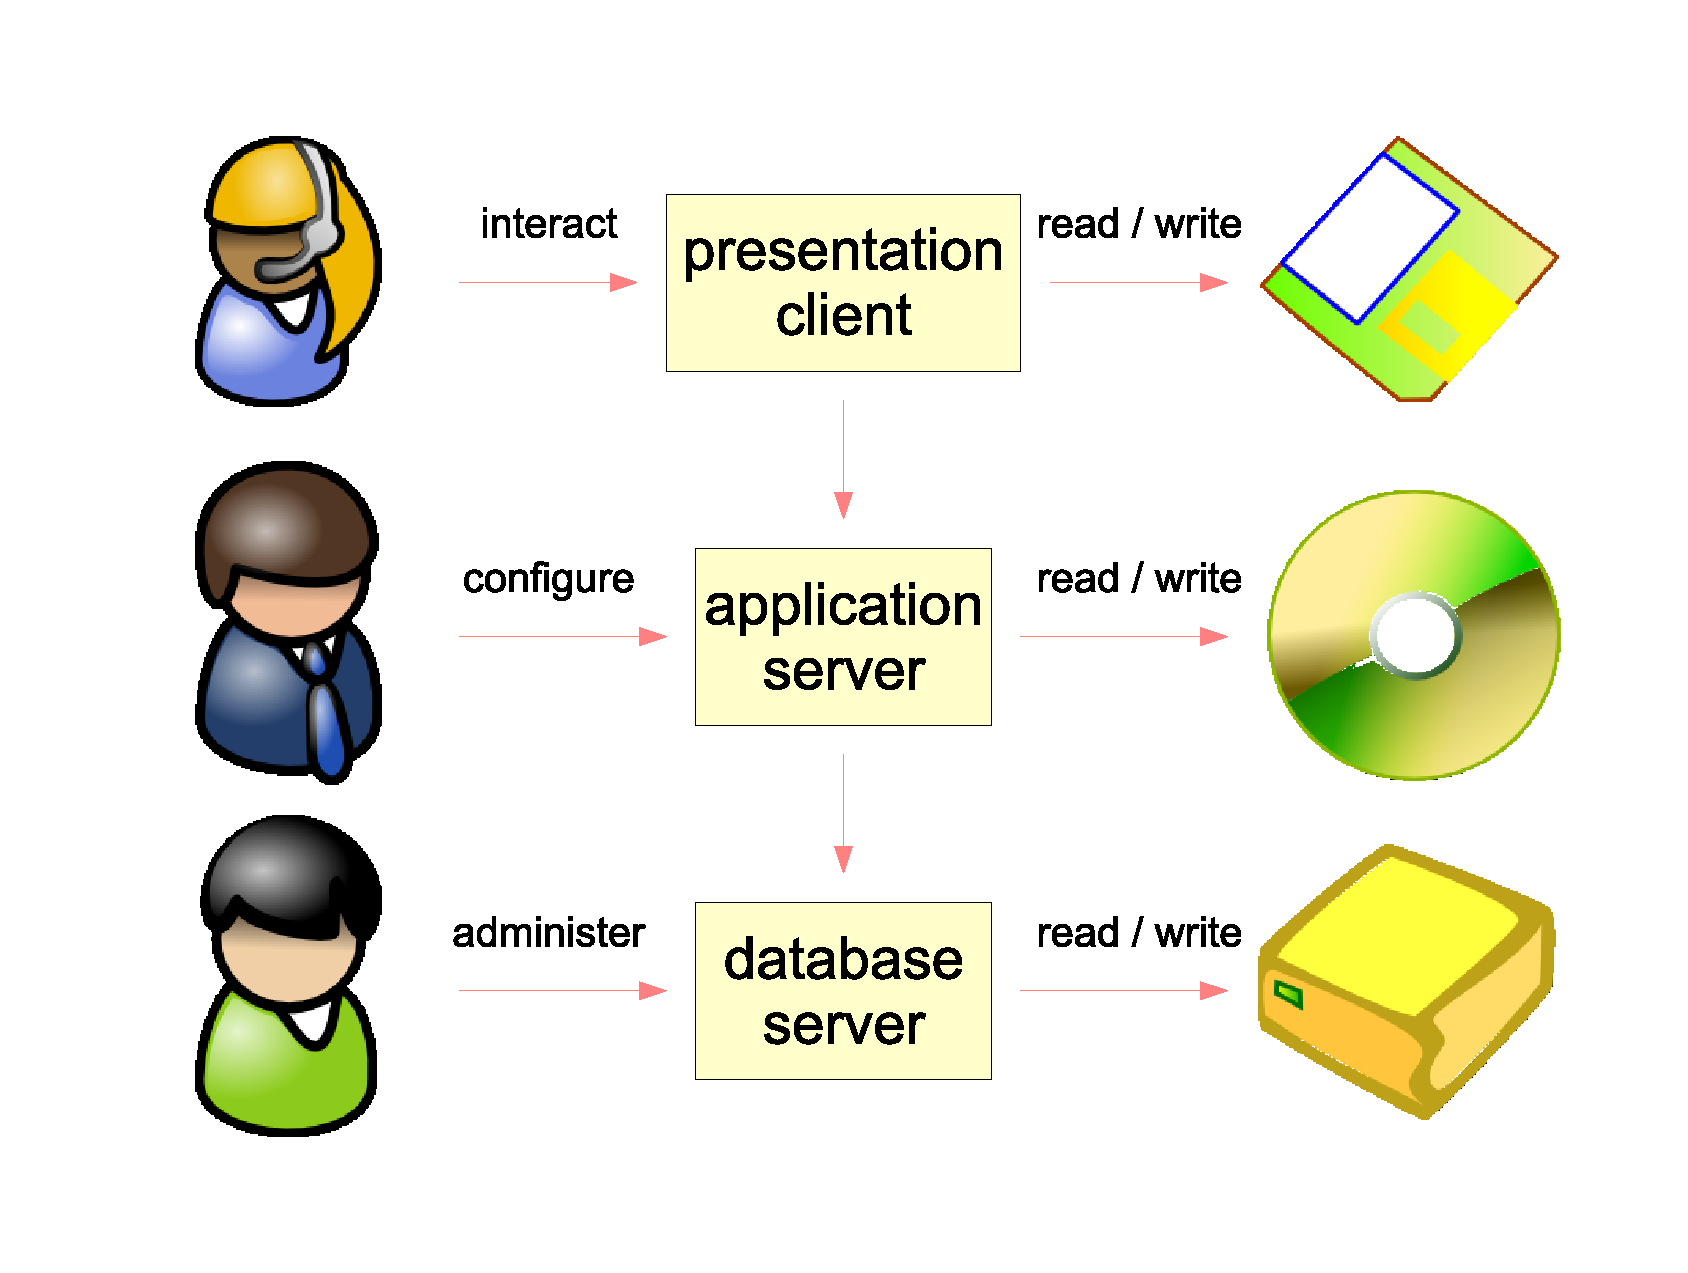
\includegraphics[scale=0.2]{vector/universal.eps}
        \caption{Universal Memory Structure}
        \label{universal_figure}
    \end{center}
\end{figure}

Not so in \emph{Cybernetics Oriented Programming} (CYBOP). Knowledge templates
as created at design time do always have a hierarchical structure, as shown on
the upper right-hand side in the figure. They include \emph{Whole-Part-} as
well as \emph{Meta Hierarchies} (the latter neglected in the figure). At
runtime, these templates get cloned by creating models that follow the
structure of the CYBOP \emph{Knowledge Schema}, as shown on the lower
right-hand side in the figure. While SPP/ OOP rely on a variety of different
structures to store knowledge in memory, CYBOP uses one
\emph{Universal Memory Structure} (knowledge schema) that, so to say, merges
traditional structures like different kinds of \emph{Containers}, \emph{Class}
and \emph{Record}/\emph{Struct}. Even algorithmic structures (logic)
traditionally stored in a \emph{Procedure} are covered by this knowledge
schema. More on state and logic in the following section.

The advantages are obvious. Data available in a unified structure are easier to
process. Dependencies of the knowledge schema are defined clearly and remain
the same for all applications, so that domain/ application knowledge becomes
independent from the underlying system control software. Global data access and
bidirectional dependencies are not necessary anymore, since every knowledge
model can be accessed along well-defined paths within the knowledge hierarchy.
Byte code manipulation and similar tricks and workarounds might finally belong
to the past.


%
% $RCSfile: state_and_logic.tex,v $
%
% Copyright (c) 2005-2006. Christian Heller. All rights reserved.
%
% Permission is granted to copy, distribute and/or modify this document
% under the terms of the GNU Free Documentation License, Version 1.1 or
% any later version published by the Free Software Foundation; with no
% Invariant Sections, with no Front-Cover Texts and with no Back-Cover
% Texts. A copy of the license is included in the section entitled
% "GNU Free Documentation License".
%
% http://www.cybop.net
% - Cybernetics Oriented Programming -
%
% http://www.resmedicinae.org
% - Information in Medicine -
%
% Version: $Revision: 1.1 $ $Date: 2006-01-03 08:21:45 $ $Author: christian $
% Authors: Christian Heller <christian.heller@tuxtax.de>
%

\subsection{State and Logic}
\label{state_and_logic_heading}

According to the observations made in the work described in this article, there
are two kinds of knowledge: \emph{State-} and \emph{Logic}. While the former
may be placed in a spatial dimension, the latter is processed as sequence over
time. Often, logic is labelled \emph{dynamic} behaviour -- but only the
\emph{execution} of a rule of logic is dynamic, \emph{not} the rule itself
(\emph{static}).

Rules of logic translate input- into output states. What
characterises a system is how it applies logic knowledge to translate state
knowledge \cite{heller2002}. Yet how to imagine a knowledge model consisting of
state- as well as logic parts? Following an example.

The famous \emph{Model View Controller} (MVC) pattern was extended by the
\emph{Hierarchical MVC} (HMVC) pattern towards a hierarchy of \emph{MVC Triads}
\cite{cai}. The omnipresence of hierarchies in the MVC was demonstrated in
\cite{hellerbohl}.

\begin{figure}[ht]
    \begin{center}
        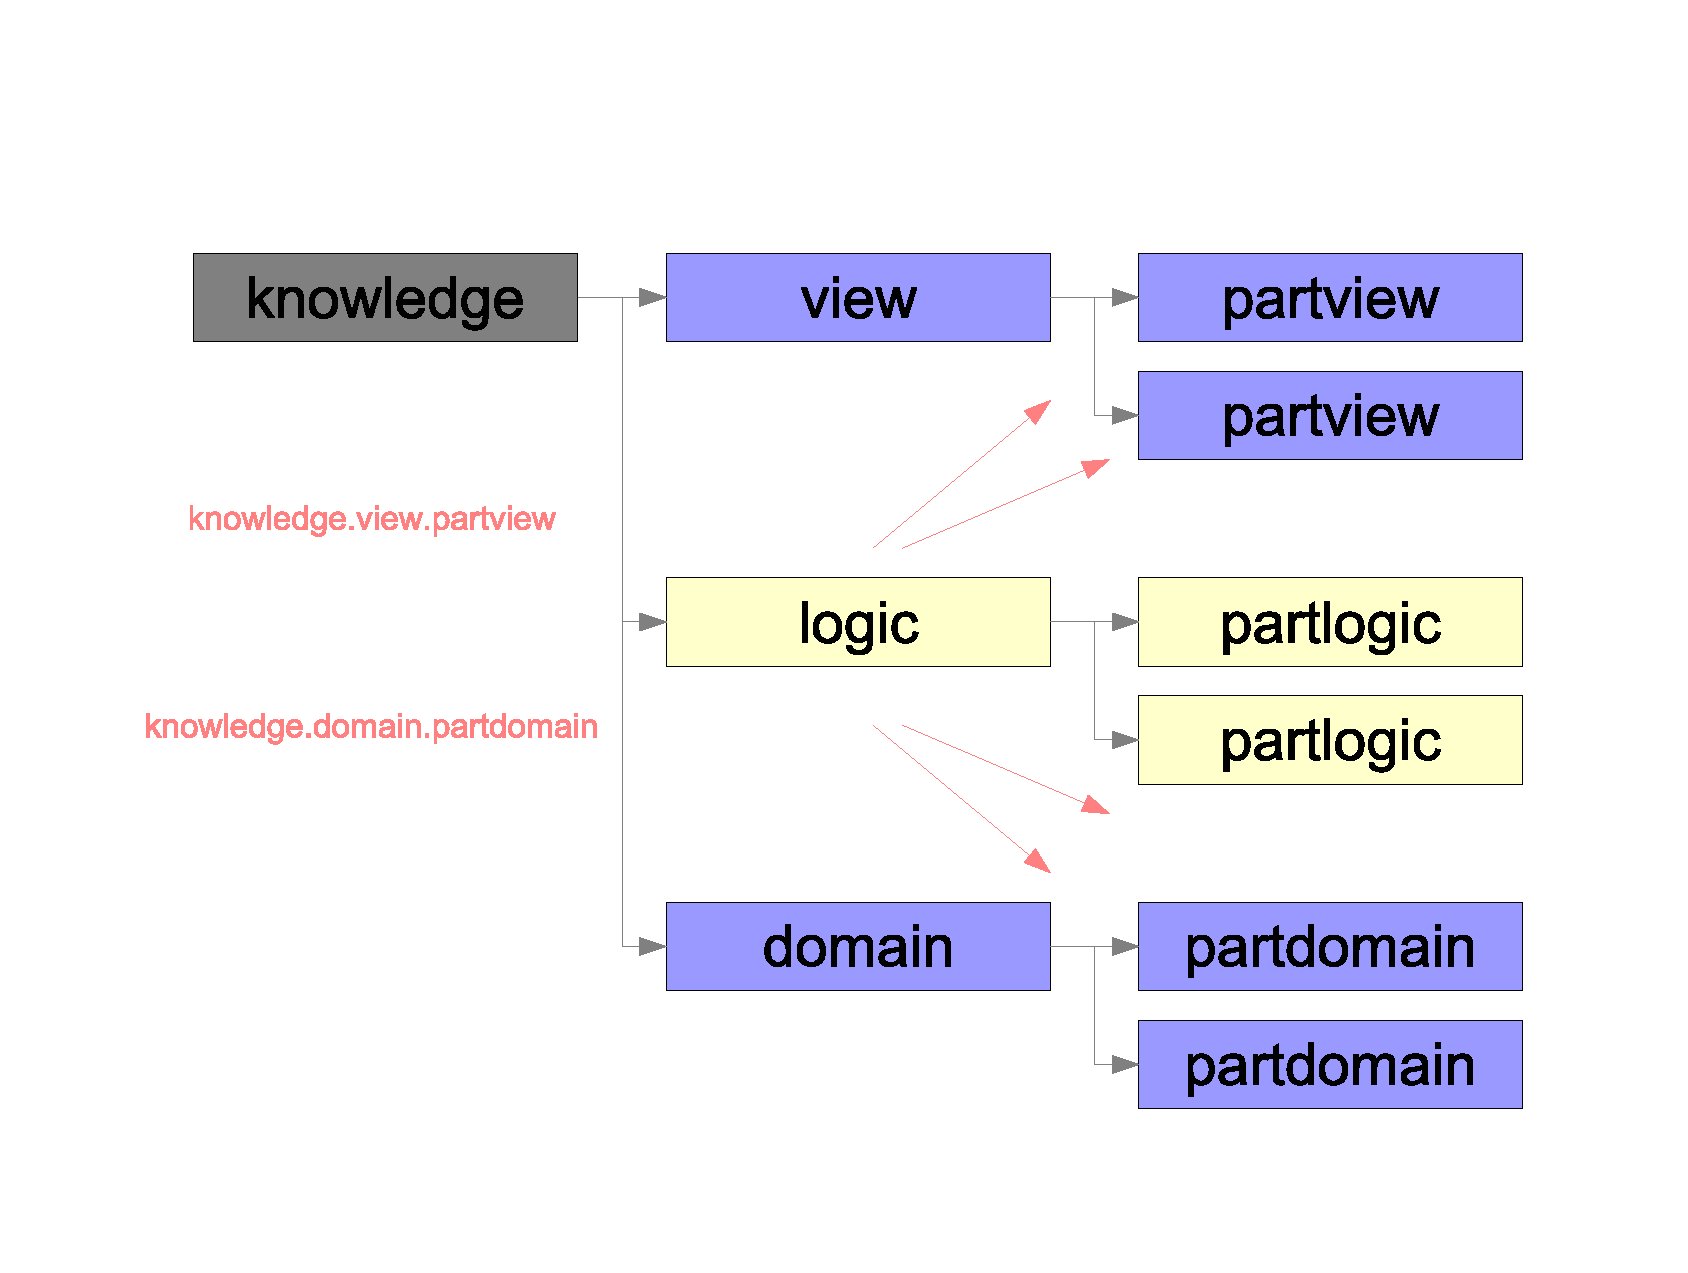
\includegraphics[scale=0.2]{vector/mvctree.eps}
        \caption{Runtime Logic manipulating States}
        \label{mvctree_figure}
    \end{center}
\end{figure}

Figure \ref{mvctree_figure} shows the three parts: \emph{Domain} (Model),
\emph{View} and \emph{Logic} (Controller) of an (adapted) MVC pattern as
independent branches of one common knowledge tree, as existent at system
runtime in memory. Each of them represents a concept on its own. The logic
model, however, is allowed to access and change the view- and domain model; it
is able to link different knowledge models. But view- and domain model,
representing states, are not allowed to manipulate logic. In other words: The
dependencies between logic- and state models are \emph{unidirectional}.

An innovation is that logic knowledge gets manipulatable. A logic model
(algorithm) cannot only access and change state-, but also logic models, even
itself! Because models modified in that manner can be made persistent in form
of CYBOL knowledge templates (section \ref{practical_proof_heading}), and be
reloaded the next time an application starts, this may be seen as a kind of
\emph{Meta Programming} \cite{wikipedia}.

The clear separation of states and logic into discrete models avoids unwanted
dependencies as caused by the bundling of attributes and methods in OOP. All
that would be needed to make a CYBOP system work with new state models, is the
corresponding translation logic. Translators \cite{hellerkunze} simplify
architectures and unify communication.


    %
% $RCSfile$
%
% Copyright (c) 2005-2006. Christian Heller. All rights reserved.
%
% Permission is granted to copy, distribute and/or modify this document
% under the terms of the GNU Free Documentation License, Version 1.1 or
% any later version published by the Free Software Foundation; with no
% Invariant Sections, with no Front-Cover Texts and with no Back-Cover
% Texts. A copy of the license is included in the section entitled
% "GNU Free Documentation License".
%
% http://www.cybop.net
% - Cybernetics Oriented Programming -
%
% http://www.resmedicinae.org
% - Information in Medicine -
%
% Version: $Revision$ $Date$ $Author$
% Authors: Christian Heller <christian.heller@tuxtax.de>
%

\section{Practical Proof}
\label{practical_proof_heading}

The proof of operatability for the new concepts is given by the
\emph{Cybernetics Oriented Language} (CYBOL), defined according to the
principles of abstraction worked out before, and by the
\emph{Cybernetics Oriented Interpreter} (CYBOI), a knowledge processing system.
In addition, a prototype application called \emph{Res Medicinae}
\cite{resmedicinae} was implemented in CYBOL.

%
% $RCSfile: cybol.tex,v $
%
% Copyright (c) 2002-2007. Christian Heller. All rights reserved.
%
% Permission is granted to copy, distribute and/or modify this document
% under the terms of the GNU Free Documentation License, Version 1.1 or
% any later version published by the Free Software Foundation; with no
% Invariant Sections, with no Front-Cover Texts and with no Back-Cover
% Texts. A copy of the license is included in the section entitled
% "GNU Free Documentation License".
%
% http://www.cybop.net
% - Cybernetics Oriented Programming -
%
% Version: $Revision: 1.1 $ $Date: 2007-07-17 20:02:36 $ $Author: christian $
% Authors: Christian Heller <christian.heller@tuxtax.de>
%

%
% Determine document class specifying the type of document.
%
% Hand over font size and side format.
%
%\documentclass[9pt,twoside]{tuxtax}
\documentclass[10pt,twoside]{tuxtax}

%
% Input hyphenation list.
%
%%
% $RCSfile: hyphenation.tex,v $
%
% Copyright (c) 2001-2004. Christian Heller. All rights reserved.
%
% No copying, altering, distribution or any other actions concerning this
% document, except after explicit permission by the author!
% At some later point in time, this document is planned to be put under
% the GNU FDL license. For now, _everything_ is _restricted_ by the author.
%
% http://www.cybop.net
% - Cybernetics Oriented Programming -
%
% http://www.resmedicinae.org
% - Information in Medicine -
%
% @author Christian Heller <christian.heller@tuxtax.de>
%

\hyphenation{abs-trac-tion}
\hyphenation{abs-trac-tions}
\hyphenation{ac-tu-ally}
\hyphenation{addi-tio-nally}
\hyphenation{ana-lyst}
\hyphenation{ana-ly-sis}
\hyphenation{an-cient}
\hyphenation{ap-pli-ca-tion}
\hyphenation{arche-types}
\hyphenation{aris-to-tle}
\hyphenation{at-tri-bute}
\hyphenation{avoi-da-ble}
\hyphenation{be-ing}
\hyphenation{binary}
\hyphenation{bran-ches}
\hyphenation{ca-te-go-ri-za-tion}
\hyphenation{client}
\hyphenation{com-po-nen-ti-za-tion}
\hyphenation{com-pu-ter}
\hyphenation{con-fi-gure}
\hyphenation{con-fi-gu-ra-tion}
\hyphenation{con-nec-ted}
\hyphenation{cri-ti-cised}
\hyphenation{cy-ber-ne-tics}
\hyphenation{cyboi}
\hyphenation{cybol}
\hyphenation{cybop}
\hyphenation{de-sign}
\hyphenation{des-cribe}
\hyphenation{des-cribed}
\hyphenation{de-ve-lop-ment}
\hyphenation{dis-crete}
\hyphenation{di-vide}
\hyphenation{do-main}
\hyphenation{dy-na-mic}
\hyphenation{dy-na-mics}
\hyphenation{ela-bo-ra-ted}
\hyphenation{ele-ments}
\hyphenation{en-gi-nee-ring}
\hyphenation{eng-lish}
\hyphenation{en-vi-ron-ment}
\hyphenation{ex-pert}
\hyphenation{fi-gure}
\hyphenation{fun-da-men-tal}
\hyphenation{func-tio-na-li-ty}
\hyphenation{hard-ware}
\hyphenation{hu-man}
\hyphenation{im-ple-men-ta-tion}
\hyphenation{imp-roved}
\hyphenation{in-he-rit}
\hyphenation{in-ter-pre-ter}
\hyphenation{java}
\hyphenation{know-ledge}
\hyphenation{lan-guage}
\hyphenation{li-ving}
\hyphenation{lo-gi-cal}
\hyphenation{machine}
\hyphenation{me-cha-nism}
\hyphenation{me-thods}
\hyphenation{na-ture}
\hyphenation{net-work}
\hyphenation{neu-ral}
\hyphenation{neu-ron}
\hyphenation{nu-me-rous}
\hyphenation{object}
\hyphenation{open}
\hyphenation{operating}
\hyphenation{ori-en-ted}
\hyphenation{over-come}
\hyphenation{prin-ci-ple}
\hyphenation{prin-ting}
\hyphenation{pro-ba-bi-lis-tic}
\hyphenation{pro-gram-ming}
\hyphenation{re-cog-nize}
\hyphenation{re-cog-nized}
\hyphenation{re-pre-sen-ta-tion}
\hyphenation{re-pre-sen-ting}
\hyphenation{re-u-sa-bi-li-ty}
\hyphenation{sci-ence}
\hyphenation{server}
\hyphenation{se-pa-ra-ted}
\hyphenation{se-pa-ra-tion}
\hyphenation{si-mi-lar}
\hyphenation{soft-ware}
\hyphenation{source}
\hyphenation{spe-cia-li-za-tion}
\hyphenation{sta-tic}
\hyphenation{sta-ti-cal-ly}
\hyphenation{sto-chas-tic}
\hyphenation{stone-on-stone}
\hyphenation{struc-ture}
\hyphenation{strug-gling}
\hyphenation{su-per-flu-ous}
\hyphenation{sup-ply-ing}
\hyphenation{sys-tem}
\hyphenation{tes-ting}
\hyphenation{thin-king}
\hyphenation{un-en-li-vened}
\hyphenation{un-fa-vou-ra-ble}
\hyphenation{un-sa-tis-fy-ing}
\hyphenation{va-ry-ing}
\hyphenation{weigh-ted}


%
% Define text macros.
%
\def\placemacro{Ilmenau}
\def\datemacro{2007-07-06}
\def\authormacro{Christian Heller}

%
% Enable special indexing commands.
% Generate contents, glossary and memo entries.
%
% Required package: makeidx
%
\makeindex

%
% This document describes the Cybernetics Oriented Language (CYBOL).
%
% Author: Christian Heller <christian.heller@tuxtax.de>
%
\begin{document}
    % Set sans serif font.
    \sffamily
    % Set page numbering to roman numbers.
    \pagenumbering{roman}
    %
% $RCSfile: cover.tex,v $
%
% Copyright (C) 2002-2008. Christian Heller.
%
% Permission is granted to copy, distribute and/or modify this document
% under the terms of the GNU Free Documentation License, Version 1.1 or
% any later version published by the Free Software Foundation; with no
% Invariant Sections, with no Front-Cover Texts and with no Back-Cover
% Texts. A copy of the license is included in the section entitled
% "GNU Free Documentation License".
%
% http://www.cybop.net
% - Cybernetics Oriented Programming -
%
% http://www.resmedicinae.org
% - Information in Medicine -
%
% Version: $Revision: 1.1 $ $Date: 2008-08-19 20:41:06 $ $Author: christian $
% Authors: Christian Heller <christian.heller@tuxtax.de>
%

%
% Defines the title page.
%
% \title and \author (and optionally \date) must be specified!
%
% Sets the page style of the first page to empty
% that is no header or footer will be shown.
%
\begin{titlepage}
    \title{
        Cybernetics Oriented Programming\\
        (CYBOP)\\
        \vspace{1cm}
        % \textmd sets medium weight (default), which is the opposite of boldface.
        \normalsize{\textmd{An Investigation on the Applicability of Inter-Disciplinary Concepts\\
            to Software System Development\\}}
    }
    \author{
        \date{
        }
    }
\end{titlepage}

    \maketitle
    % Avoid header, footer and page number.
    \thispagestyle{empty}
    %
% $RCSfile: title.tex,v $
%
% Copyright (c) 2001-2004. Christian Heller. All rights reserved.
%
% No copying, altering, distribution or any other actions concerning this
% document, except after explicit permission by the author!
% At some later point in time, this document is planned to be put under
% the GNU FDL license. For now, _everything_ is _restricted_ by the author.
%
% http://www.cybop.net
% - Cybernetics Oriented Programming -
%
% http://www.resmedicinae.org
% - Information in Medicine -
%
% @author Christian Heller <christian.heller@tuxtax.de>
%

\title{A new Pattern Systematics}
\author{
    Christian Heller \(<\)christian.heller@tu-ilmenau.de\(>\)\\
    Detlef Streitferdt \(<\)detlef.streitferdt@tu-ilmenau.de\(>\)\\
    Ilka Philippow \(<\)ilka.philippow@tu-ilmenau.de\(>\)
}
\institute{Technical University of Ilmenau\\
    Faculty for Computer Science and Automation\\
    Institute for Theoretical and Technical Informatics\\
    PF 100565, Max-Planck-Ring 14, 98693 Ilmenau, Germany\\
    http://www.tu-ilmenau.de, fon: +49-3677-69-1230, fax: +49-3677-69-1220 \vspace*{0.5cm}
}

    \newpage{\pagestyle{empty}\clearpage}
    \thispagestyle{empty}
    %
% $RCSfile: copyright.tex,v $
%
% Copyright (c) 2002-2007. Christian Heller. All rights reserved.
%
% Permission is granted to copy, distribute and/or modify this document
% under the terms of the GNU Free Documentation License, Version 1.1 or
% any later version published by the Free Software Foundation; with no
% Invariant Sections, with no Front-Cover Texts and with no Back-Cover
% Texts. A copy of the license is included in the section entitled
% "GNU Free Documentation License".
%
% http://www.cybop.net
% - Cybernetics Oriented Programming -
%
% Version: $Revision: 1.2 $ $Date: 2007-08-01 13:59:00 $ $Author: christian $
% Authors: Christian Heller <christian.heller@tuxtax.de>
%

\small{Cataloging-in-Publication Data\\\\
    \authormacro.\\
    \titlemacro:\\
    \subtitlemacro\\
    \versionmacro\\
    \placemacro: Tux Tax, 2007%\\
%    ISBN-10: 3-9810898-0-4 xxx EDIT xxx\\
%    ISBN-13: 978-3-9810898-0-6 xxx EDIT xxx
}\\

\small{Information about this specification\\
    http://www.cybop.net, http://www.tuxtax.de}

\vspace{4cm}

\small{Copyright \textcopyright\ 2002-2007. \authormacro. All rights reserved.}

%> \small{Translation: Christian Heller}\\ %\"Ubersetzung:
%\small{Sponsoring Editor: ??}\\ %Lektorat:
%\small{Acquisitions Editor: ??}\\
%\small{Marketing Manager: ??}\\
%\small{Marketing Assistant: ??}\\
%\small{Editorial Assistant: ??}\\
%\small{Editorial/ Production Supervision: ??}\\
%\small{Production Editor: Christian Heller}\\ %Produktion:
%\small{Production Service: ??}\\ %Produktion:
%\small{Manuscript Editor: ??}\\
%\small{Interior Illustration: ??}\\
%\small{Interior Design: ??}\\
%\small{Cover Illustration: TSAMEDIEN, D\"usseldorf}\\ %Umschlaggrafik:
%\small{Cover Design: Christian Heller}\\ %Umschlaggestaltung:
%\small{Print Buyer: ??}\\
%\small{Project Coordinator: ??}\\
%> \small{Typesetting: Christian Heller, set in Times 9.5 pt font with \LaTeX\ using Kile under Linux}\\ %Satz:
%\small{Cover Printing: ??}\\
%\small{Printing and Binding: Offizin Andersen Nex\"o, Leipzig/ Zwenkau} %Belichtung, Druck und Bindung:

\small{Permission is granted to copy, distribute and/or modify this document
    under the terms of the GNU Free Documentation License, Version 1.2
    or any later version published by the Free Software Foundation;
    with no Invariant Sections, with no Front-Cover Texts and with no
    Back-Cover Texts. A copy of the license is included in the section
    entitled "GNU Free Documentation License".}

\small{Trademark Credits\\
    Most of the software-, hardware- and product names used in this document
    are also trademarks or registered trademarks of their respective owners.
%    Adobe is a trademark of Adobe Systems, Incorporated.\\
%    AIX is a trademark of International Business Machines Corporation.\\
%    Arial\textregistered\ is a registered trademark of the Monotype Corporation in the United States and other countries.\\
%>    CICS is a trademark of International Business Machines Corporation.\\
%    CICS/ESA is a trademark of International Business Machines Corporation.\\
%    CorelDRAW\texttrademark\ is a trademark or registered trademark of Corel Corporation or Corel Corporation Limited.\\
%>    DB2 is a trademark of International Business Machines Corporation.\\
%    DFSMS is a trademark of International Business Machines Corporation.\\
%    DFSORT is a trademark of International Business Machines Corporation.\\
%    Energy Star\textregistered\ and the Energy Star logo\textregistered\ are registered marks of the United States Environmental Protection Agency in the United States and other countries. Details on the proper use of the marks are explained in the "Guidelines for Proper use of the Energy Star\textregistered\ Name and International Logo".\\
%>    Ethernet is a registered trademark of Xerox Corporation.\\
%>    IBM\textregistered\ is a registered trademark of International Business Machines Corporation.\\
%    IBM Warp Server\textregistered\ is a registered trademark of International Business Machines Corporation.\\
%    IMS is a trademark of International Business Machines Corporation.\\
%    IMS/ESA is a trademark of International Business Machines Corporation.\\
%>    Intel is a registered trademark of Intel Corporation in the United States and other countries.\\
%>    Java\texttrademark\ and all Java-based trademarks are trademarks of Sun Microsystems, Inc. in the United States and other countries.\\
%    Language Environment is a trademark of International Business Machines Corporation.\\
%>    Microsoft\textregistered\ is a registered trademark of Microsoft Corporation in the United States and other countries.\\
%    MS Windows\textregistered\ is a registered trademark of Microsoft Corporation in the United States and other countries.\\
%    MS-DOS\textregistered\ is a registered trademark of Microsoft Corporation in the United States and other countries.\\
%    MVS is a trademark of International Business Machines Corporation.\\
%    Netscape is a trademark of Netscape Communications Corporation in the United States and other countries.\\
%    Netscape Navigator is a trademark of Netscape Communications Corporation in the United States and other countries.\\
%    Netware\textregistered\ is a registered trademark of Novell Corporation.\\
%    Novell\textregistered\ is a registered trademark of Novell Corporation.\\
%    OpenEdition is a trademark of International Business Machines Corporation.\\
%    Opera\texttrademark\ is a trademark of Opera Software ASA.\\
%    Operating System/2\textregistered\ (OS/2) is a registered trademark of International Business Machines Corporation.\\
%    *Pantone, Inc. is a check-standard trademark for color.\\
%>    Pentium is a registered trademark of Intel Corporation in the United States and other countries.\\
%>    PostScript is a trademark of Adobe Systems, Incorporated.\\
%    RACF is a trademark of International Business Machines Corporation.\\
%    System/390 is a trademark of International Business Machines Corporation.\\
%>    Unicode is a trademark of the Unicode Consortium.\\
%>    UNIX\textregistered\ is a registered trademark of The Open Group in the United States and other countries.\\
%    VisualAge is a trademark of International Business Machines Corporation.\\
%>    Windows\textregistered\ is a registered trademark of Microsoft Corporation in the United States and other countries.\\
%    Windows NT\textregistered\ is a registered trademark of Microsoft Corporation in the United States and other countries.\\
%    z/OS is a trademark of International Business Machines Corporation.\\
%>    Other company-, product- or service names may be the trademarks or service marks of others.\\
}

\small{Donations\\
    Companies using CYBOP ideas, CYBOL or CYBOI on a grand scale are asked to
    notify the author \(<\)christian.heller@tuxtax.de\(>\) and to consider
    donating some of their sales revenues, which will be used exclusively for
    the CYBOP and Res Medicinae free software projects.}

%\small{Text printed on recycled and acid-free paper.}

\small{Made in Germany, Europe, Planet Earth}

    \newpage{\pagestyle{empty}\cleardoublepage}
    % Avoid header, footer and page number.
    \thispagestyle{empty}
    %
% $RCSfile: dedication.tex,v $
%
% Copyright (C) 2002-2008. Christian Heller.
%
% Permission is granted to copy, distribute and/or modify this document
% under the terms of the GNU Free Documentation License, Version 1.1 or
% any later version published by the Free Software Foundation; with no
% Invariant Sections, with no Front-Cover Texts and with no Back-Cover
% Texts. A copy of the license is included in the section entitled
% "GNU Free Documentation License".
%
% http://www.cybop.net
% - Cybernetics Oriented Programming -
%
% http://www.resmedicinae.org
% - Information in Medicine -
%
% Version: $Revision: 1.1 $ $Date: 2008-08-19 20:41:06 $ $Author: christian $
% Authors: Christian Heller <christian.heller@tuxtax.de>
%

\vspace*{3cm}
\begin{center}
    To all kind-hearted People who contribute to Humanity;\\
    against Those whose only Aim in Life is to amass Money
\end{center}

    \newpage{\pagestyle{empty}\cleardoublepage}
    \tableofcontents
    \newpage{\pagestyle{empty}\cleardoublepage}
    % Set roman font.
    \rmfamily
    %
% $RCSfile: preface.tex,v $
%
% Copyright (C) 2002-2008. Christian Heller.
%
% Permission is granted to copy, distribute and/or modify this document
% under the terms of the GNU Free Documentation License, Version 1.1 or
% any later version published by the Free Software Foundation; with no
% Invariant Sections, with no Front-Cover Texts and with no Back-Cover
% Texts. A copy of the license is included in the section entitled
% "GNU Free Documentation License".
%
% http://www.cybop.net
% - Cybernetics Oriented Programming -
%
% http://www.resmedicinae.org
% - Information in Medicine -
%
% Version: $Revision: 1.1 $ $Date: 2008-08-19 20:41:08 $ $Author: christian $
% Authors: Christian Heller <christian.heller@tuxtax.de>
%

\chapter*{Preface\markboth{Preface}{Preface}}
\label{preface_heading}
\addcontentsline{toc}{chapter}{Preface}

\begin{flushright}
    \textsl{
        I slept and dreamt that Life was Joy.\\
        I awoke and saw that Life was Service.\\
        I acted and behold, Service was joy.
    }\\
    \textsc{Rabindranath Tagore}
\end{flushright}

\input{prologue}
\input{scientific_progress}
\input{software_patents}
\input{free_publishing}
\input{new_science}
\input{stylistic_means}
\input{acknowledgements}

Let me finish this preface with \textsc{Arthur Schopenhauer}'s words:

\begin{flushright}
    \textsl{
        All truth passes through three stages:\\
        First, it is ridiculed.\\
        Second, it is violently opposed.\\
        Third, it is accepted as being self-evident.
    }\\
\end{flushright}

Thank you for reading!

\vspace{1cm}

\textit{
    \placemacro,
    October 2006
    \hfill{\authormacro}
    \(<\)christian.heller@tuxtax.de\(>\)
}

\vfill

    \newpage{\pagestyle{empty}\cleardoublepage}
    % Set page numbering to arabic numbers.
    \pagenumbering{arabic}
    %
% $RCSfile: introduction.tex,v $
%
% Copyright (c) 2005-2006. Christian Heller. All rights reserved.
%
% Permission is granted to copy, distribute and/or modify this document
% under the terms of the GNU Free Documentation License, Version 1.1 or
% any later version published by the Free Software Foundation; with no
% Invariant Sections, with no Front-Cover Texts and with no Back-Cover
% Texts. A copy of the license is included in the section entitled
% "GNU Free Documentation License".
%
% http://www.cybop.net
% - Cybernetics Oriented Programming -
%
% http://www.resmedicinae.org
% - Information in Medicine -
%
% Version: $Revision: 1.1 $ $Date: 2006-01-03 08:21:45 $ $Author: christian $
% Authors: Christian Heller <christian.heller@tuxtax.de>
%

\section{Introduction}
\label{introduction_heading}

Sometimes, describing the easy things is the most difficult. And most of the
time, it seems easier to copy existing concepts than to investigate new, but
possibly more intuitive solutions. The work described in this document tried to
question traditional concepts of software design and to correct or simplify
these by applying new ideas stemming from other scientific disciplines. It thus
wants to contribute to a better knowledge modelling.

The initially observed discrepancies belong to software engineering processes
(abstraction gaps), to the physical architecture (misleading tiers) as well as
the logical architecture (modelling mistakes) of systems. They are explained
following.

\input{abstraction_gaps}
\input{misleading_tiers}
\input{modelling_mistakes}

    \newpage{\pagestyle{empty}\cleardoublepage}
    %
% $RCSfile: definition.tex,v $
%
% Copyright (c) 2002-2007. Christian Heller. All rights reserved.
%
% Permission is granted to copy, distribute and/or modify this document
% under the terms of the GNU Free Documentation License, Version 1.1 or
% any later version published by the Free Software Foundation; with no
% Invariant Sections, with no Front-Cover Texts and with no Back-Cover
% Texts. A copy of the license is included in the section entitled
% "GNU Free Documentation License".
%
% http://www.cybop.net
% - Cybernetics Oriented Programming -
%
% Version: $Revision: 1.2 $ $Date: 2007-08-01 13:59:00 $ $Author: christian $
% Authors: Christian Heller <christian.heller@tuxtax.de>
%

\chapter{Definition}
\label{definition_heading}
\index{Definition}
\index{Whole-Part Hierarchy}
\index{Meta Data Hierarchy}
\index{Extensible Markup Language}
\index{XML}

This chapter defines the \emph{Syntax}, \emph{Vocabulary} and \emph{Semantics}
of the CYBOL language.

As already mentioned in chapter \ref{introduction_heading}, CYBOL is based upon
\emph{two} kinds of hierarchies. One of them is representing \emph{Whole-Part}
relations (such as a graphical window consisting of a menu bar) and the other
the \emph{Meta Data} which a whole keeps about its parts (such as the size or
colour of the menu bar). More details and the philosophical background are
described in \cite{cybopbook}. The syntax and semantics of CYBOL as new
language must be rich enough to express abstract knowledge models using this
kind of double hierarchy.

\input{syntax}
\input{vocabulary}
\input{semantics}

    \newpage{\pagestyle{empty}\cleardoublepage}
    \input{names}
    \newpage{\pagestyle{empty}\cleardoublepage}
    \input{channels}
    \newpage{\pagestyle{empty}\cleardoublepage}
    \input{abstractions}
    \newpage{\pagestyle{empty}\cleardoublepage}
    \input{state_models}
    \newpage{\pagestyle{empty}\cleardoublepage}
    %
% $RCSfile: logic_models.tex,v $
%
% Copyright (c) 2002-2007. Christian Heller. All rights reserved.
%
% Permission is granted to copy, distribute and/or modify this document
% under the terms of the GNU Free Documentation License, Version 1.1 or
% any later version published by the Free Software Foundation; with no
% Invariant Sections, with no Front-Cover Texts and with no Back-Cover
% Texts. A copy of the license is included in the section entitled
% "GNU Free Documentation License".
%
% http://www.cybop.net
% - Cybernetics Oriented Programming -
%
% Version: $Revision: 1.2 $ $Date: 2007-08-01 13:59:00 $ $Author: christian $
% Authors: Christian Heller <christian.heller@tuxtax.de>
%

\chapter{Logic Models}
\label{logic_models_heading}
\index{Logic Models}

\input{bit_manipulation}
\input{boolean_logic}
\input{program_flow}
\input{comparison}
\input{arithmetic}
\input{memory_management}
\input{lifecycle_management}
\input{communication}
\input{shell_commands}

    \newpage{\pagestyle{empty}\cleardoublepage}
    %
% $RCSfile: examples.tex,v $
%
% Copyright (c) 2002-2007. Christian Heller. All rights reserved.
%
% Permission is granted to copy, distribute and/or modify this document
% under the terms of the GNU Free Documentation License, Version 1.1 or
% any later version published by the Free Software Foundation; with no
% Invariant Sections, with no Front-Cover Texts and with no Back-Cover
% Texts. A copy of the license is included in the section entitled
% "GNU Free Documentation License".
%
% http://www.cybop.net
% - Cybernetics Oriented Programming -
%
% Version: $Revision: 1.1 $ $Date: 2007-08-01 13:59:00 $ $Author: christian $
% Authors: Christian Heller <christian.heller@tuxtax.de>
%

\chapter{Examples}
\label{examples_heading}
\index{Examples}

The following examples demonstrate how CYBOL's constructs may be used in
practice. Also, attention is payed to how control structures of classical
programming languages may be implemented in CYBOL. Furthermore, this section
discusses how inheritance, containers and software patterns were considered in
the design of CYBOL.

\input{state_examples}
\input{logic_examples}
\input{special_examples}
\input{inheritance_as_property}
\input{container_mapping}
\input{hidden_patterns}

    \newpage{\pagestyle{empty}\cleardoublepage}
    %
% $RCSfile: diagrams.tex,v $
%
% Copyright (c) 2002-2007. Christian Heller. All rights reserved.
%
% Permission is granted to copy, distribute and/or modify this document
% under the terms of the GNU Free Documentation License, Version 1.1 or
% any later version published by the Free Software Foundation; with no
% Invariant Sections, with no Front-Cover Texts and with no Back-Cover
% Texts. A copy of the license is included in the section entitled
% "GNU Free Documentation License".
%
% http://www.cybop.net
% - Cybernetics Oriented Programming -
%
% Version: $Revision: 1.1 $ $Date: 2007-07-17 20:02:36 $ $Author: christian $
% Authors: Christian Heller <christian.heller@tuxtax.de>
%

\chapter{Diagrams}
\label{diagrams_heading}
\index{Diagrams}
\index{CYBOL Knowledge Designer}
\index{Unified Modeling Language}
\index{UML}
\index{CYBOL Template Diagram}
\index{TD}
\index{CYBOL Model Diagram}
\index{MD}
\index{CYBOL Organisation Diagram}
\index{OD}
\index{CYBOL Communication Diagram}
\index{CD}

There are four kinds of diagrams that may be helpful in developing applications
in CYBOL.

%\input{template_diagram}
%\input{model_diagram}
%\input{package_diagram}
%\input{distribution_diagram}

--

Section \ref{unified_modeling_language_heading} classified diagrams of the
\emph{Unified Modeling Language} (UML) notation into \emph{Structure},
\emph{Behaviour} and \emph{Interaction}. With interaction- being a subset of
behaviour diagrams, there are actually just \emph{two} main categories for UML
diagram classification: \emph{Structure} and \emph{Behaviour}. Since the idea
underlying \emph{this} work is to look at systems from two perspectives
(section \ref{approach_heading}): \emph{Statics} and \emph{Dynamics}, whereby
the former gets split up into two further perspectives: \emph{States} and
\emph{Logic}, the question arises whether or not UML diagrams could be
categorised accordingly? The answer is: \emph{Not quite.} There are a number of
aspects that have to be considered:

\begin{itemize}
    \item[-] UML classes bundle state- and logic aspects (attributes and
        methods). A CsD does not only express the relations between attributes,
        but also those between methods. This fact makes it impossible to sort
        that diagram into just one of the categories: state or logic. Likewise
        does an SD, to take a second example, not just display the order of
        message calls, but also their bundling with objects. CYBOL templates,
        on the other hand, strictly separate state- and logic knowledge.
    \item[-] Classes in a CsD are linked network-like and may have bidirectional
        relations. Composition (recursion) as concept is missing in the class
        element of the UML meta model. The CYBOP knowledge schema is innately
        hierarchical and uses solely unidirectional relations.
    \item[-] UML objects (instances) know from which class (type) they stem from.
        Not at least, this is necessary for mechanisms like polymorphism (based
        on runtime inheritance) to work. CYBOL models know nothing about the
        original template they were initialised with; any links to it are lost.
\end{itemize}

However, an attempt will now be made to categorise the UML diagrams accordingly:

\begin{itemize}
    \item \emph{Statics (States):} CsD
    \item \emph{Statics (Logic):} SMD, AD, SD, TiD, CoD, IOD, UCD
    \item \emph{Dynamics:} ObD, CSD
    \item \emph{Others:} CmD, PD, DD
\end{itemize}

All diagrams formerly belonging to either \emph{Behaviour} or \emph{Interaction},
are now summed up in the \emph{Statics (Logic)} category. Former \emph{Structure}
diagrams are split up into the one describing \emph{Statics (States)} and those
illustrating \emph{Dynamics} (runtime aspects). Some diagrams dealing with issues
like packaging or distribution are put into an extra category called \emph{Others}.

Because of the different programming philosophy behind CYBOP, standard UML
diagrams cannot be used unalteredly for the design of CYBOL applications. Some
of them, however, could be quite useful, when adapted a bit. The \emph{Importance}
column in table \ref{diagrams_table} indicated that not all diagram types are
really needed to effectively design a system. For creating CYBOL applications,
the following four can be considered sufficient. They model the structure of:

\begin{enumerate}
    \item \emph{Template Diagram} (TD): one design-time template (hierarchical,
        ontological concept), with purely unidirectional relations; does not
        illustrate relations between different concepts, as these are only
        established by logic models at runtime; could look like CsD or a tree,
        only that a template may not only represent states, but also logic
        (algorithms, workflows) (figure \ref{td_figure})
    \item \emph{Model Diagram} (MD): the runtime model tree; comparable to ObD,
        but a simple tree with named nodes would suffice; is important because
        input/ output parameters of operations are given as dot-separated paths
        to runtime knowledge tree models (figure \ref{md_figure})
    \item \emph{Organisation Diagram} (OD): template directories; could look
        like CmD or PD or a simple tree (figure \ref{od_figure})
    \item \emph{Communication Diagram} (CD): a network of communicating
        systems, which may run on the same or on different physical machines
        (nodes); could look like DD; not to be mixed up with UML CoD (figure
        \ref{cd_figure})
\end{enumerate}

\begin{figure}[ht]
    \begin{center}
        \includegraphics[scale=0.3,angle=-90]{graphics/template_diagram.pdf}
        \caption{CYBOL Template Diagram (TD) Proposal}
        \label{td_figure}
    \end{center}
\end{figure}

As said above, the four diagrams may look similar to their corresponding UML
pendant. For demonstration reasons, one possible proposal is given for each
diagram type. The TD (figure \ref{td_figure}) illustrates the same graphical
dialogue that was shown in the \emph{Template Editor} (figure
\ref{editor_figure}), in the previous section. The diagram looks pretty similar
to a UML CsD. Attributes and methods are not bundled in one concept though, and
inheritance does not exist. Associations are drawn if a concept links to an
external concept which may reside in another file (like the \emph{menu\_bar}),
for example. If a part (like the \emph{title}) is hold inline in the concept,
on the other hand, an association is not displayed. Upon clicking on a part in
a concept box, a dialogue opens up that allows the entry of meta data like the
part's channel, abstraction, model and further properties (details).

\begin{figure}[ht]
    \begin{center}
        \includegraphics[scale=0.3,angle=-90]{graphics/model_diagram.pdf}
        \caption{CYBOL Model Diagram (MD) Proposal}
        \label{md_figure}
    \end{center}
\end{figure}

The MD (figure \ref{md_figure}) displays the runtime models that were
instantiated with knowledge templates providing the initial values. Again, the
parts of the graphical dialogue of figure \ref{editor_figure} are used in it.

\begin{figure}[ht]
    \begin{center}
        \includegraphics[scale=0.3,angle=-90]{graphics/organisation_diagram.pdf}
        \caption{CYBOL Organisation Diagram (OD) Proposal}
        \label{od_figure}
    \end{center}
\end{figure}

The OD (figure \ref{od_figure}) shows packages into which CYBOL knowledge
templates may be organised. Packages do normally correspond to directories on
file system level. The figure contains a \emph{domain} package consisting of
two sub packages, one containing knowledge templates for \emph{administrative}
patient data and the other holding templates for \emph{clinical} data of a
patient. Also, there is a \emph{User Interface} (UI) package containing three
sub packages, for: \emph{Textual UI} (TUI), \emph{Graphical UI} (GUI) and
\emph{Web UI} (WUI). Both, \emph{domain-} as well as \emph{user\_interface}
packages may be accessed from the operations residing in the \emph{logic}
package.

\begin{figure}[ht]
    \begin{center}
        \includegraphics[scale=0.3,angle=-90]{graphics/communication_diagram.pdf}
        \caption{CYBOL Communication Diagram (CD) Proposal}
        \label{cd_figure}
    \end{center}
\end{figure}

The CD (figure \ref{cd_figure}), finally, shows a number of independent systems
communicating with each other. An \emph{Electronic Health Record} (EHR) manager
application may be found in the center of the figure. Patients communicate with
it using a WUI; nurses using a GUI and doctors using a TUI (for better
performance). A patient gets identified by asking a \emph{person\_identification}
service. Documents may be exchanged with a \emph{hospital\_system} and images
with a special \emph{image\_storage} system.

Besides these essential diagrams, additional ones may be used, of course. UML
diagrams like the AD, SD or TiD assist in modelling the flow of actions, that
is sequences of logic operations over time. Their ability to refine actions in
another level of granularity is of special interest. When removing the objects
bundled with method calls, they are well suitable for CYBOL. They use different
graphical elements, but in the end would store their knowledge in the same
templates. The transitions between different states of the runtime knowledge
tree over time are what the SMD wants to display. It may well be used with
CYBOL. But not only an application's behaviour over time is of interest, the
positions and expansions of its elements in space are as well important. This
mostly affects the design of user interfaces, graphical or textual. Designers
for these are therefore added to the list of useful diagrams. The usefulness of
feature model diagrams (section \ref{feature_model_heading}) for expressing
constraints that branches of the knowledge tree impose on each other could not
be investigated in this work, as this would break its frame.

Since CYBOL files contain all knowledge that is needed to define a complete
application system, the generation or parsing of classical source code is not
needed anymore, as chapter \ref{review_heading} will mention again. Therefore,
CYBOL knowledge design tools do only have to provide scanner- and generator
functionality for CYBOL (in order to formalise the knowledge designed as
semi-formal diagrams), but not for implementation languages.

    \newpage{\pagestyle{empty}\cleardoublepage}
    %
% $RCSfile: appendices.tex,v $
%
% Copyright (C) 2002-2008. Christian Heller.
%
% Permission is granted to copy, distribute and/or modify this document
% under the terms of the GNU Free Documentation License, Version 1.1 or
% any later version published by the Free Software Foundation; with no
% Invariant Sections, with no Front-Cover Texts and with no Back-Cover
% Texts. A copy of the license is included in the section entitled
% "GNU Free Documentation License".
%
% http://www.cybop.net
% - Cybernetics Oriented Programming -
%
% http://www.resmedicinae.org
% - Information in Medicine -
%
% Version: $Revision: 1.1 $ $Date: 2008-08-19 20:41:05 $ $Author: christian $
% Authors: Christian Heller <christian.heller@tuxtax.de>
%

\chapter{Appendices}
\label{appendices_heading}

\input{abbreviations}
\newpage{\pagestyle{empty}\cleardoublepage}
\label{references_heading}
\settocbibname{References}
%\bibliographystyle{alpha}
%\bibliographystyle{geralpha}
\bibliographystyle{plain}
%\bibliographystyle{latex8}
\bibliography{references}
\newpage{\pagestyle{empty}\cleardoublepage}
% Unset uppercase for figures and tables headers.
% By default, TeX uses uppercase letters for these.
\lhead[\fancyplain{}{\footnotesize{\textsf{\textsl{\thepage}}}}]{\fancyplain{}{\footnotesize{\textsf{\textsl{\nouppercase{\rightmark}}}}}}
\rhead[\fancyplain{}{\footnotesize{\textsf{\textsl{14\hspace{3mm}Appendices}}}}]{\fancyplain{}{\footnotesize{\textsf{\textsl{\thepage}}}}}
\setlofname{14.3\hspace{2mm}Figures}
% Set sans serif font.
\sffamily
\label{list_of_figures_heading}
\listoffigures
\newpage{\pagestyle{empty}\cleardoublepage}
\setlotname{14.4\hspace{2mm}Tables}
\label{list_of_tables_heading}
\listoftables
% Set roman font.
\rmfamily
\setcounter{section}{4}
\newpage{\pagestyle{empty}\cleardoublepage}
\input{history}
\newpage{\pagestyle{empty}\cleardoublepage}
\input{migration_to_cybol}
\newpage{\pagestyle{empty}\cleardoublepage}
\input{call_for_developers}
\newpage{\pagestyle{empty}\cleardoublepage}
\input{abstract}
\newpage{\pagestyle{empty}\cleardoublepage}
\input{kurzfassung}
\newpage{\pagestyle{empty}\cleardoublepage}
\input{licences}
\newpage{\pagestyle{empty}\cleardoublepage}
% Set sans serif font.
\sffamily
\setindexname{Index}
\label{index_heading}
% Include sorted index.
\printindex

\end{document}

\begin{center}
    \textbf{Take the Kind of Association as Criterion\\
    to sort patterns in a completely new way.}
\end{center}

\begin{table}[ht]
    \begin{center}
        \begin{tabular}{| p{20mm} | p{25mm} | p{20mm} | p{30mm} |}
            \hline
            \textbf{Property} & \textbf{Abstraction} & \textbf{Model} & \textbf{Description}\\
            \hline
            abstraction & character & integer, character & Abstraction (type) of summand\_1, summand\_2 and sum\\
            \hline
            summand\_1 & integer, character & & \\
            \hline
            summand\_2 & integer, character & & \\
            \hline
            sum & integer, character & & \\
            \hline
        \end{tabular}
        \caption{Add}
        \label{add_table}
    \end{center}
\end{table}

\begin{itemize}
    \item[-] \emph{Abstraction:} integer, character
    \item[-] \emph{Model:}
    \item[-] \emph{Description:}
\end{itemize}

\begin{figure}[ht]
    \begin{center}
        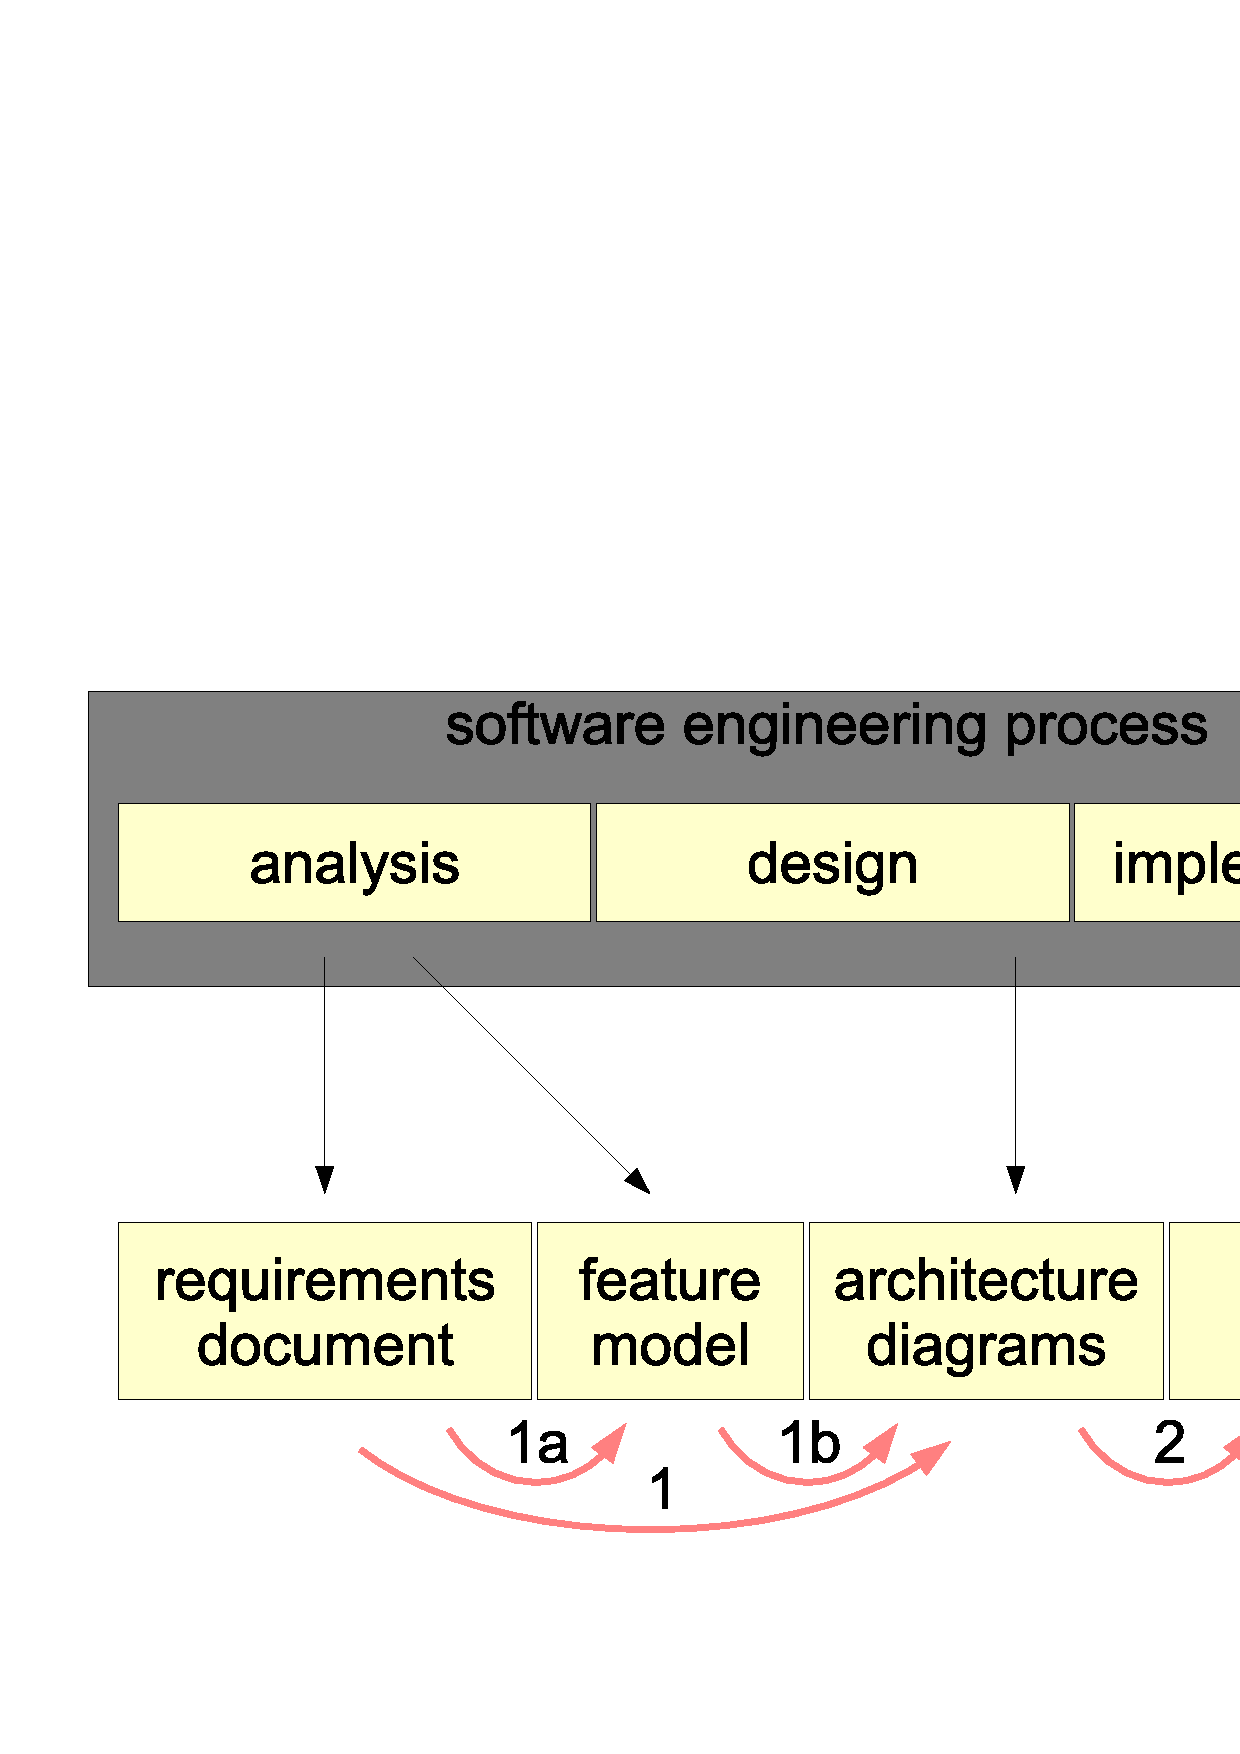
\includegraphics[scale=0.3,angle=-90]{graphics/gaps.pdf}
        \caption{Standard Software Engineering Process}
        \label{software_engineering_process_figure}
    \end{center}
\end{figure}

%
% $RCSfile$
%
% Copyright (c) 2005-2006. Christian Heller. All rights reserved.
%
% Permission is granted to copy, distribute and/or modify this document
% under the terms of the GNU Free Documentation License, Version 1.1 or
% any later version published by the Free Software Foundation; with no
% Invariant Sections, with no Front-Cover Texts and with no Back-Cover
% Texts. A copy of the license is included in the section entitled
% "GNU Free Documentation License".
%
% http://www.cybop.net
% - Cybernetics Oriented Programming -
%
% http://www.resmedicinae.org
% - Information in Medicine -
%
% Version: $Revision$ $Date$ $Author$
% Authors: Christian Heller <christian.heller@tuxtax.de>
%

\subsection{CYBOI}
\label{cyboi_heading}

The pure existence of proper knowledge does not suffice to create an improved
kind of software system, within a slimmer software development process. The
system needs to know how to \emph{handle} knowledge, at runtime. The criticism
is twofold, since traditionally:

\begin{enumerate}
    \item Operating systems don't have sufficient knowledge handling capabilities
    \item Applications contain too much low-level system control functionality
\end{enumerate}

This is changed when using CYBOI. As active interpreter encapsulating
system-level functionality, it handles knowledge provided in form of passive
CYBOL templates. In CYBOP systems, all compound knowledge models have the same
type structure (schema). Since they do not differ, they can be manipulated in
the same manner.

%
% $RCSfile$
%
% Copyright (c) 2005-2006. Christian Heller. All rights reserved.
%
% Permission is granted to copy, distribute and/or modify this document
% under the terms of the GNU Free Documentation License, Version 1.1 or
% any later version published by the Free Software Foundation; with no
% Invariant Sections, with no Front-Cover Texts and with no Back-Cover
% Texts. A copy of the license is included in the section entitled
% "GNU Free Documentation License".
%
% http://www.cybop.net
% - Cybernetics Oriented Programming -
%
% http://www.resmedicinae.org
% - Information in Medicine -
%
% Version: $Revision$ $Date$ $Author$
% Authors: Christian Heller <christian.heller@tuxtax.de>
%

\subsubsection{Overall Placement}
\label{overall_placement_heading}

Considering an overall computer system architecture, \emph{CYBOI} is situated
between the application knowledge existing in form of \emph{CYBOL} templates
and the \emph{Hardware} controlled by an \emph{Operating System} (OS) (figure
\ref{connection_figure}). CYBOI can thus also be called a
\emph{Knowledge-Hardware-Interface} (synonymous with \emph{Mind-Brain-Interface}).

\begin{figure}[ht]
    \begin{center}
        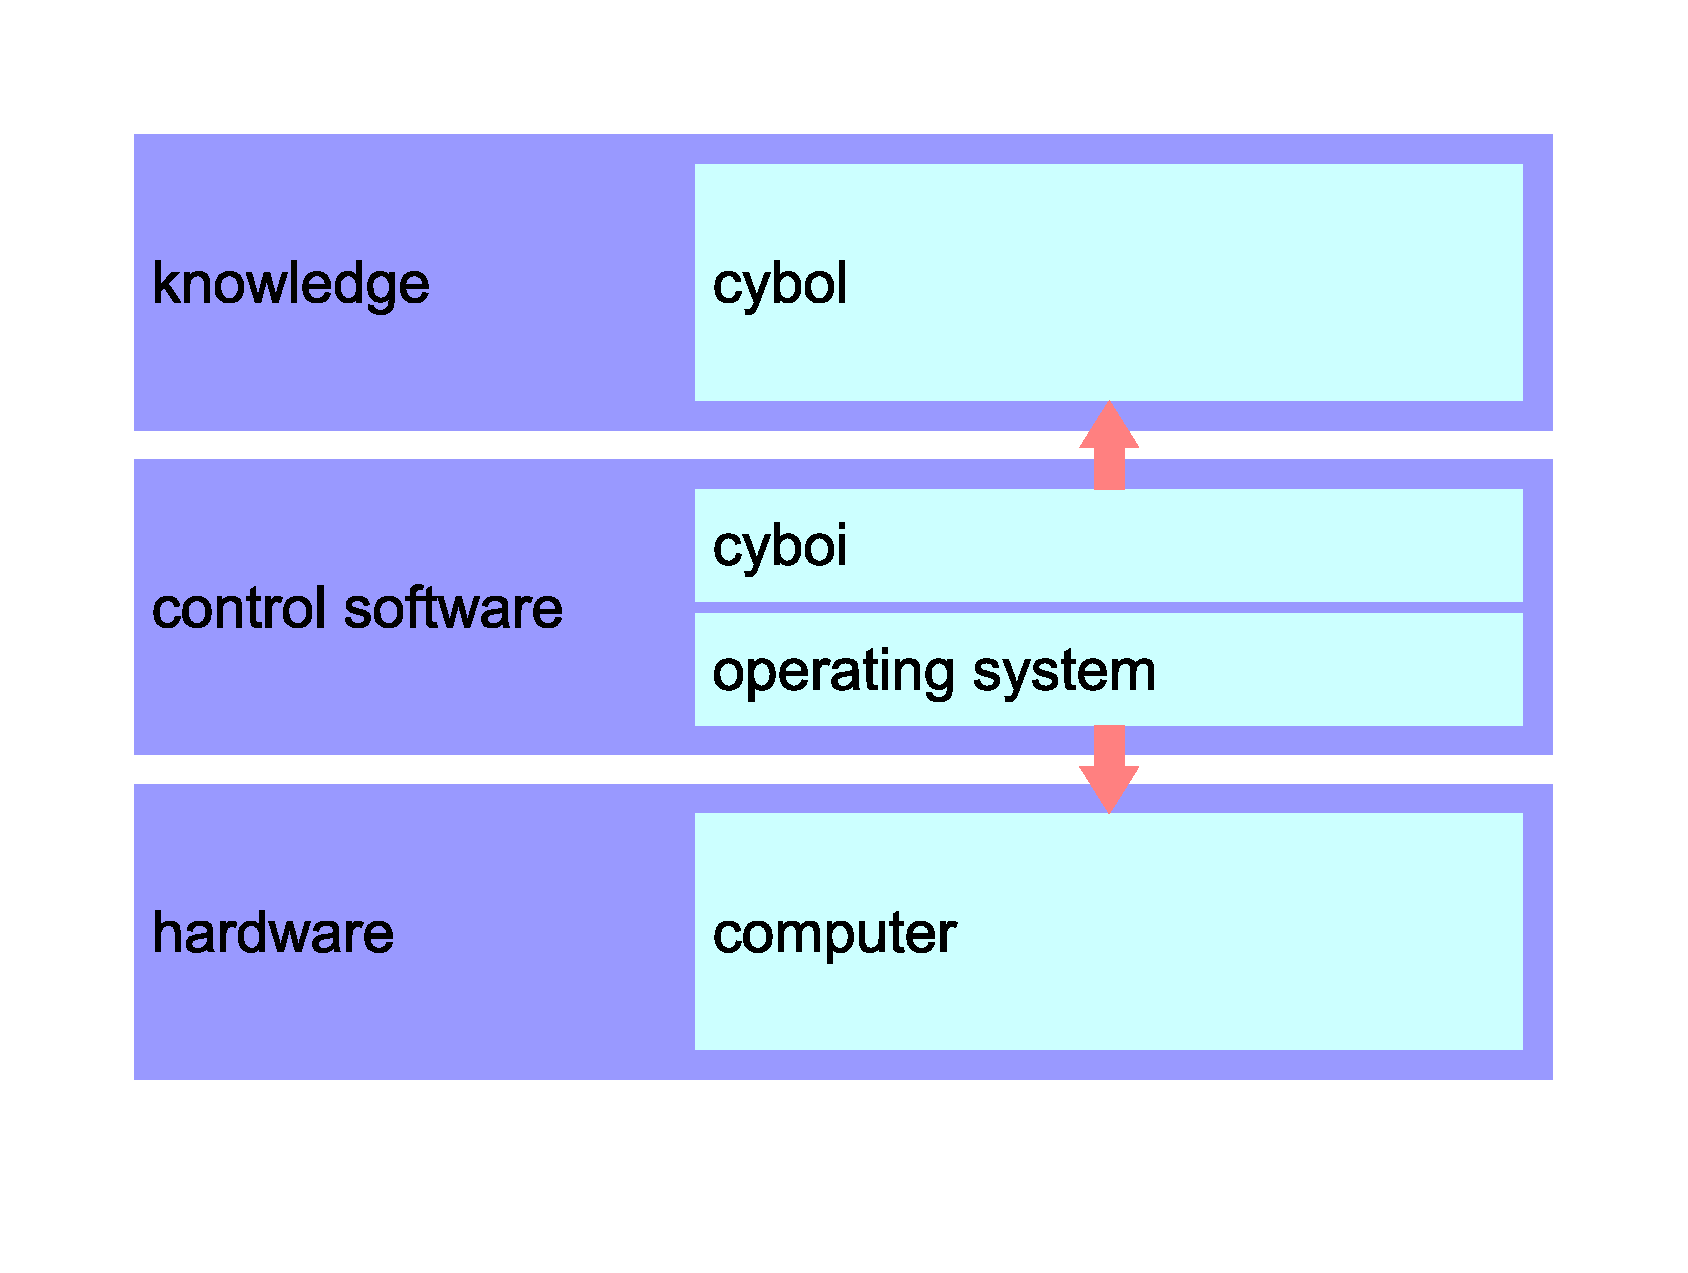
\includegraphics[scale=0.2]{vector/connection.eps}
        \caption{Knowledge -- Hardware Link}
        \label{connection_figure}
    \end{center}
\end{figure}

\begin{table}[ht]
    \begin{center}
        \begin{footnotesize}
        \begin{tabular}{| p{18mm} | p{18mm} | p{18mm} |}
            \hline
            \textbf{Criterion} & \textbf{Java World} & \textbf{CYBOP World}\\
            \hline
            Theory & OOP in Java & CYBOP\\
            \hline
            Language & Java & CYBOL\\
            \hline
            Interpreter & Java VM & CYBOI\\
            \hline
        \end{tabular}
        \end{footnotesize}
        \caption{Java-/ CYBOP World Analogies}
        \label{analogies_table}
    \end{center}
\end{table}

There are analogies to other systems run by language interpretation. Table
\ref{analogies_table} shows those between the \emph{Java-} and \emph{CYBOP}
world. Both are based on a programming theory, have a language and interpreter.
A theoretical model of a computer hardware- or -software system may be called
an \emph{Abstract Computer} or \emph{Abstract Machine} \cite{wikipedia}. If
being implemented as software simulation, or if containing an interpreter, it
is called a \emph{Virtual Machine} (VM). Kernighan and Pike write in their book
\emph{Practice of Programming} \cite{kernighan1999}:

\begin{quote}
� � Virtual machines are a wonderful, old idea, that latterly, through Java and
    the \emph{Java Virtual Machine} (JVM), came into fashion again. They are a
    simple possibility to gain portable and efficient program code, which can
    be written in a higher programming language.
\end{quote}

In that sense, CYBOI is certainly a VM. It provides low-level, platform-dependent
system functionality, close to the OS, together with a unified knowledge schema
(section \ref{knowledge_schema_heading}) which allows CYBOL applications to be
truly portable, well extensible and easier to program, because developers need
to concentrate on domain knowledge only. Since CYBOI interprets CYBOL sources
\emph{live} at system runtime, without the need for previous compilation (as in
Java), changes to CYBOL sources get into effect right away, without restarting
the system.

%
% $RCSfile$
%
% Copyright (c) 2005-2006. Christian Heller. All rights reserved.
%
% Permission is granted to copy, distribute and/or modify this document
% under the terms of the GNU Free Documentation License, Version 1.1 or
% any later version published by the Free Software Foundation; with no
% Invariant Sections, with no Front-Cover Texts and with no Back-Cover
% Texts. A copy of the license is included in the section entitled
% "GNU Free Documentation License".
%
% http://www.cybop.net
% - Cybernetics Oriented Programming -
%
% http://www.resmedicinae.org
% - Information in Medicine -
%
% Version: $Revision$ $Date$ $Author$
% Authors: Christian Heller <christian.heller@tuxtax.de>
%

\subsubsection{Architecture}
\label{architecture_heading}

To what concerns its inner architecture, there are two basic structures
underlying CYBOI:

\begin{enumerate}
    \item \emph{Knowledge Container:} An array-based structure usable for
        storing static knowledge in form of primitive- and compound models, and
        capable of representing a map, collection, list and tree
    \item \emph{Signal Checker:} A loop-based structure usable for dynamically
        reading signals from a queue, and capable of processing them after
        their priority, in a special handler
\end{enumerate}

\begin{figure}[ht]
    \begin{center}
        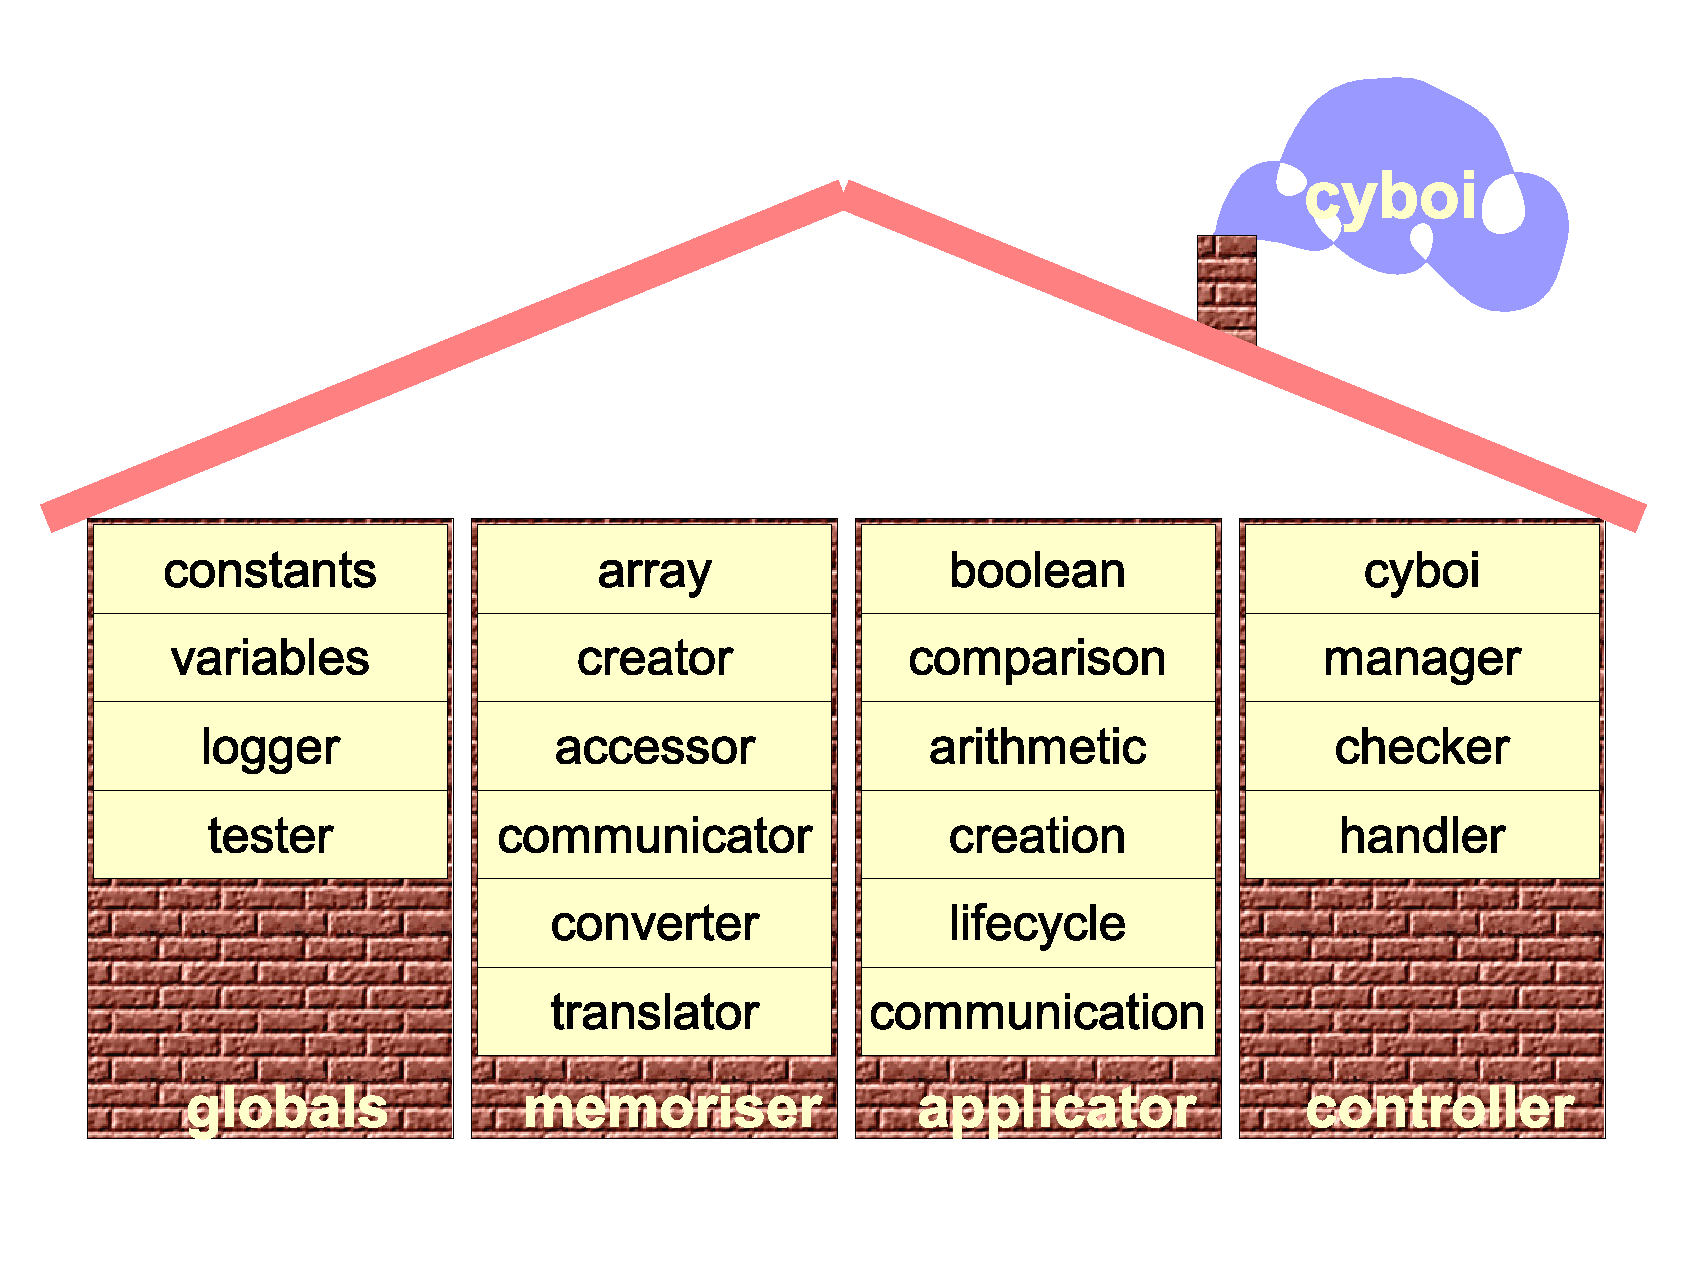
\includegraphics[scale=0.2]{vector/architecture.eps}
        \caption{CYBOI Architecture}
        \label{architecture_figure}
    \end{center}
\end{figure}

All modules, into which CYBOI is subdivided, are built around these two core
structures. Not unlike John von Neumann's model of a computing machine
\cite{selflinux}, which distinguishes \emph{Memory}, \emph{Control Unit},
\emph{Algorithmic Logic Unit} (ALU) and \emph{Input/ Output} (i/o), CYBOI's
modules are grouped into four architectural parts, as illustrated in figure
\ref{architecture_figure}. These have the following functionality:

\begin{itemize}
    \item \emph{Memoriser:} data creation, -destruction and -access (after
        Neumann, it contains not only data, but also the operations that are
        applied to them)
    \item \emph{Controller:} lifecycle management, signal handling, i/o filters
    \item \emph{Applicator:} operation application (comparison, logic,
        arithmetic and more)
    \item \emph{Globals:} basic constants and variables, as well as a logger
\end{itemize}

The i/o data handling is not separated out here (as opposed to von Neumann's
model); it is managed by the controller modules. The i/o data themselves,
representing states, are stored in memory.

%
% $RCSfile$
%
% Copyright (c) 2005-2006. Christian Heller. All rights reserved.
%
% Permission is granted to copy, distribute and/or modify this document
% under the terms of the GNU Free Documentation License, Version 1.1 or
% any later version published by the Free Software Foundation; with no
% Invariant Sections, with no Front-Cover Texts and with no Back-Cover
% Texts. A copy of the license is included in the section entitled
% "GNU Free Documentation License".
%
% http://www.cybop.net
% - Cybernetics Oriented Programming -
%
% http://www.resmedicinae.org
% - Information in Medicine -
%
% Version: $Revision$ $Date$ $Author$
% Authors: Christian Heller <christian.heller@tuxtax.de>
%

\subsubsection{Functionality}
\label{functionality_heading}

Figure \ref{cyboi_figure} shows three main parts of CYBOI. (The \emph{Globals}
package is neglectable for the following explanations, since it contains static
constants and variables that are \emph{omnipresent}.) The \emph{Controller}
manages system startup, shutdown and the handling of signals during its
runtime; the system uses just one central signal checking loop. The
\emph{Memoriser} provides memory structures (to store knowledge) and procedures
to access these. Logic knowledge is processed in the \emph{Applicator}.

\begin{figure}[ht]
    \begin{center}
        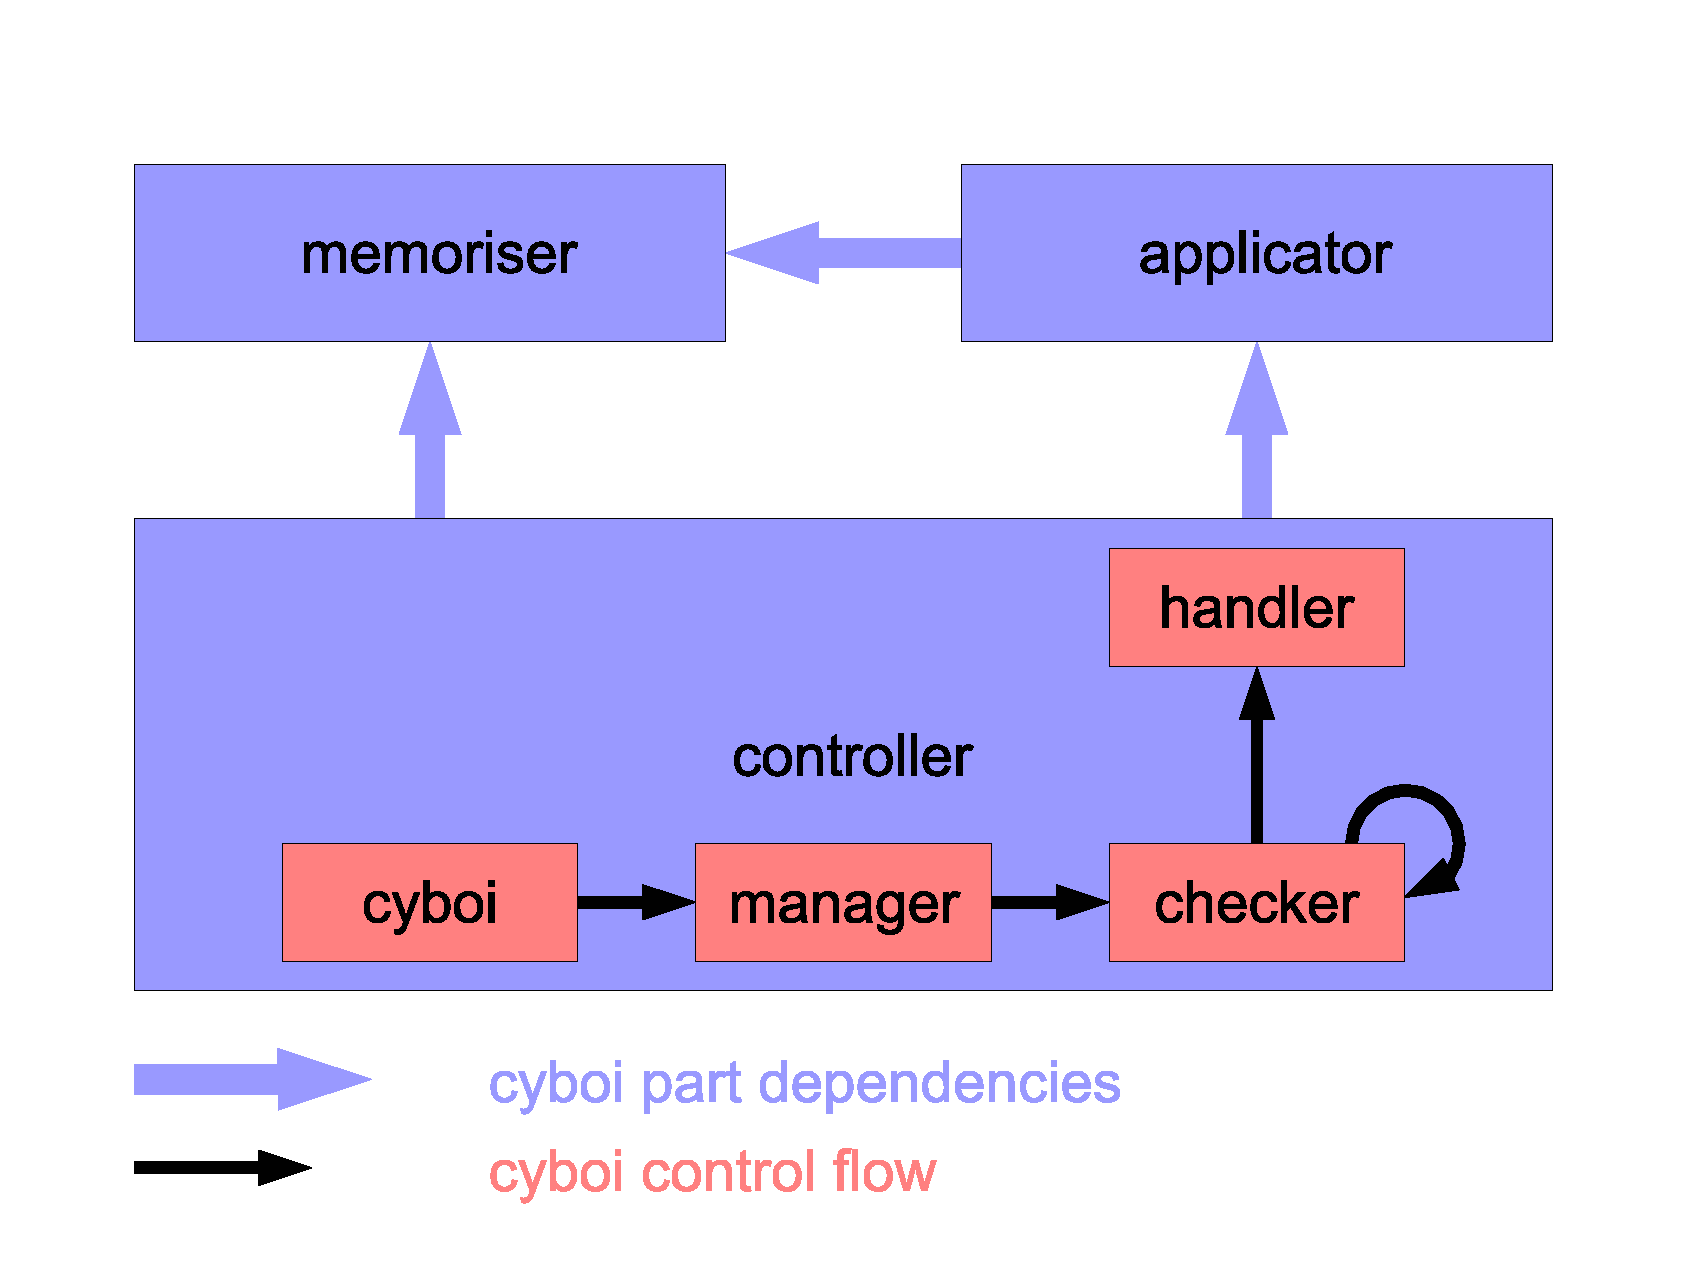
\includegraphics[scale=0.2]{vector/dependencies.eps}
        \caption{Dependencies and Control Flow}
        \label{cyboi_figure}
    \end{center}
\end{figure}


%
% $RCSfile: res_medicinae.tex,v $
%
% Copyright (C) 2002-2008. Christian Heller.
%
% Permission is granted to copy, distribute and/or modify this document
% under the terms of the GNU Free Documentation License, Version 1.1 or
% any later version published by the Free Software Foundation; with no
% Invariant Sections, with no Front-Cover Texts and with no Back-Cover
% Texts. A copy of the license is included in the section entitled
% "GNU Free Documentation License".
%
% http://www.cybop.net
% - Cybernetics Oriented Programming -
%
% http://www.resmedicinae.org
% - Information in Medicine -
%
% Version: $Revision: 1.1 $ $Date: 2008-08-19 20:41:08 $ $Author: christian $
% Authors: Christian Heller <christian.heller@tuxtax.de>
%

\chapter{Res Medicinae}
\label{res_medicinae_heading}
\index{Res Medicinae Application Prototype}

\begin{flushright}
    \textsl{
        No Road can ever be too long,\\
        side-by-side with a good Friend.
    }\\
    \textsc{Unknown Author}
\end{flushright}

The first two chapters (\ref{cybernetics_oriented_language_heading} and
\ref{cybernetics_oriented_interpreter_heading}) of part \ref{proof_heading} of
this work defined the CYBOL language and its corresponding interpreter CYBOI.
Since a theory is worth more if it can be proven in practice, this chapter will
describe an effort trying to apply both to create an application system named
\emph{Res Medicinae} \cite{resmedicinae} (Latin for \emph{Matter of Medicine}).

%
% $RCSfile: project.tex,v $
%
% Copyright (C) 2002-2008. Christian Heller.
%
% Permission is granted to copy, distribute and/or modify this document
% under the terms of the GNU Free Documentation License, Version 1.1 or
% any later version published by the Free Software Foundation; with no
% Invariant Sections, with no Front-Cover Texts and with no Back-Cover
% Texts. A copy of the license is included in the section entitled
% "GNU Free Documentation License".
%
% http://www.cybop.net
% - Cybernetics Oriented Programming -
%
% http://www.resmedicinae.org
% - Information in Medicine -
%
% Version: $Revision: 1.1 $ $Date: 2008-08-19 20:41:08 $ $Author: christian $
% Authors: Christian Heller <christian.heller@tuxtax.de>
%

\section{Project}
\label{project_heading}
\index{Res Medicinae Project}
\index{Hospital Information System}
\index{HIS}
\index{Practice Management System}
\index{PMS}
\index{Electronic Health Record}
\index{EHR}

The -- somewhat idealistic -- aim was initially to create the prototype of a
\emph{Hospital Information System} (HIS). Due to the clearly too high-set aims,
this was later revised so that the focus of the prototype became a standard
\emph{Practice Management System} (PMS) with an \emph{Electronic Health Record}
(EHR) as its core. Several technology changes during the progress of this work
and the lack in time required to also revise this aim, so that now the final
prototype consists of just the (rudimentary) address management module of the
planned EHR application. It is written in CYBOL and executable by CYBOI.

The following sections describe the project background of \emph{Res Medicinae}.

\input{free_and_open_source_software}
\input{portals_and_services}
\input{tools}
\input{contributors}

%
% $RCSfile: analysis.tex,v $
%
% Copyright (C) 2002-2008. Christian Heller.
%
% Permission is granted to copy, distribute and/or modify this document
% under the terms of the GNU Free Documentation License, Version 1.1 or
% any later version published by the Free Software Foundation; with no
% Invariant Sections, with no Front-Cover Texts and with no Back-Cover
% Texts. A copy of the license is included in the section entitled
% "GNU Free Documentation License".
%
% http://www.cybop.net
% - Cybernetics Oriented Programming -
%
% http://www.resmedicinae.org
% - Information in Medicine -
%
% Version: $Revision: 1.1 $ $Date: 2008-08-19 20:41:05 $ $Author: christian $
% Authors: Christian Heller <christian.heller@tuxtax.de>
%

\section{Analysis}
\label{analysis_heading}
\index{Res Medicinae Requirements Analysis}
\index{Software Engineering Process}
\index{SEP}
\index{Electronic Health Record}
\index{EHR}

Abiding by the standard \emph{Software Engineering Process} (SEP) (chapter
\ref{software_engineering_process_heading}), a \emph{Requirements Analysis}
stood as first activity for the development of \emph{Res Medicinae}. The
following sections will give a brief overview of some requirements and current
modelling trends, concerning the \emph{Electronic Health Record} (EHR). They do
\emph{not} try to replace more comprehensive works written on the subject.

\input{requirements_document}
\input{ehr_and_co}
\input{episode_based}
\input{evidence_based}
\input{continuity_of_care}
\input{core_model}

\newpage
%
% $RCSfile: standards.tex,v $
%
% Copyright (C) 2002-2008. Christian Heller.
%
% Permission is granted to copy, distribute and/or modify this document
% under the terms of the GNU Free Documentation License, Version 1.1 or
% any later version published by the Free Software Foundation; with no
% Invariant Sections, with no Front-Cover Texts and with no Back-Cover
% Texts. A copy of the license is included in the section entitled
% "GNU Free Documentation License".
%
% http://www.cybop.net
% - Cybernetics Oriented Programming -
%
% http://www.resmedicinae.org
% - Information in Medicine -
%
% Version: $Revision: 1.1 $ $Date: 2008-08-19 20:41:09 $ $Author: christian $
% Authors: Christian Heller <christian.heller@tuxtax.de>
%

\section{Standards}
\label{standards_heading}
\index{Medical Informatics Standards}

In a further thought, current standards of medical informatics had to be
considered for the development of \emph{Res Medicinae} application modules.
There exists a whole plethora of (partly \emph{de facto}) standards -- far too
many to discuss here. The following sections will give a brief overview of only
a few standards which are potentially important for EHR development.

\input{overview}
\input{record_modelling}
\input{messaging_and_communication}
\input{terminology_systems}
\input{further_standards}
\input{standards_development}
\input{implication}

%
% $RCSfile: realisation.tex,v $
%
% Copyright (C) 2002-2008. Christian Heller.
%
% Permission is granted to copy, distribute and/or modify this document
% under the terms of the GNU Free Documentation License, Version 1.1 or
% any later version published by the Free Software Foundation; with no
% Invariant Sections, with no Front-Cover Texts and with no Back-Cover
% Texts. A copy of the license is included in the section entitled
% "GNU Free Documentation License".
%
% http://www.cybop.net
% - Cybernetics Oriented Programming -
%
% http://www.resmedicinae.org
% - Information in Medicine -
%
% Version: $Revision: 1.1 $ $Date: 2008-08-19 20:41:08 $ $Author: christian $
% Authors: Christian Heller <christian.heller@tuxtax.de>
%

\section{Realisation}
\label{realisation_heading}
\index{Res Medicinae Steps of Realisation}

Having analysed the domain of healthcare and having investigated corresponding
standards, actual design solutions that have been tried out in the course of
this work, by implementing them in software source code, can be described in
the following sections.

\input{student_works}
\input{first_trial}
\input{knowledge_separation}
\input{reimplementation}
\input{module_modelling}



    %
% $RCSfile: summary.tex,v $
%
% Copyright (c) 2001-2004. Christian Heller. All rights reserved.
%
% Permission is granted to copy, distribute and/or modify this document
% under the terms of the GNU Free Documentation License, Version 1.1
% or any later version published by the Free Software Foundation;
% with no Invariant Sections, with no Front-Cover Texts and with no Back-Cover
% Texts. A copy of the license is included in the section entitled
% "GNU Free Documentation License".
%
% http://www.cybop.net
% - Cybernetics Oriented Programming -
%
% http://www.resmedicinae.org
% - Information in Medicine -
%
% @author Christian Heller <christian.heller@tuxtax.de>
% @author Jens Bohl <info@jens-bohl.de>
%

\section{Summary}
\label{summary_heading}

Software design patterns are essential elements of frameworks. They can be
combined to comprise their advantages and to realize hierarchical structures.
These structures can be created and destroyed in the lifecycle of components.
In that lifecycle, object relations become more transparent and are easier to
control and to maintain.\\
Ontologies can help to model particular domains and to layer software. Every level
of these ontologies has a particular supertype, whereby these types depend on each
other by inheritance. This concept supports the modelling and logical separation
of software into hierarchical architectures. The granularity of the ontology
(number of ontological levels) can be adapted to particular requests.\\
By applying the new concepts introduced in this document, the quality of software
can be greatly increased. The time for building systems can be reduced to a minimum.
The clear architecture avoids common confusion as the systems grow.


    \bibliography{references}
\end{document}
